\chapter{The LHC and the ATLAS Detector}
\label{chap_detector}

%Hi Pete,
%
%   A scan of my marked-up version is attached. I have some general comments as 
%well, which I will just write here.
%
%   To start, let me remark that there are a number of places where you describe things 
%in terms of design parameters (luminosity, EF output rate in the trigger discussion, 
%number of bunches in the LHC etc) but don't also make reference to what the current 
%values are (or what they were for the 2010 data taking that you are discussing).   
%

%   Next, while I think for completeness you do need to mention the overall structure
%of the detector, unless I'm forgetting some aspect of your jet analysis, there seems to
%be no real motivation for detailed discussions of the ID or MS.  Your discussion of 
%each of these are indeed currently brief, but have details that I think are unnecessary 
%in the context of your thesis. The things you need to focus on are the calorimeters and 
%the trigger system. While you do spend more time on each of these,  they both need 
%work. (I don't recall if you have any systematic studies using track jets. If that were the
%case then perhaps you would need more on the ID).
%
%   For the calorimeter section, you don't address fairly basic issues like why liquid argon
%is chosen as the active material for most of the calorimeter (and why you can get away
%with scintillating tiles in the barrel hadronic calorimeter). I may be wrong, but it seems
%as if the details that are provided in the section are somewhat random. What you need 
%to focus on are those details of  the calorimeter that are most important to the jet analysis.
%And of course you do need a special focus on the FCal, since it is the most relevant 
%detector for both of the topics in your thesis. But as another example of where relevant
%detail is lacking, on page 12 you give a reason for why the FCal LAr gaps are so small,
%but don't say why the positive ion buildup is a problem.  You will need to decide what 
%part of the FCal description goes here and what can been discussed in the testbeam 
%chapters.  But I think you need more discussion of the FCal than you have here.
%
%   For the trigger discussion, I again think this needs to focus on the issues most relevant
%to your analysis. Maybe this is already the case, but I would like to see a somewhat more
%detailed discussion than you have in the 2+ pages you currently have on this topic.
%
%   That's all for now.
%
%        - Peter


%todo:
% - add "many references"
% - MBTS
%
%things to add
%precision measurements up to 2.5 in eta, but coverage up to ~5
%hardware/software of the trigger. capable of >200Hz now


\section{The Large Hadron Collider}

%%%%%%%%%%%%%%%%%%%%%%%%%%%%%%%%%%%%%%%
%%%%%%%%%%%%%%%%%%%%%%%%%%%%%%%%%%%%%%%
%comments from PK:
%quoted design parameters, quote values of luminosity, etc for 2010
%check trigger rate, 200 Hz at EF, PK says 400 HZ+
%
%
%more stuff in calorimeter section. 
%motivate design choices, why the accordion shape in the barrel/emec
%why scintillator in the Tile?
%why copper/LAr in the HEC?
%why is positive ion build up bad ? (interferes with the field in the electrode/messes up drift?)
%
%more detail in trigger section, specifically related to jets.
%L1 algorithms /L2 algorithms
%
%L1_FJ10 looks for 10 GeV forward jets, seeds l2_fj25, 25 GeV forward jets., etc.


%%%%%%%%%%%%%%%%%%%%%%%%%%%%%%%%%%%%%%%%%
%%%%%%%%%%%%%%%%%%%%%%%%%%%%%%%%%%%%%%%%%

%The Large Hadron \cmt{change this} Collider (LHC)
%LHC, big accelerator
%
%feeds beam to ATLAS, CMS, LHCb, ALICE
%
%
%27km circumference
%
%between 45m and 170m underground
%
%crosses swiss-french border four times
%
%
%designed for 7 TeV/beam, protons
%
%
%2808 bunches, 10^11 protons/bunch
%
%design luminosity
%
%luminosity at the end of 2011
%
%
%linac2 - 50 MeV
%
%PSB (proton Synchrotron booster) 1.4 GeV
%
%PS (Proton synchrotron) 25 GeV
%
%SPS Super Proton Synchrotron 450 GeV
%
%LHC  design 7 TeV/beam, currently 3.5 TeV/beam
%
%at design luminosity of 10^34 cm^-2 s^-1, expect about 19 interactions per bunch crossing
%
%bunches cross every 25ns, interactions at a rate of 40 MHz
%
%currently running at a luminosity of XX cm ^-2 s^-1

%%%%%%%%%%%%%%%%%%%%%%%%%%%%%%%%%%%%%%%%%
%to do
%
%tidy LHC bit
%
%tidy coordinates bit
%
%pics:
%
%TiLE
%HEC







%%%%%%%%%%%%%%%%%%%%%%%%%%%%%%%%%%%%%%%%%%



%emmitance/acceptance?
%superconducting rf cavities
%pile up/ scatters per bunch crossing
%
%feeds a bunch of experiments, LHCb, ALICE, CMS, ATLAS
%
%fed by SPS, which is fed by PS, which is fed by ...
%luminosity still ramping up to design 
%presently at 3.5 TeV/beam with luminosity of ZZ

%when did it start?
%when is 7 TeV/beam expected?


The Large Hardon Collider (LHC)\cite{LHC_paper} is a particle collider situated near Geneva, Switzerland. It is  27km in circumference and is located between 45m and 170m underground, crossing the Swiss-French border four times. It is designed to accelerate two beams of protons to energies of 7 TeV, and to collide these beams at four points along its circumference with  instantaneous luminosities of up to $10^{34} \mathrm{cm}^{-2} \mathrm{s}^{-1}$. At present protons in the LHC are being accelerated to 4 TeV per beam, which is a slightly more than half of the design energy, while the maximum instantaneous luminosity being achieved is currently around $\sim 8\times 10^{33} \mathrm{cm}^{-2} \mathrm{s}^{-1}$ . The LHC is also capable of accelerating heavy ions to high energy. The ALICE experiment is focused on analysing these heavy ion collisions, while both \atlas and \cms also have heavy ion programs. % \blue{However, at the end of 2011 the LH an instantaneous luminosity }

\begin{figure}[tb]
\begin{center}
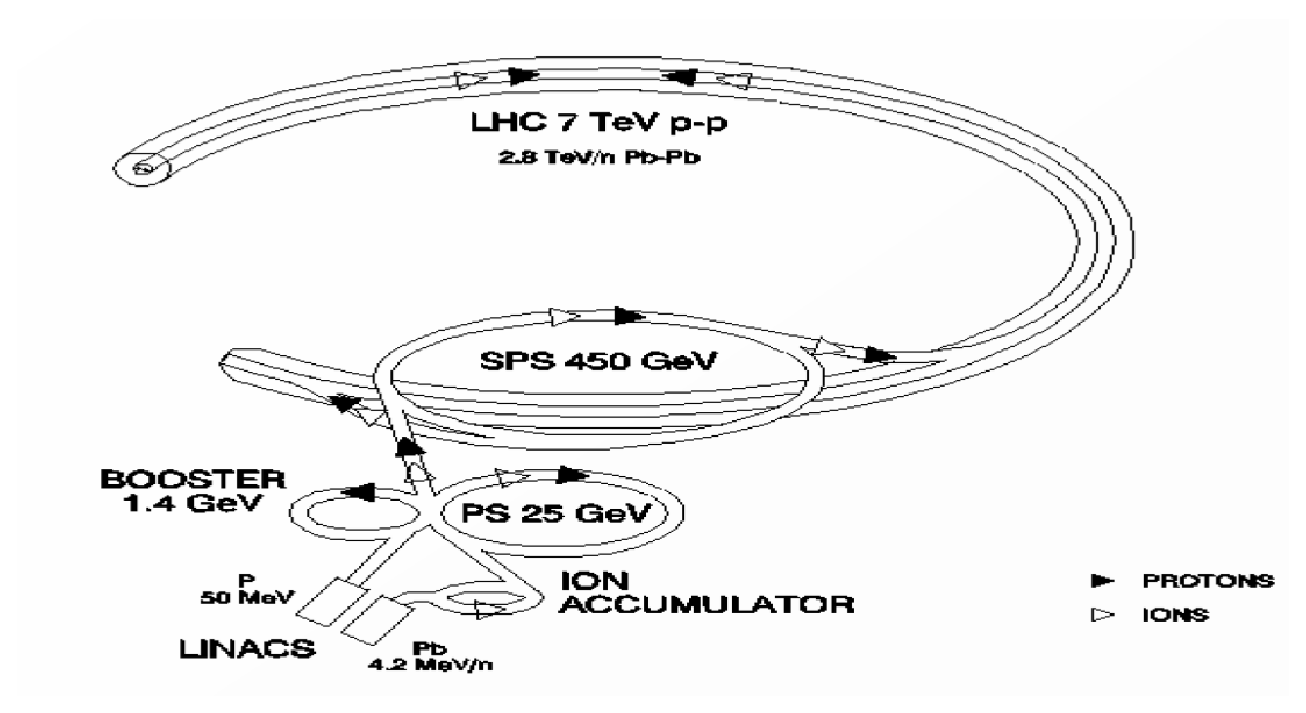
\includegraphics[width=0.6\linewidth,angle=0]{Detector/LHC_injection}
\end{center}
%\centerline{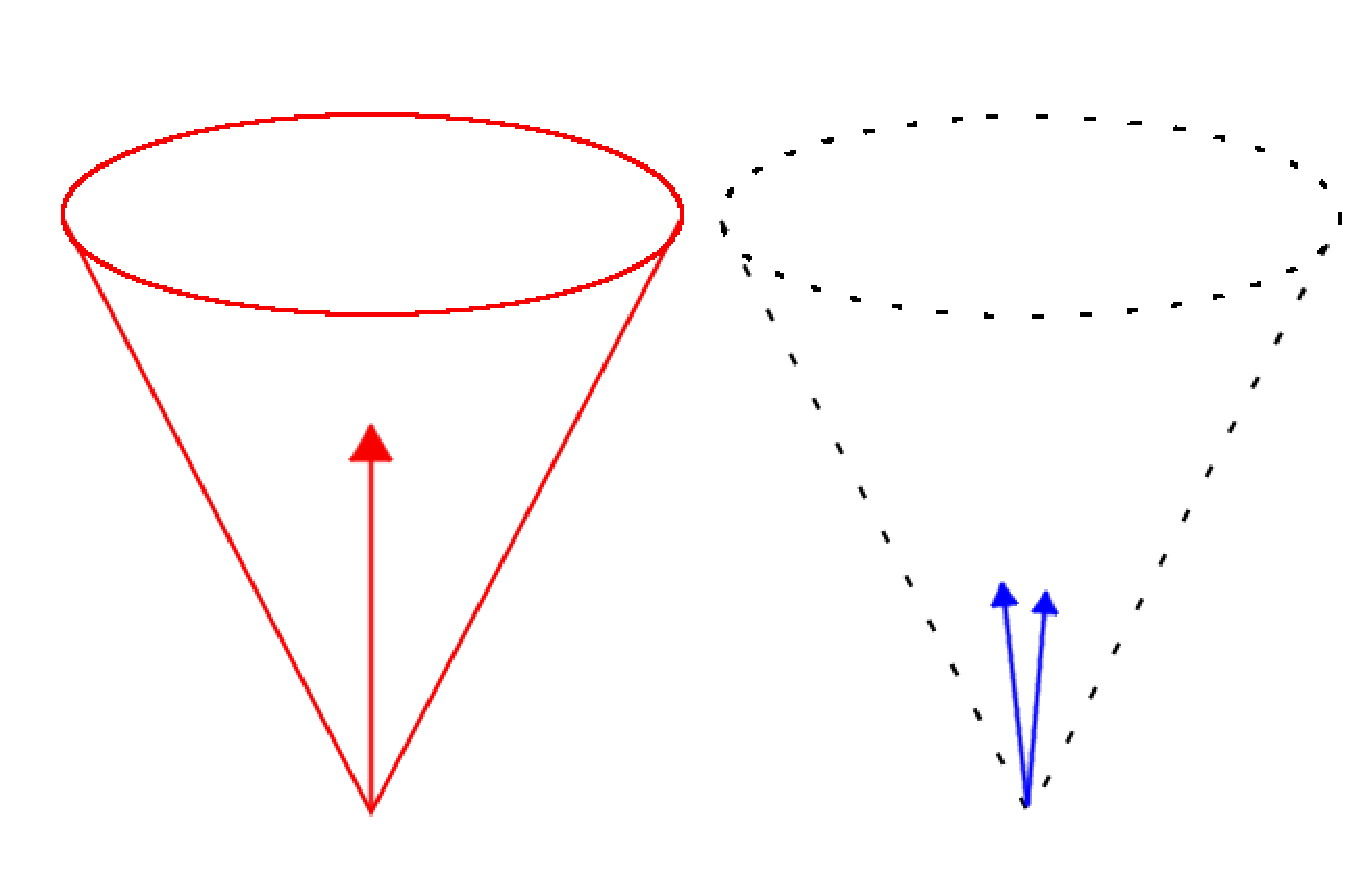
\epsfig{file=./figs/collinear.eps  , width=0.95\textwidth}}
\caption{Injection chain for protons and ions feeding the LHC. }
\label{LHC_inject}
\end{figure}

The injection chain for beam particles is shown in Figure~\ref{LHC_inject}. Hydrogen gas is used as a source of protons. Gas molecules are ionised in a duoplasmotron\cite{LHC_proton_source}, which emits protons at an energy of 90 keV. The protons are then accelerated to 750 KeV in a Radio Frequency Quadrupole (RFQ) before being accelerated to 50 MeV in a linear accelerator (LINAC2). A series of synchrotrons (the Proton Synchrotron Booster (PSB), Proton Synchrotron (PS), and Super Proton Synchrotron (SPS))  are then used to accelerate protons to energies of 1.4 GeV, 25 GeV and 450 GeV, respectively. After acceleration by the SPS, beams are injected into the LHC. Superconducting Radio-Frequency (RF) cavities are then used to accelerate the protons to their final energy.  Each LHC beam is designed to hold up to 2808 bunches\footnote{Currently only half of these bunches are being filled, such that bunch crossings are seperated by 50 ns.}, each containing $\sim 10^{11}$ protons, which are separated in time by 25 ns. 

%integrated/instantaneous relative to design
%
%expected to be operating at design parameters by 
%
%The proton beams are then injected into the LHC, 


\section{The ATLAS Detector}
The \atlas detector\cite{detector_paper} (shown in Figure~\ref{fig_ATLAS}) is a multi-purpose detector used to analyse collisions at the LHC. It is one of two multi-purpose detectors, the other being the Compact Muon Solenoid (CMS)\cite{CMSdetector}. \atlas consists of sophisticated particle tracking systems, a system of calorimeters, and a Muon Spectrometer, each of which will be discussed below. The Inner Detector (ID) and Muon Spectrometer (MS) will be discussed only briefly, as they play little role in the analyses discussed in this thesis. This chapter will focus on the calorimeters of \atlas, as these are used to reconstruct jets. Particular attention is paid to the forward calorimeters, as one of these was the subject of the beam test discussed in Chapter~\ref{chapTB}, and also because the forward calorimeters are responsible for the large kinematic coverage achieved in the inclusive jet and dijet cross-section measurements that are described in Chapter~\ref{INCJETCHAPTER}.
\begin{figure}[tb]
\begin{center}
\includegraphics[width=0.8\linewidth,angle=0]{Detector/ATLAS_overview}
\end{center}
%\centerline{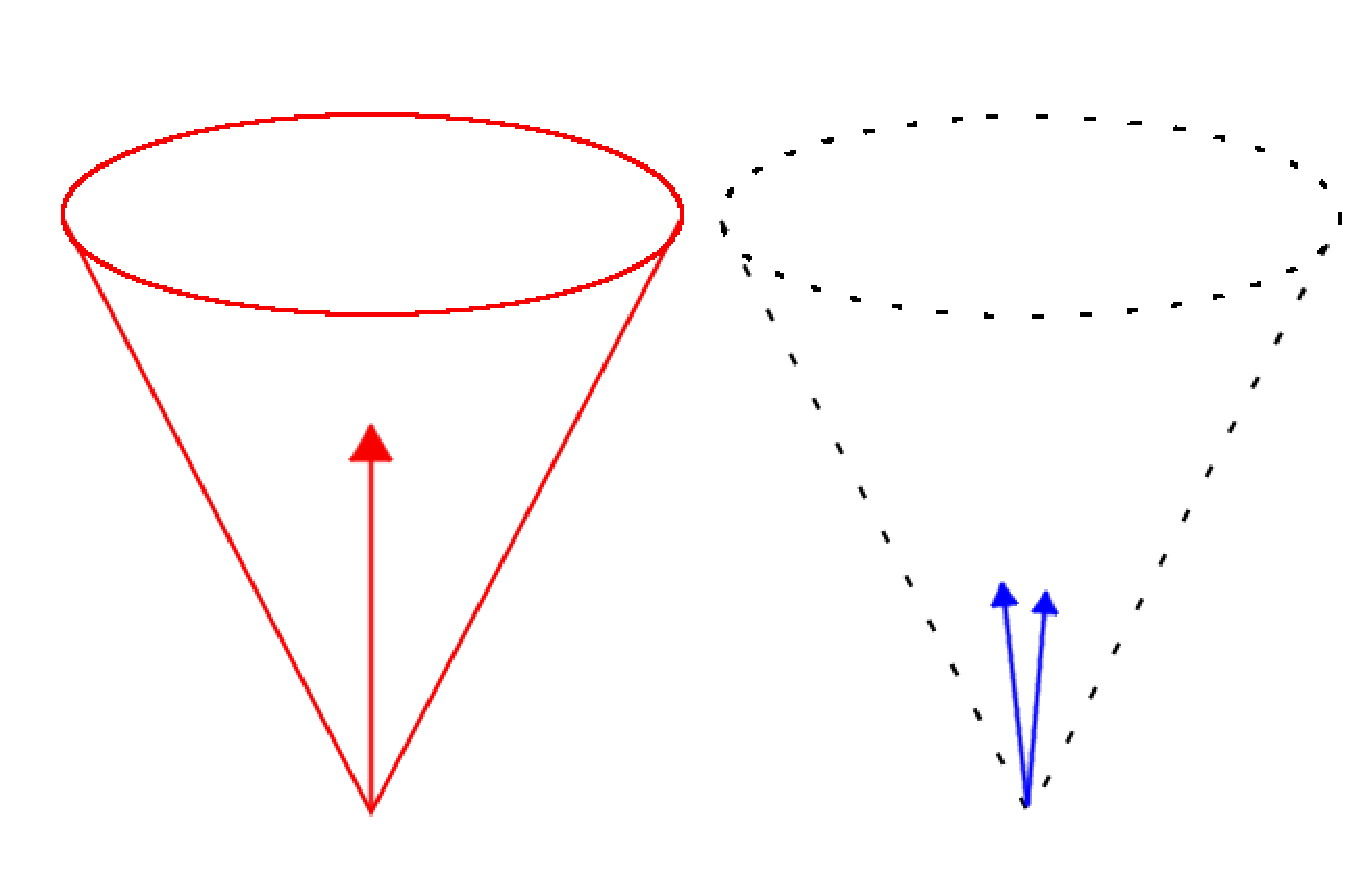
\epsfig{file=./figs/collinear.eps  , width=0.95\textwidth}}
\caption{Diagram of the ATLAS detector.}
\label{fig_ATLAS}
\end{figure}

\subsection{Coordinates}

\atlas uses a right-handed Cartesian coordinate system. The nominal interaction point at the centre of \atlas is defined to be the origin of this coordinate system, with the beams running along the $z$ axis. The positive $x$ axis points towards the centre of the LHC ring, while the positive $y$ axis is perpendicular to the other two, and points upwards. Parts of the detector are labelled according to which side of the interaction point they are located on. The ``A-side'' refers to objects located at positive values of $z$, while objects located at negative $z$ are said to be on the ``C-side''\cmt{which is especially nice during the summer}. \atlas is divided into a barrel and two end-cap sections. Each of these sections contains a cryostat, as (most of) the \atlas calorimetry is based on liquid argon technology.


The polar angle $\theta$ defines the angle from the beam axis, while the azimuthal angle $
\phi$ defines the angle around the beam axis. The direction $\theta = 0$ points along the positive $z$ axis, while $\phi = 0$ corresponds to the positive $x$ axis. The pseudorapidity, $\eta$, is defined using the polar angle $\theta$, such that 
\begin{equation}
\eta = - \log \left( \tan \left( \frac{\theta}{2} \right) \right).
\label{eqn_pseudorapidity}
\end{equation}
Pseudorapidity is an approximation to rapidity, $y$. The rapidity of an object with energy $E$ is given by
\begin{equation}
y = \frac{1}{2} \log \left(\frac{E+p_z}{E - p_z}\right),
\label{eqn_rapidity}
\end{equation}
where $p_z$ is the $z$ component of the objects momentum. The rapidity may be used to define a boost along the $z$ axis, such that in the boosted frame of reference the object's momentum will be perpendicular to the beam direction. In the limit where the mass of the object is negligible, pseudorapidity and rapidity are equivalent. Detector regions are typically described in terms of $\eta$, due to the one-to-one correspondence with $\theta$. Rapidity is often used when discussing kinematics, as differences in rapidity are invariant with respect to boosts in the direction of the beam.




 

%blah blah \atlas is blah blah



%\section{Coordinates}
%
%nominal interaction point defined as origin
%
%beam runs along z axis
%
%A side is positive z, C side negative
%
%positive x points towards centre of LHC ring
%
%positive y points up
%
%azimuthal angle, phi = 0 means in the x-z plane
%
%pseudorapidity defined as
%
%rapidity is ..., in the case of massive objects


%maybe?
\subsection{Inner Detector}
The Inner Detector (ID) is used to reconstruct the trajectories (tracks) of charged particles produced during proton-proton collisions. It is comprised of three systems: the pixel detector, the SemiConductor Tracker (SCT), and the Transition Radiation Tracker (TRT). These three components are contained within a cylindrical region of length 3.5m and radius 1.15m centred on the \atlas interaction point. The \atlas solenoid is a superconducting magnet located just outside of the ID, in the barrel cryostat, and generates a 2T magnetic field oriented along the $z$ axis in the region occupied by the ID. The applied field gives rise to curvature in the trajectories of charged particles, such that measurements of particle trajectories can be used to determine the transverse momentum (\pt) of those particles. The ID is also used for vertex reconstruction at \atlas. The primary vertex is associated with the location of the hard inelastic collision, while other soft collisions may produce additional secondary vertices. The accuracy with which a given vertex position may be reconstructed is dependent on the number of tracks associated with the vertex and the \pt~of those tracks. In cases where there are at least 70 tracks emerging from the primary vertex and the quadratic sum of track \pt~ values\cmt{when added in quadrature} exceeds 8 GeV, the primary vertex can be determined with an accuracy of $\sim$30 $\mu$m in the transverse plane and $\sim$50 $\mu$m in the longitudinal direction\cite{vertex_ref}.

%primary vertex -> hard inelastic collision location
%accuracy dependant on tracks.
%resolution

%which can then be used to obtain measurements the transverse momentum (\pt) of the track.

The inner detector consists of a barrel section (shown in Figure ~\ref{fig_ID_barrel}) and two end-cap sections (Figure \ref{fig_ID_EC}). 
\begin{figure}[p]
\begin{center}
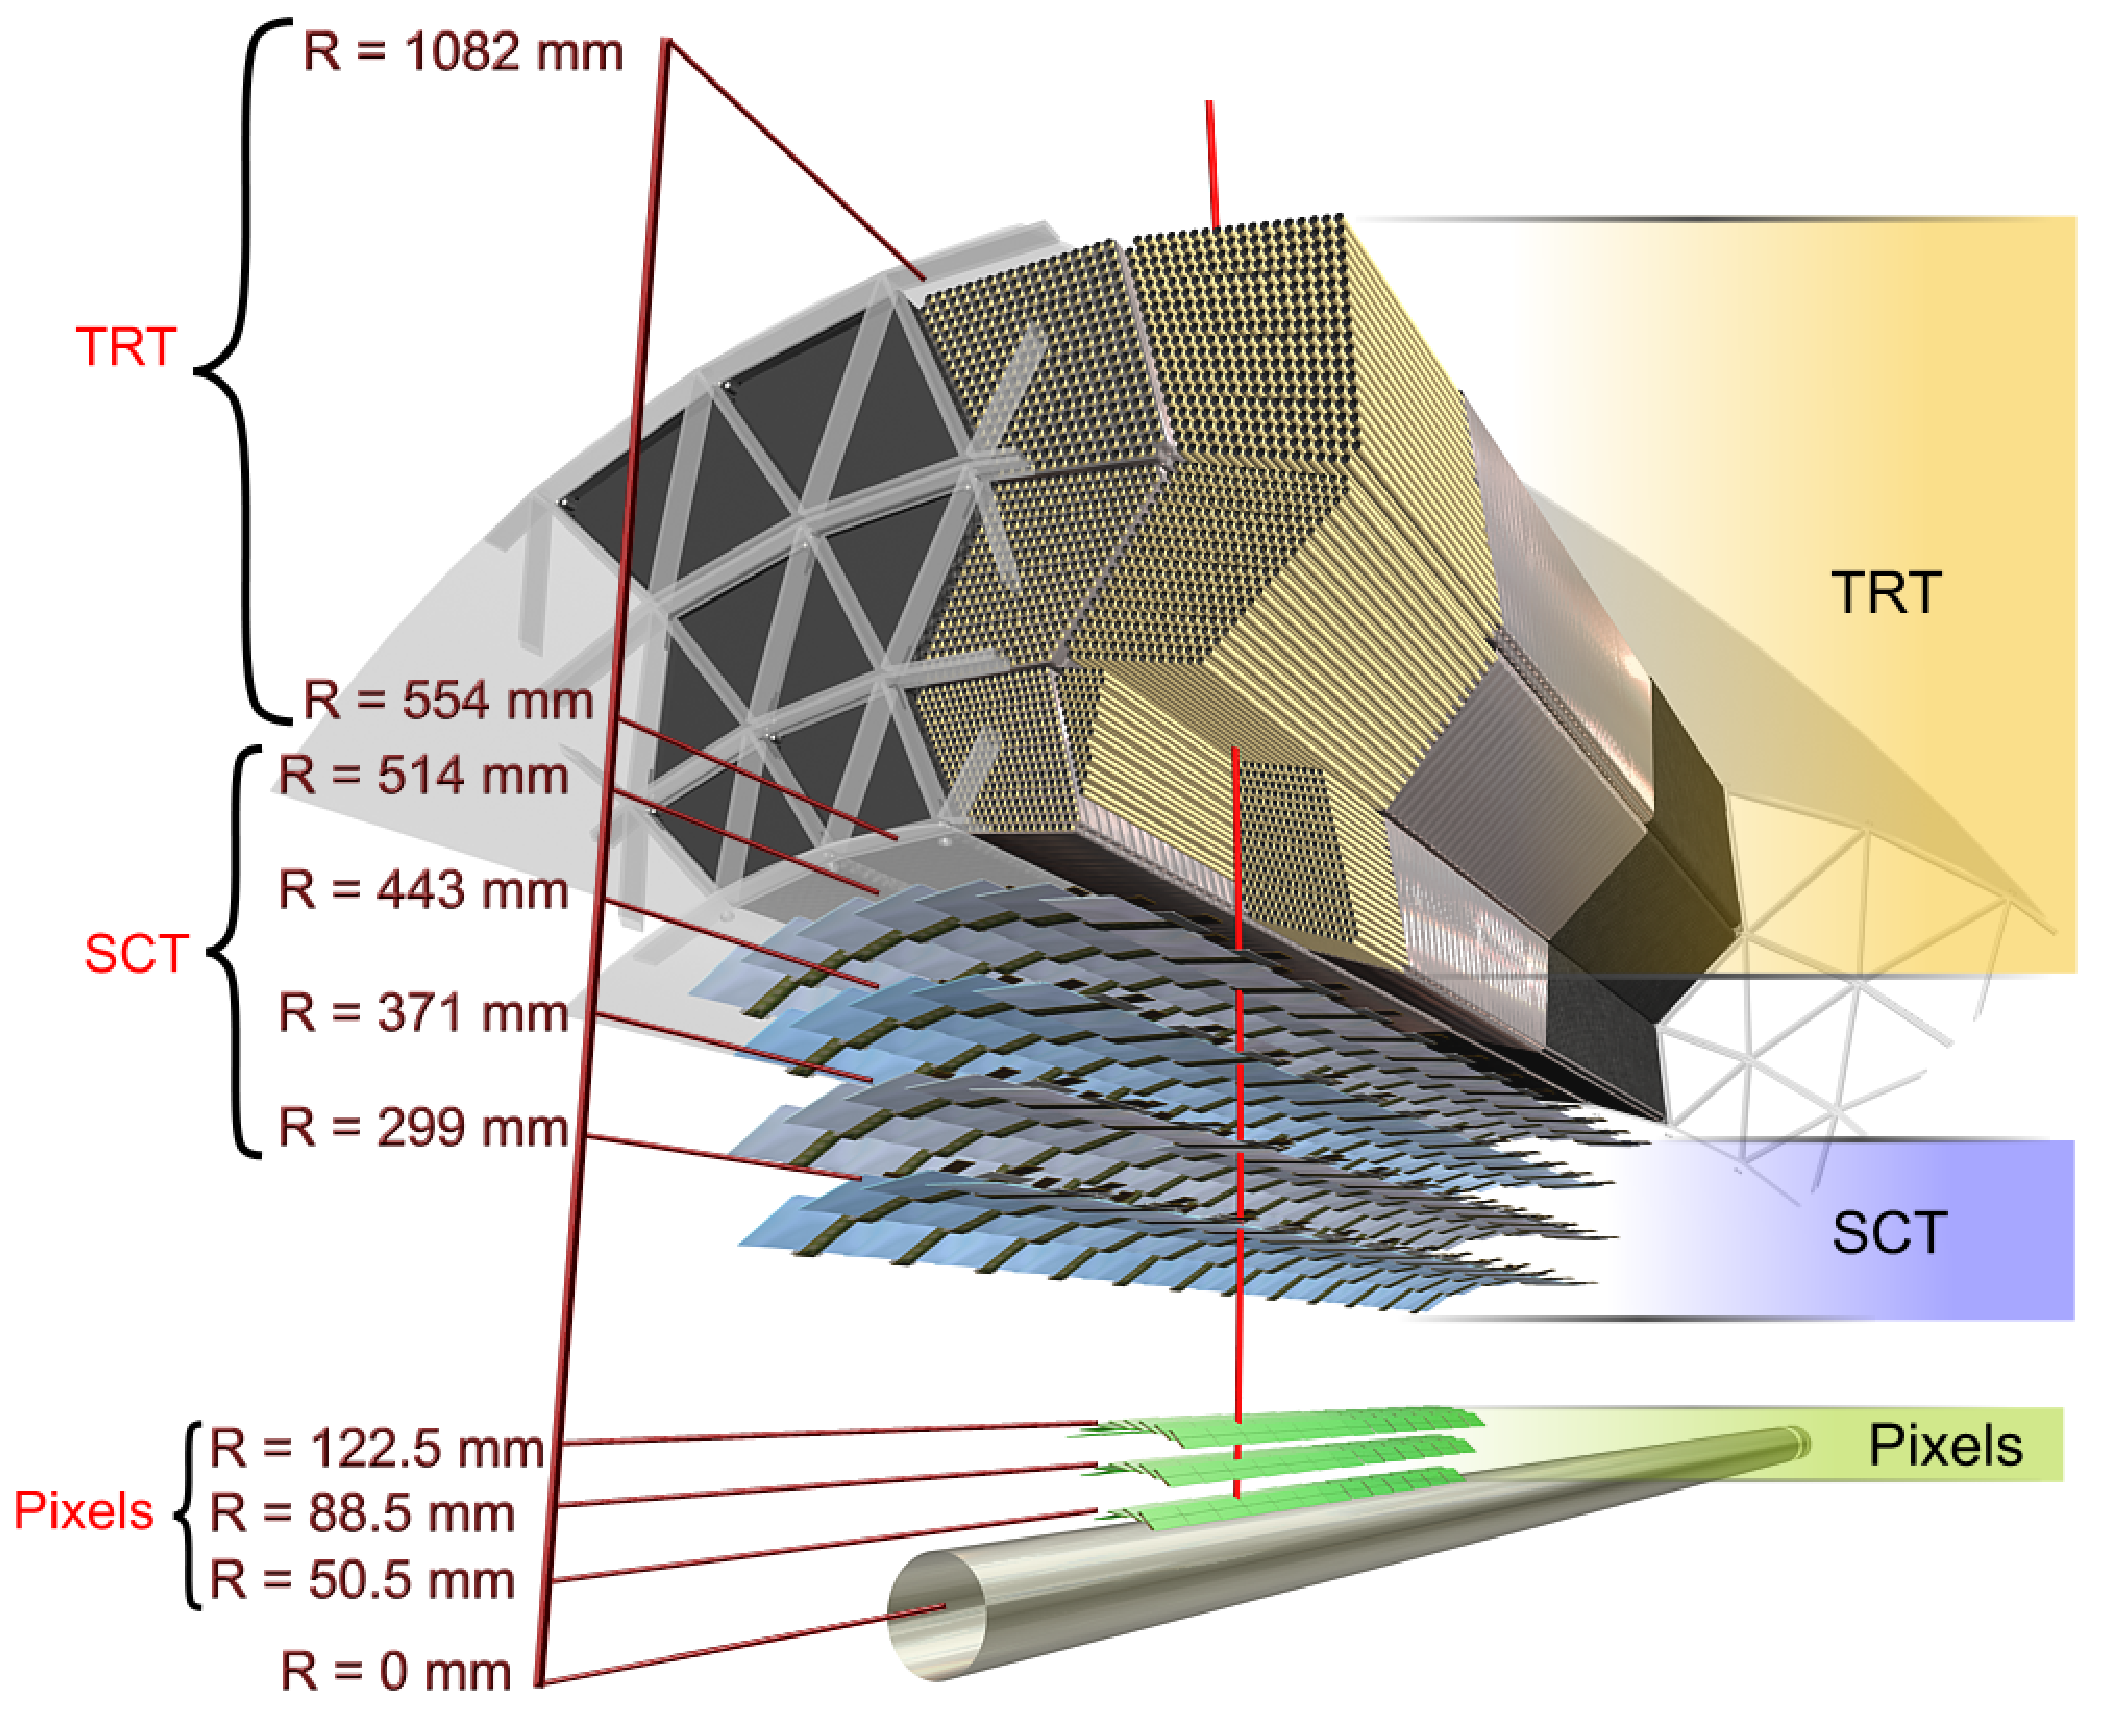
\includegraphics[width=0.8\linewidth,angle=0]{Detector/ID_barrel}
\end{center}
%\centerline{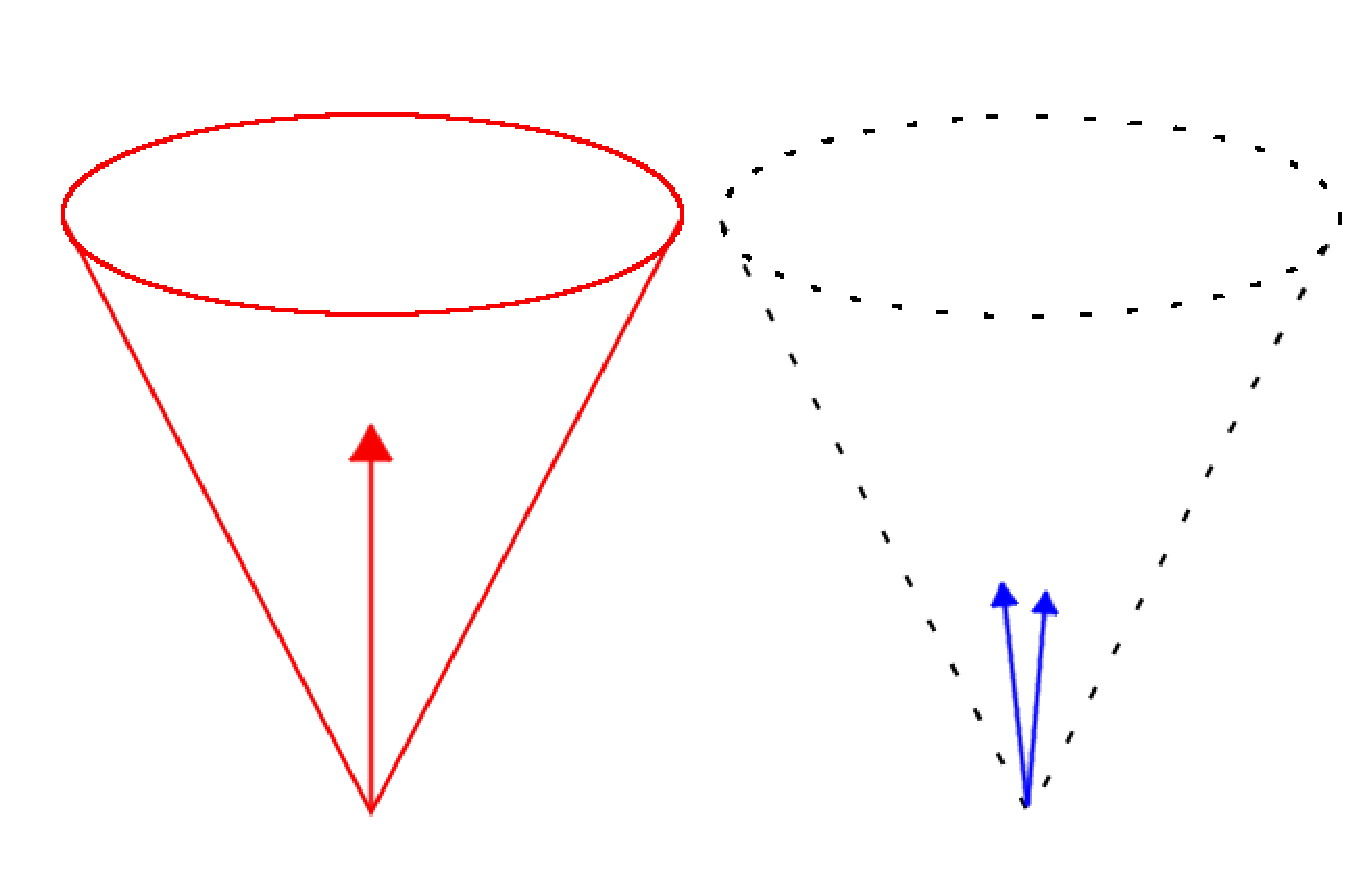
\epsfig{file=./figs/collinear.eps  , width=0.95\textwidth}}
\caption{Diagram of the barrel section of the inner detector.}
\label{fig_ID_barrel}
\end{figure}

\begin{figure}[p]
\begin{center}
\includegraphics[width=0.6\linewidth,angle=0]{Detector/ID_endcap}
\end{center}
%\centerline{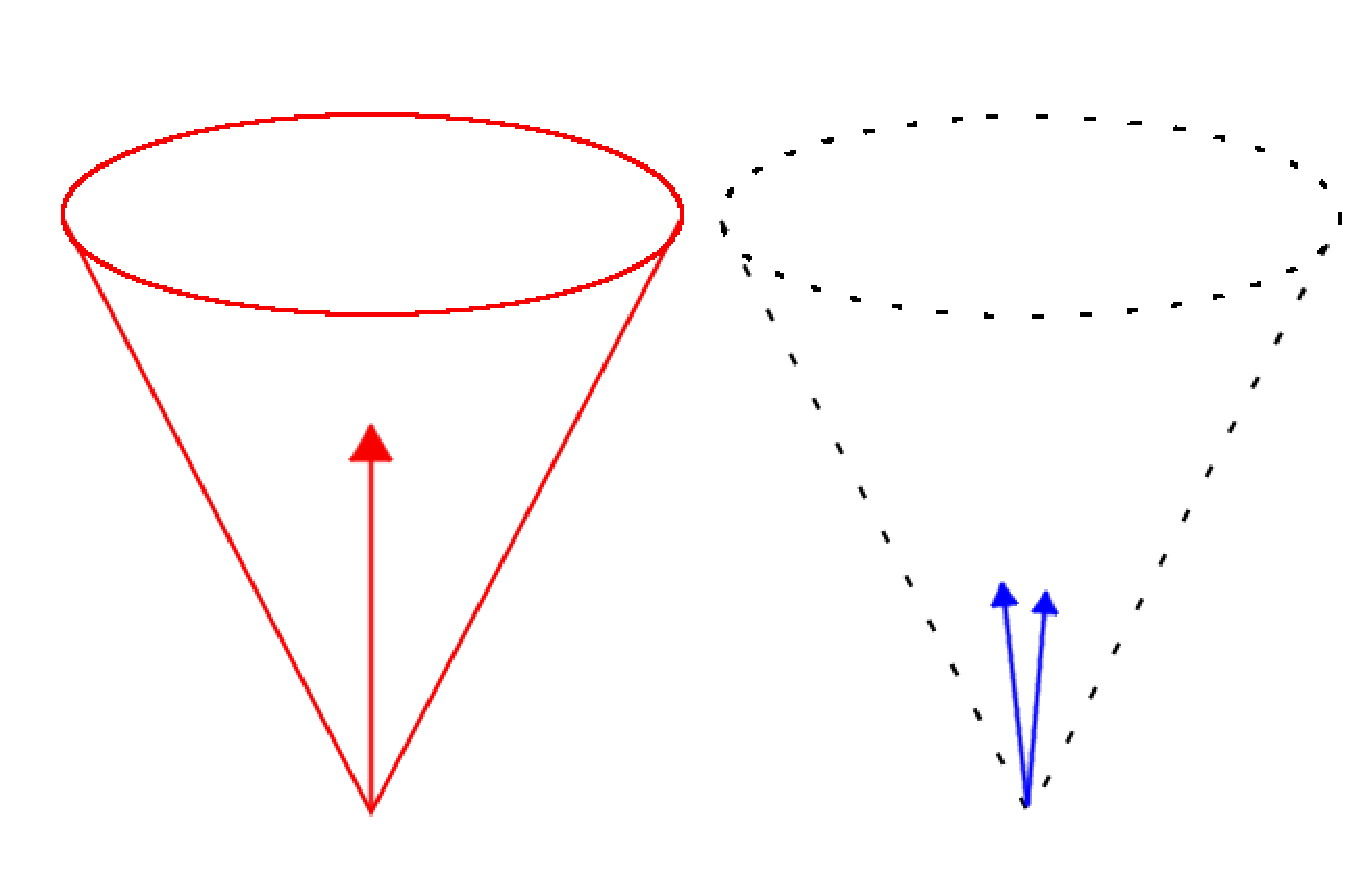
\epsfig{file=./figs/collinear.eps  , width=0.95\textwidth}}
\caption[Diagram of the inner detector]{Diagram of the inner detector, showing the elements traversed by particles at pseudorapidities of 1.4 and 2.2.}
\label{fig_ID_EC}
\end{figure}
%Each component of the inner detector is comprised of one barrel and two end-cap sections, as shown in figure~\ref{}

The pixel detector uses sensors formed from 250$\mu$m thick wafers of silicon. The barrel section consists of three cylindrical layers, and three disc-like layers are used to form each end-cap. All together there are $\sim 8 \times 10^7$ pixel channels, which are designed to provide a hit resolution of 10 $\mu$m in the $R-\phi$ plane and 115 $\mu$m in the $z$ direction in the barrel section. \cmt{something about radiation hardness}

The SCT is located beyond the pixel detector, and consists of 4 cylindrical layers in the barrel section and 9 disc layers in each end-cap. Each SCT module has semiconducting microstrip sensors mounted on both sides that are oriented at an angle of 40 mrad to each other. As a single microstrip sensor only provides a position measurement in one dimension, orienting two at a slight angle allows the position of the hit to be measured in two dimensions, by correlating hits in the two sensors. The SCT is designed to have a resolution of 17 $\mu$m in the $R-\phi$ plane and 580 $\mu$m in $z$.

The TRT is the outermost section of the inner detector, and is formed from straw-shaped drift tubes. The barrel section contains $\sim$52,500 tubes, while $\sim$123,000 tubes are contained in each end-cap section. Straws are made from layers of polyimide, aluminium, polyurethane and graphite-polyimide. Each straw is 4mm in diameter, with a gold-plated tungsten wire (of diameter 31$\mu$m) located in the centre of the tube that serves as an anode. The gas in the tubes is 70\% Xe, 27\% $\mathrm{CO}_2$ and 3\% $\mathrm{O}_2$. Charged particles entering the tube ionise the gas, with the resulting electrons drifting towards the anode in the centre. Measurement of the electron drift time allows the distance of the particle track from the wire to be determined with a resolution of 130$\mu$m. 
The straw tubes are housed within a volume filled with $\mathrm{CO}_2$ and a matrix of polypropylene fibres (in the barrel section) or foils (in the end-caps). Electrons moving between the $\mathrm{CO}_2$/polypropylene interfaces emit transition radiation. This radiation (and the original electron) will then ionise the gas inside the tubes, inducing a signal on the tube anodes. Xenon is used because it efficiently absorbs the transition radiation photons, emitting photoelectrons in the process. Charged pions produce less transition radiation than electrons, and thus generate smaller signals. This difference in signal size allows the TRT to perform particle identification, discriminating electrons from charged pions.

%\red{Inner detector can also determine the vertex of the collisions and shit.}
%provides resolution (distance from wire) of 130 $\mu$m 

%27% CO2, 3%O2 70% Xe


%also used to reconstruct vertices
%
%The pixel detector is innermost, consists of X layers containing Y channels. Resolution of X $\mu$m.
%Consists of layers of semiconducting silicon wafers.
%
%
%n type silicon wafers, oxygenated in order to improve radiation tolerance. Pixel is right next to the IP, so it needs to be radiation hard, to last 10 years or so.
%
%
%
%SCT lies beyond the pixel, covering (dimensions in xyz / eta phi). Consists of 4 cylindrical layers in the barrel section and 9 disks in each side of the end-cap.
%sort out what exactly the stereo deal is.
%
%inner detector covers up to 2.5, tracks charged particles
%
%
%pixel, SCT, TRT
%pic
%
%pixel has X number of strips, dimensions, channels, resolution
%
%SCT, semiconductor tracker (?)
%
%TRT transition radiation tracker - how does this work (exactly)?
%
%
%materials/gasses




%I know nothing about the inner detector
%
%good fig on page 56 of detector paper
%
%ID coverage up to |eta|< 2.5
%electron id for |eta < 2.0, 0.5 GeV < E < 150 GeV
%
%+- 3512mm, r = 1150mm
%solenoid field 2T
%
%pixel, SCT, TRT (dimensions on p55 of Detector paper)
%innermost pixel replaced every three years of running at design luminosity
%3 layers of pixel, 4 layers of SCT
%
%
%
%pixel
%250um thick, ``oxygenated n-type wafers"



%\clearpage
\subsection{Muon Spectrometer}

The Muon Spectrometer is the outermost system of the \atlas detector, and is illustrated in Figure~\ref{fig_Muon_bits}. It is designed to measure muons in the region $|\eta| < 2.7$ with a momentum resolution of $\sim 10\%$ at 1 TeV. However, during 2010 running muons were measured with a resolution of $\sim 5\%$ at 100 GeV in the barrel region\cite{muon_bs}: when the fit to this data is extrapolated, it corresponds to a resolution of $\sim$25\% at 1 TeV. The Muon Spectrometer is also capable of triggering on muons in the region $|\eta| <2.4$. The Muon Spectrometer is comprised of four types of detectors: Monitored Drift Tubes (MDTs), Cathode Strip Chambers (CSCs), Resistive Plate Chambers (RPCs) and Thin Gap Chambers (TGCs). The MDTs and CSCs are referred to as ``precision chambers'' and are used to measure the kinematics of muons, while the TGCs and RPCs are used for triggering and measuring the $\phi$ coordinates of muon tracks.

\begin{figure}[tb]
\begin{center}
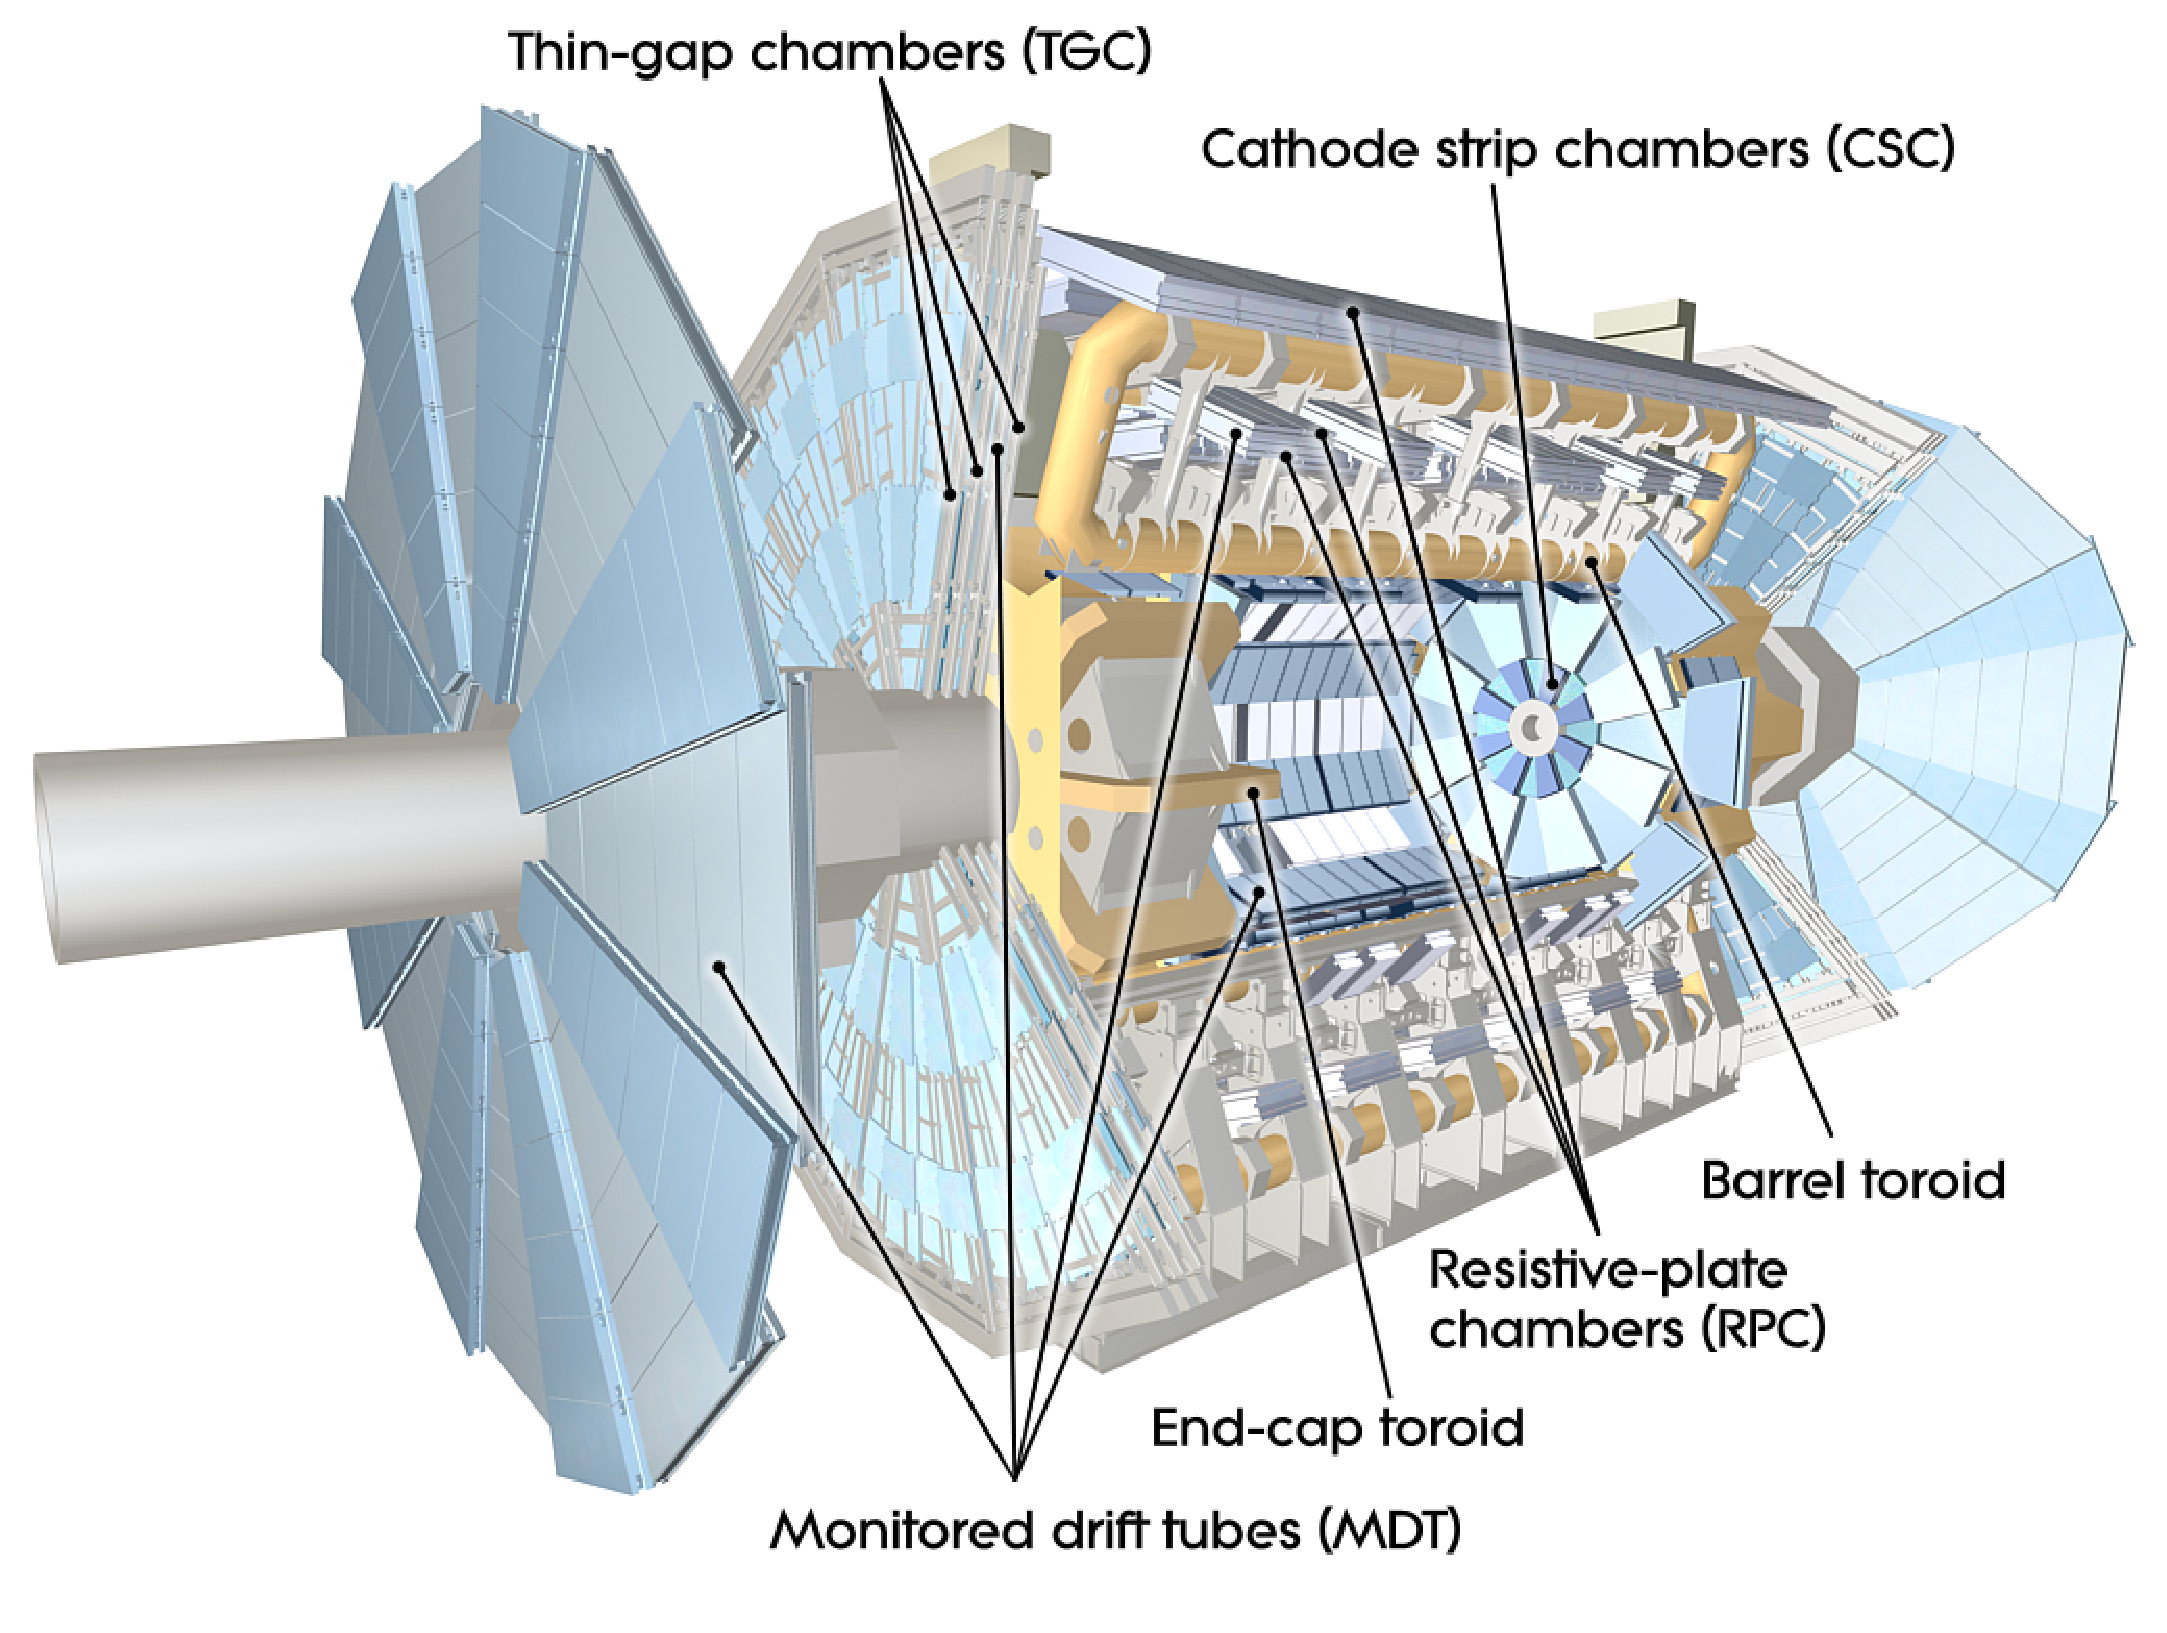
\includegraphics[width=0.8\linewidth,angle=0]{Detector/Muon_bits}
\end{center}
%\centerline{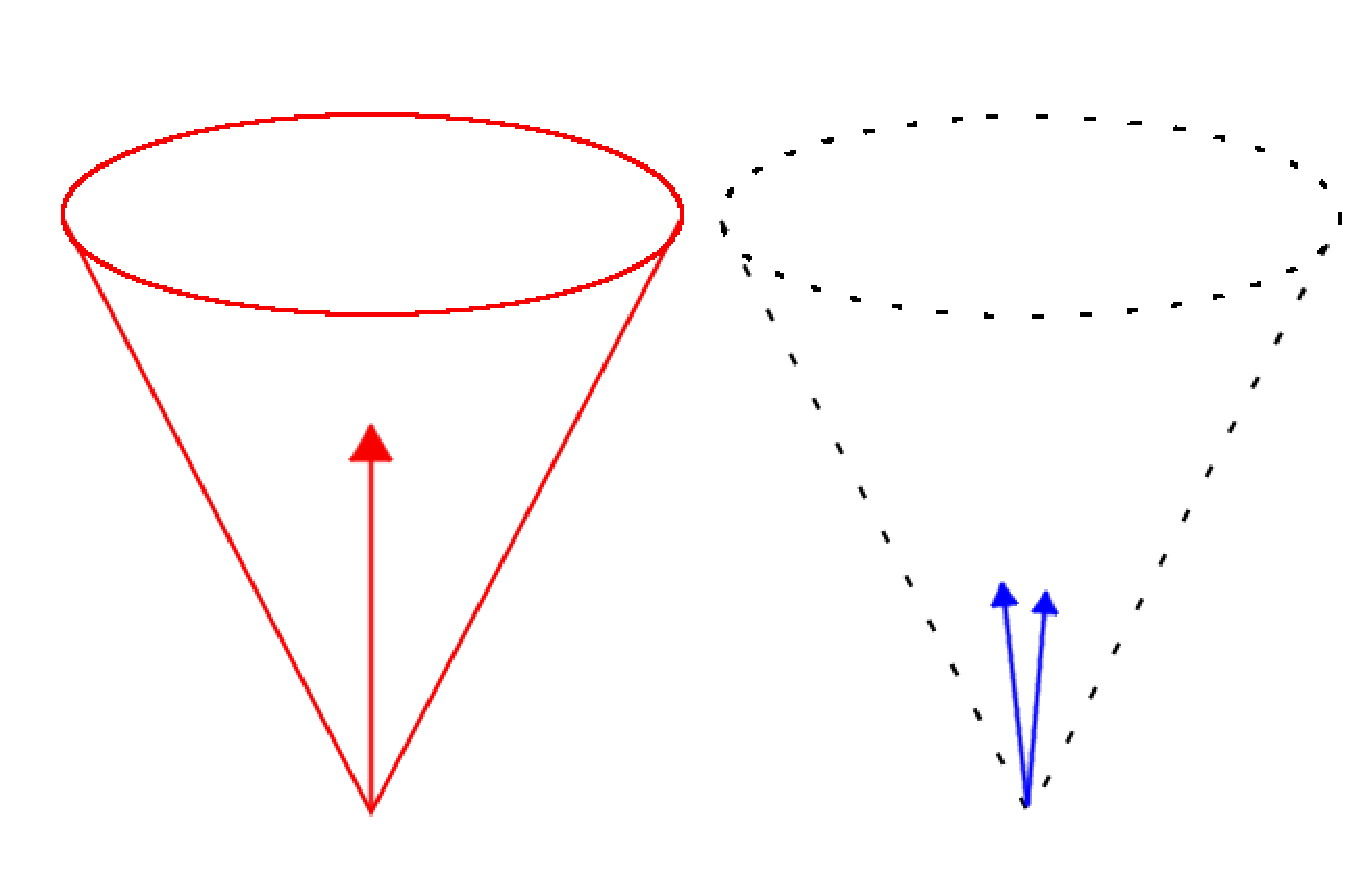
\epsfig{file=./figs/collinear.eps  , width=0.95\textwidth}}
\caption[Components of the Muoin Spectrometer.]{The different components of the Muon Spectrometer. The MDT and CSC components are used for measuring muon momenta, while the RPCs and TGCs are used primarily for triggering.}
\label{fig_Muon_bits}
\end{figure}


Superconducting toroidal magnets (the barrel toroid and two end-cap toroids) are located beyond the calorimeters. 
These produce a toroidal field (i.e. one in which the field lines run in the azimuthal direction), which causes charged particles to bend in the $R-z$ plane. In order to measure track momenta with high resolution, the relative alignment of the MDT and CSC chambers must be well known. A high precision optical system is used to monitor the positions and mechanical deformations of the measurement chambers, which must be known to within 30 $\mu$m in order to achieve the desired momentum resolution.

MDTs are comprised of cylindrical drift tubes of diameter 29.97mm, with a central anode wire of diameter 50$\mu$m. A mixture of Argon (93\%) and $\mathrm{CO}_2$ (7\%) is used to fill the tubes. Each drift tube is capable of measuring the distance of a muon track from the anode wire with a resolution of 80$\mu$m. The tubes are grouped together to form chambers. There are three (roughly) cylindrical layers of chambers in the barrel (at radii of 5 m, 7.5 m and 10 m), and four layers in each end-cap.

%tubes are grouped together into chambers. Three layers of chambers in the barrel section, and two layers in each end-cap


MDTs are used in all four layers of the end-cap sections. However, in the forward region ($|\eta | > 2.0$) of the innermost layer (located at $z \approx 7.4$ m) CSCs are used instead, as the MDTs are unable to operate in the high levels of radiation present in this region. The CSCs are multi-wire proportional chambers (MWPCs), filled with a mixture of Argon (80\%) and $\mathrm{CO}_2$ (20\%), and are capable of measuring hit positions to within 60 $\mu$m in the bending plane.

For triggering purposes, RPCs are used in the barrel region ($|\eta| < 1.05$) while TGCs (which are a form of MWPC) are used in the end-cap region ($1.05 > |\eta| > 2.4$). The intrinsic response time of these detectors is on the order of a few nanoseconds, enabling them to reliably identify the bunch crossing in which any detected muons were produced.
\subsection{Calorimetry}

\subsubsection{Sampling Calorimeters}

All of the calorimeters used at \atlas are sampling calorimeters, which consist of active regions and passive (absorbing) regions. The active layers are sensitive: energy deposited in these regions produces a signal which is then read out. The passive regions are made from a denser absorbing material, which is used to regulate the shower size. Sampling calorimeters are less expensive to produce than homogenous calorimeters\cmt{, and tend to occupy less space: If a homogenous calorimeter can completely contain a shower in a given volume, then a sampling calorimeter made using the same active material will be able to contain the shower in a smaller volume}.

 Sampling calorimeters may be characterised by their sampling fraction, which is defined as the energy deposited in the active regions by a minimum ionising particle (MIP) divided by the total energy deposited in the active and passive regions by the MIP~\cite{wigmans2000calorimetry}.
%
%calorimeter designs consist of active layers and a passive layers of absorbing material. Absorbing material dense, there to reduce shower size, active layers sensitive: energy deposited in these regions produces a signal that is read out.

Most of the \atlas calorimeters are based on liquid argon (LAr) technology, i.e. LAr is used to form the active regions of the calorimeter. Charged particles passing through these active regions ionise the liquid argon. The liberated electrons then drift in an applied electric field, resulting in an induced current pulse. This current is then used as a signal.

The \atlas Tile calorimeter uses tiles of scintillating polystyrene as the active material. These are positioned between layers of steel (the passive material). Charged particles passing through these tiles excite the scintillating material, which then produces photons. This scintillation light is then wavelength shifted in order to prevent it from being reabsorbed by the scintillating material, and then carried by optical fibres to photomultiplier tubes (PMTs), which absorb the light and produce an electrical signal.

%Sampling fraction. defined as the visible (signal-producing) energy deposited in active region divided by the total energy deposited in the calorimeter.
%Sampling calorimeters are characterised by their sampling fraction, which is defined as the total energy  


\subsubsection{Electromagnetic Shower Development}

Photons and electrons interact with the calorimeter via electromagnetic (EM) processes. The dominant processes by which electrons (or positrons) lose energy while traversing the material of the calorimeter are ionisation and Bremsstrahlung. At high energies Bremsstrahlung dominates, while at lower energies ionisation is the dominant process. The critical energy, $\epsilon_c$, is defined as the value of an electron's energy at which the rate of energy loss via ionisation is equal to the rate of energy loss from Bremsstrahlung. This value  is material dependent, but an approximation for solids and liquids is given by\cite{wigmans2000calorimetry}

\begin{equation}
\epsilon_c = \frac{610 \mathrm{MeV}}{Z + 1.24}
\end{equation}
where $Z$ is the atomic number of the element being traversed.

The longitudinal extent of an EM shower may be expressed in terms of the radiation length, which is the distance over which an electron loses $\sim63\%$  ($1- e^{-1}$) of its energy via Bremsstrahlung. The radiation length of a material may be approximated by\cite{ReviewPP98}
\begin{equation}
X_0 = \frac{716.4 \,A }{Z(Z+1) \log(287/\sqrt{Z})} \quad \mathrm{g cm}^{-2},
\end{equation}
where $Z$ is the atomic number of the element. Note that the expression has units of $\mathrm{g~cm}^{-2}$, and so should be divided by the density of the material in order to obtain a value with dimensions of length. In cases where the material is comprised of multiple elements, then the radiation length of the compound is given by
\begin{equation}
\frac{1}{X_0} = \sum_j \frac{w_j}{X_{0,j}},
\end{equation}
where the $X_{0,j}$ and $w_j$ are, respectively, the radiation length and fraction (by mass) of the $j$-th element.

A similar quantity exists to describe the lateral extent of an EM shower. The \moliere radius, $\rho_M$, is given by 
\begin{equation}
\rho_M = X_0 \frac{21.2 \mathrm{MeV}}{\epsilon_c}.
\end{equation}
Unlike the radiation length, the \moliere radius doesn't have a strict physical meaning, although roughly $80-90\%$ of an EM shower's energy is generally deposited within a cylinder of radius $\rho_M$~\cite{wigmans2000calorimetry}.


The dominant processes for photons are pair production, Compton scattering and the photoelectric effect. At higher energies ( $  \gtrsim 10$ MeV) pair production is the most likely, though as the photon's energy decreases Compton scattering becomes more prevalent, while the photoelectric effect dominates at the lowest energies ( $\lesssim 1$ MeV). The average distance that a high energy photon travels before undergoing pair production is 9/7 $X_0$.

Typically, EM showers consist of successive Bremsstrahlung and pair production interactions. An initial electron will radiate, producing a photon. The photon will then undergo pair production, yielding an electron-positron pair in addition to the original electron. This process then repeats, with electrons and positrons radiating photons that then convert into additional electron-positron pairs. This continues until the electron/positron energies fall below the critical energy, at which point they are more likely to lose energy via ionisation than through further radiation. The energy of the initial electron is thus divided between all the electrons and photons produced during the shower, with the electrons then depositing their energy in the calorimeter via ionisation. Ionisation in the active layers of a calorimeter is used to generate a signal: in the LAr calorimeters the ionisation induces a current in the electrode, which is used as a signal, while in the Tile it produces photons via scintillation, which are then guided to a photomultiplier tube and used to produce an electrical signal.
%
% 
% in which the the electric field of the passing electron causes another electron to be ejected from an atom of the material,and Bremsstrahlung radiation. Brems
%
%Electrons passing through a calorimeter will lose energy via Bremsstrahlung radiation or by ionising the calorimeter material. 
%explain these
%
%EM showers characterised by radiation length. For a given material ..
%
%
%radiation length is defined as the average length an electron will travel before losing $63\% (1-e^-1) $of its energy via Bremsstrahlung radiation. an approximation for this is given by 


\subsubsection{Hadronic Shower Development}
\label{detector_had_showers}
While EM showers tend to be dominated by only a few processes, there are many more processes that may take place in a hadronic shower, making them more complex. 

The longitudinal development of hadronic showers is characterised by the nuclear interaction length, $\lambda_\mathrm{int}$, which describes the average distance that a hadron will travel in a material before interacting with a nucleus. In general, $\lambda_\mathrm{int}$ scales as $A^{1/3}$, where $A$ is the mass number of the element being traversed.

Hadronic showers have an EM component and a non-EM component. Of the $\pi$ mesons produced in hadronic interactions, roughly 1/3 are $\pi^0$ mesons. The decay $\pi^0 \rightarrow \gamma \gamma$ occurs very quickly (at rest, the $\pi^0$ has a lifetime of $8.5 \times 10^{-17}$s), with a branching fraction of 99\%~\cite{reviewPP2012}. Thus, almost all the $\pi^0$'s produced in hadronic showers go on to induce EM showers. At each interaction, some of the energy carried by the non-EM component is redirected into the EM component. As the energy of the initial hadron increases, the number of interactions (and thus the fraction of energy carried by the EM component) increases also. The energy carried by the EM component thus scales non-linearly with the energy of the initial hadron. 

A feature of the non-EM component of hadronic showers is that some of the energy deposited in the active layers is invisible to the calorimeter. For instance, when a showering hadron interacts with a nucleus and frees a number of nucleons, the binding energy required to release those nucleons is essentially lost: it is invisible to the calorimeter. Neutrons are produced in large quantities during nuclear interactions, and while these may undergo further nuclear interactions they will not ionise the active region of the calorimeter, and so in that sense are invisible. Furthermore, hadronic interactions with nuclei may produce particles that decay to muons and/or neutrinos. Muons (unlike electrons) deposit a minimal amount of energy via ionisation before leaving the calorimeter, while neutrinos (almost always) leave the calorimeter without interacting at all.

A calorimeter will have a lower response to a hadronic shower than it would to an EM shower of the same initial energy, unless it somehow corrects for this invisible energy. This correction is referred to as compensation.
%  Compensation may be achieved by boosting the response to the non_em component of the shower, diminishing the EM response, or both. 
 The most effective way to achieve compensation is by increasing the calorimeter's response to the non-EM shower component. This response may be boosted if the active material contains hydrogen (as is the case with scintillating materials). In this case, the neutrons produced in nuclear interactions can scatter off hydrogen nuclei. The active material is then sensitive to the recoiling proton~\cite{wigmans2008calorimetry}. Alternatively, using fissile material as an absorbing material can boost the non-EM response. Energy released in fission reactions can compensate for invisible energy losses. The ZEUS\cite{zeus} calorimeter is based on uranium/scintillator technology, and is an example of a compensating calorimeter.\cmt{However, most of the energy released in fission carried by neutrons, so still need H in the active material.}
 
 
% nuclear interaction length, lambda_int, average distance hadrons travel before having a nuclear interaction. scales as A^1/3 (mass number)
  
The \atlas calorimeters are all non-compensating, and thus the response of the calorimeters to hadrons is lower than for electrons of the same energy. Software-based methods are used during offline reconstruction to correct for this effect, as described in sections~\ref{section_TB_hadron_results} and~\ref{section_JES}

\subsubsection{Calorimeter Energy Resolution}

%fluctuations. certain things can cause variations in the measured energy. 
The performance of a sampling calorimeter may be characterised in terms of its resolution, $\sigma/\bar{E}$, where $\bar{E}$ is the mean reconstructed energy and $\sigma$ is the RMS of the calorimeter response. The resolution is typically parameterised by a function of the form
\begin{equation}
\frac{\sigma}{\bar{E}} = \frac{A}{\sqrt{\bar{E}}} \oplus B \oplus \frac{C}{\bar{E}},
\label{eqn_resolution_general}
\end{equation}
where $A$, $B$, and $C$ are called the stochastic, constant, and noise terms, respectively, and $\oplus$ denotes addition in quadrature.

The stochastic term arises from variations in the sampled energy, for example, an incident particle may shower in a way that deposits a large amount of energy in the active regions of the calorimeter, or in a way that deposits less energy in these regions. These sampling fluctuations are governed by Poisson statistics, and thus give rise to a term proportional to $\bar{E}^{-1/2}$ in the resolution\cite{fabiola_calorimetry}.

The constant term arises from effects that are independent of energy deposited in the detector, such as non-uniformities in the calorimeter response. These non-uniformities may be caused by uninstrumented material in front of the calorimeter, irregularities in the calorimeter structure, or damage caused by radiation or aging, or a calorimeter design in which the response is dependent on the impact point of the incident particle. This impact point dependence forms the dominant contribution to the constant term for the forward calorimeters of \atlas, which is discussed further in section~\ref{TB_results_electrons}.

The noise term is associated with electronic noise in the readout chain. For the liquid argon calorimeters used at \atlas, the majority of this noise is introduced in the preamplifiers which are located on the front end boards. The noise contribution is independent of the signal being read out of the channel, and so the noise term in the resolution scales as $\bar{E}^{-1}$.


%Sampling calorimeter performance characterised by its resolution, sigma/e, where E is the mean reconstructed energy and sigma is the rms of the calorimeter response.
%
%calorimeter resolution may typically be parameterised by a function of the form
%
%
%A, B and C are the stochastic, constant, and noise terms, respectively, and $\oplus$ denotes that the terms should be added in quadrature.
%
%stochastic term arises from variations in the sampled energy, that is, incident particle may shower in a way that deposits a large amount of energy in the active regions of the calorimeter, or in a way that deposits less energy in these regions. these fluctuations are governed by Poisson statistics, and thus give rise to a term proportional to 1/sqrt E in the resolution.
%
%noise term - electronic noise in the readout chain. For the liquid argon calorimeters discussed below, the majority of this noise is introduced in the preamplifiers. noise independent of the energy  being read out from a given channel, and so contribution to the resolution proportional to 1/E
%
%constant term - energy independent things, like detector nonuniformities, etc. 
%
%
%Sampling calorimeters typically have 
%X0 =
%
%ec?

%length scale that characterises longitudinal development of EM showers.
%radiation length describes the mean distance that an electron travels before 
%
%Also, there is the Moliere radius
%
%describes the lateral development.
%
%
%
%
%Fucking Wigmans motherfucker
%
%or Em shower development
%
%hadronic shower development
%
%sampling calorimeters
%
%
%
%sampling calorimeters
%sampling fraction
%
%Em showers
%brems, pair production
%radiation length, Moliere radius
%
%hadronic showers
%invisible energy
%compensation
%(E dependence of EM component)
%
%
%hadronic showers
%
%hadronic showers deposit less visible energy in calorimeter than EM showers

\subsection{The ATLAS Calorimeters}



%The precision electromagnetic calorimeters are lead-liquid0
\atlas contains five distinct calorimeters, shown in Figure~\ref{fig_calorimeters}. The Electromagnetic Barrel (EMB) Calorimeter is located in the central ``barrel'' section of \atlas, while the Electromagnetic End-cap Calorimeter (EMEC), Hadronic End-cap Calorimeter (HEC) and Forward Calorimeters (FCal) are located within the end-caps at either end. The Tile calorimeter consists of barrel section, and two extended barrel sections that surround the end-cap cryostats.
\begin{figure}[tb]
\begin{center}
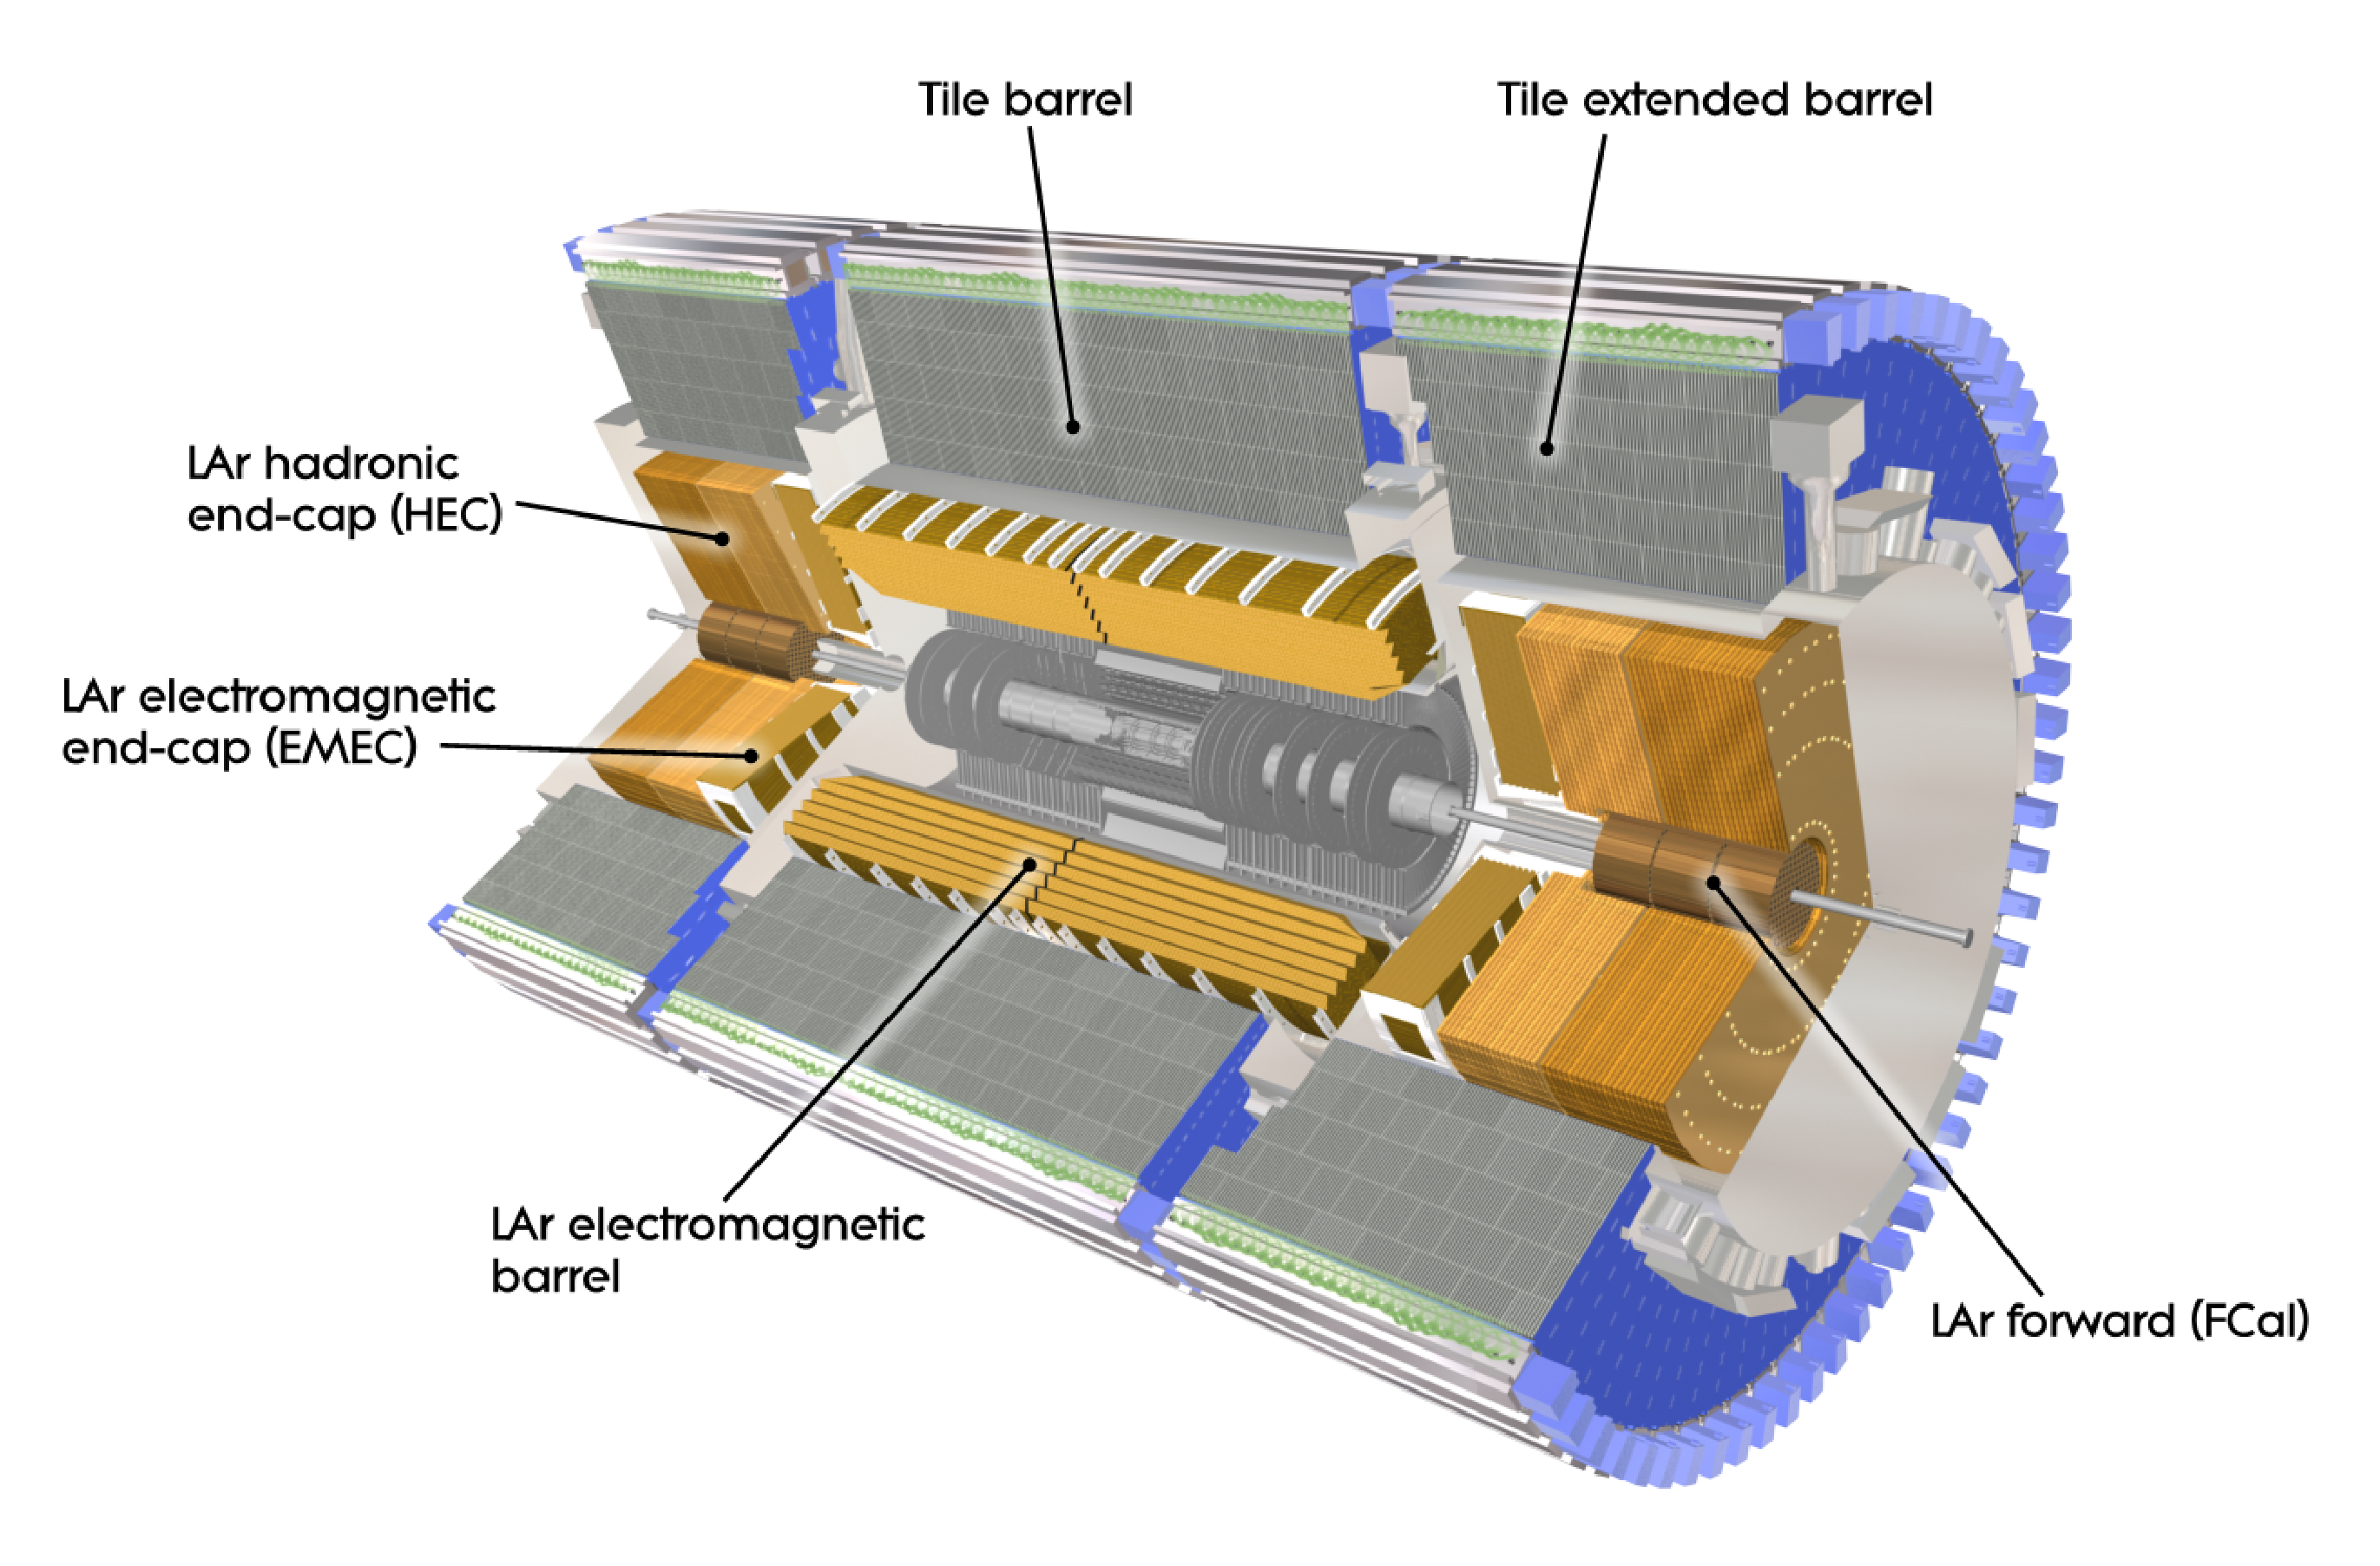
\includegraphics[width=0.8\linewidth,angle=0]{Detector/calorimeters}
\end{center}
%\centerline{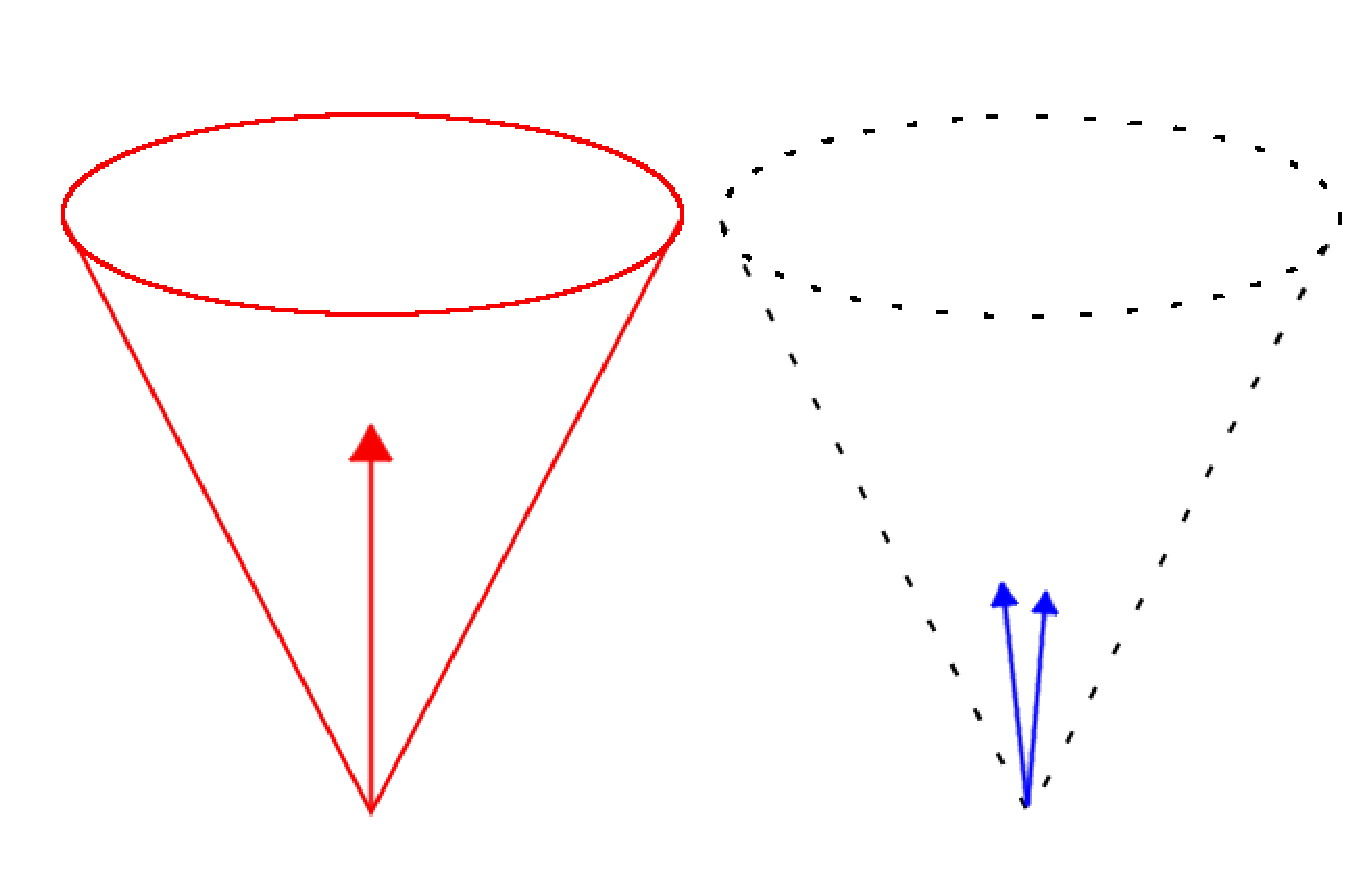
\epsfig{file=./figs/collinear.eps  , width=0.95\textwidth}}
\caption{The calorimeters of the ATLAS detector.}
\label{fig_calorimeters}
\end{figure}
\subsubsection{Barrel Calorimeters}
%\red{All these calorimeters use liquid argon as the active detector medium; liquid argon has been chosen for its intrinsic linear behaviour, its stability of response over time and its intrinsic radiation-hardness. }

%\red{ok, need to discuss why LAr is used, and why its accordion shaped}
%The EM Barrel (EMB) calorimeter is a lead/liquid argon calorimeter covering the ps with a distinctive accordion-shaped geometry. 
%
%
%It is made up of two half barrel sections ($z < 0$ and $z > 0$), each divided azimuthally into 16 modules. It covers the pseudorapidity range $0< |\eta| < 1.475$, and is completely symmetric in $\phi$.

% consists of three layers, plus presampler. 
The EMB calorimeter is a lead/liquid argon sampling calorimeter covering the pseudorapidity range $|\eta| < 1.475$. Liquid argon \cmt{(LAr)} was chosen for the active medium because it can be used to obtain a fast, linear response while also being resistant to radiation~\cite{detector_paper}. The absorber plates are folded into a distinctive accordion shape, as shown in Figure ~\ref{fig_EMB_section}. The shape of the absorber plates gives the EMB calorimeter a structure that is completely symmetric in the azimuthal direction, with no gaps in detector coverage. The linearity and resolution of the response are thus uniform in $\phi$.


%The absorber plates are made of lead, and are 1.5mm thick for $|\eta| < 0.8$ and 1.1 m thick for $|\eta| > 0.8$.  

The absorber plates are made of lead, with stainless steel sheets glued on each side in order to increase their mechanical strength. The plates are then folded into the accordion shape, with the folding angle increasing with depth (radius) in order to maintain the size of the LAr gap (and hence the sampling fraction) throughout the calorimeter. The lead plates are 1.5mm thick for $|\eta| < 0.8$ and 1.1 m thick for $|\eta| > 0.8$. Thinner sheets are used at higher $|\eta|$ in order to control the depth of the calorimeter\cite{TDR_LAR}, which varies from 22 - 30 $X_0$ in the region $0 < |\eta|<0.8$, and from 24 to 33 $X_0$ in the region $0.8 < |\eta|<1.3$. 

%The depth of the calorimeter increases with $\eta$, as particles at higher values of $\eta$ will travel a longer distance in order to traverse the same radial depth. 
% 
%
%change thickness, reduces depth. More LAr, so better response/resolution
%
%
% An 0.2mm sheet of stainless steel is glued onto each side of the lead plate in order to increase the mechanical strength of the absorber sheets. These sheets are then folded into the accordion shape. The folding angle increases with depth (radius) in order to maintain the size of the LAr gap throughout the calorimeter. 

%, which is 2.1mm on either side of the electrodes.
\begin{figure}[tb]
\begin{center}
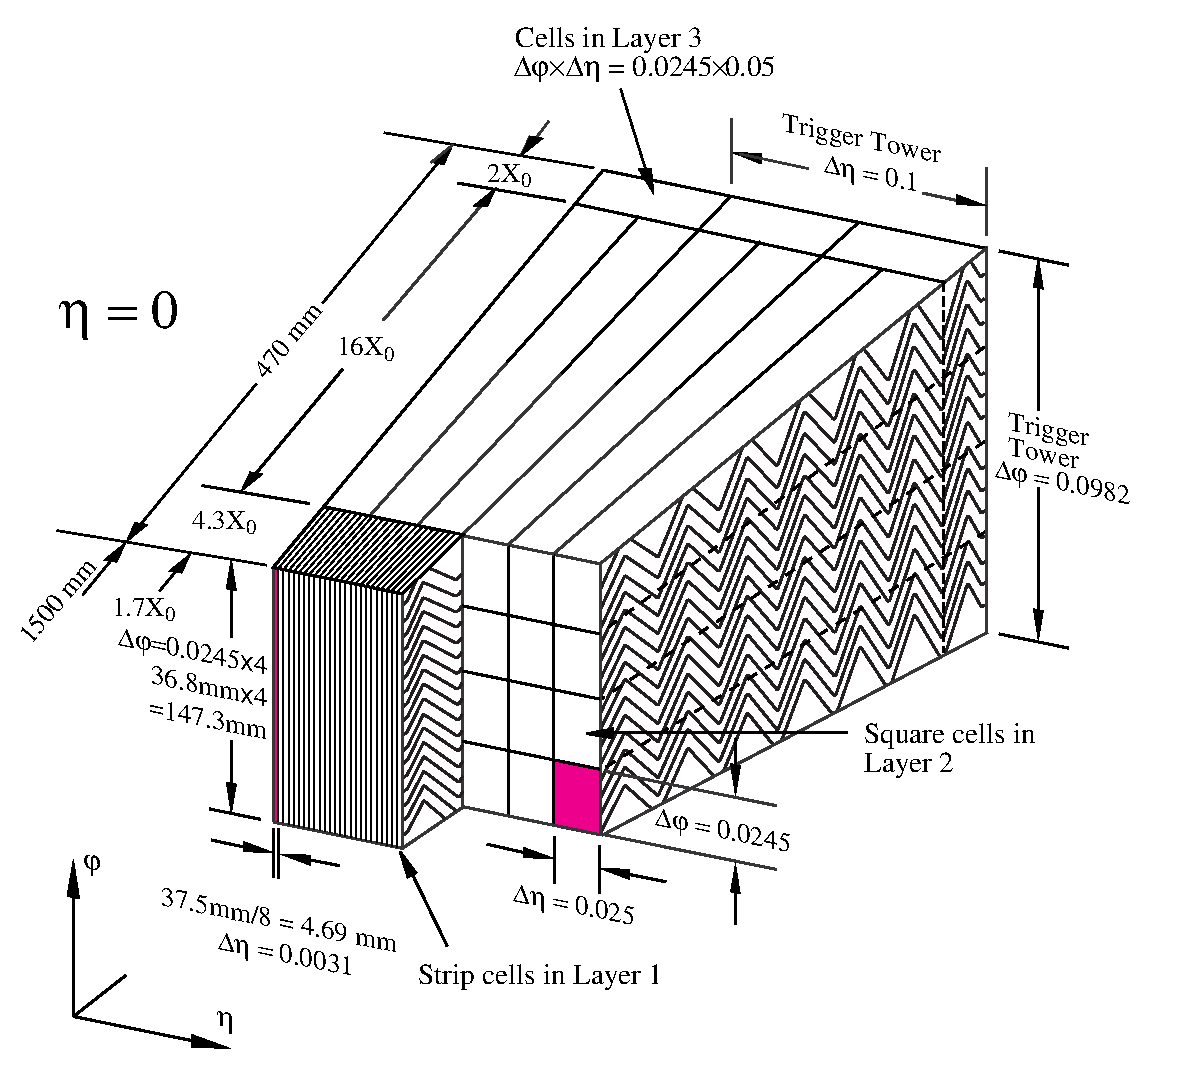
\includegraphics[width=0.5\linewidth,angle=0]{Detector/EMB_section}
\end{center}
%\centerline{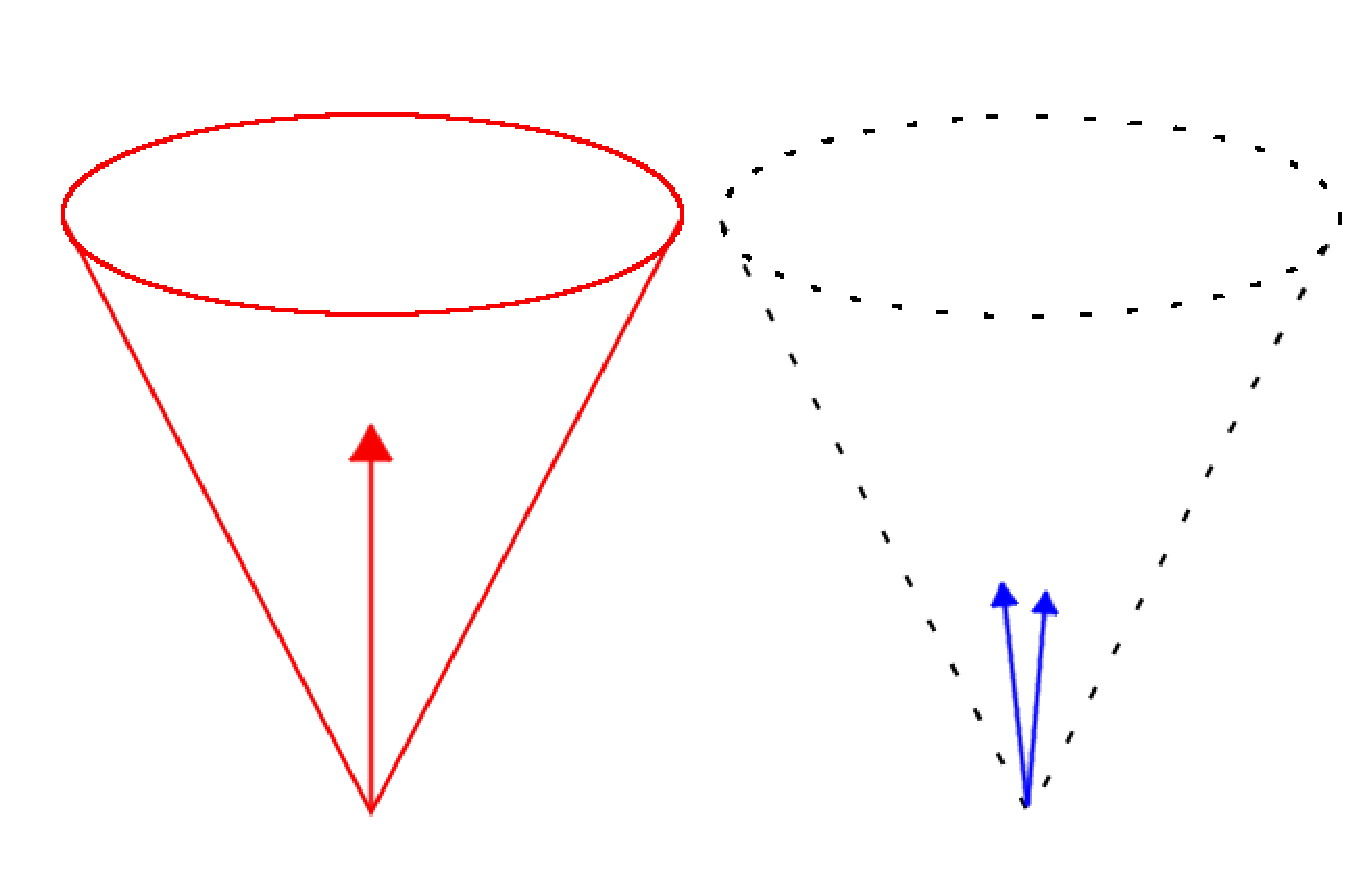
\epsfig{file=./figs/collinear.eps  , width=0.95\textwidth}}
\caption[Section of the EMB calorimeter]{Section of the electromagnetic barrel calorimeter, showing the accordion shape of the absorber plates.}
\label{fig_EMB_section}
\end{figure}

Flexible Printed Circuit Boards (PCBs) are used to form the electrodes, which consist of three layers of copper separated by polyimide. The electrodes are positioned in between layers of the absorber, with honeycomb spacers being used to keep the electrodes in the centre of these gaps. The absorber layers are grounded, while the two outer layers of copper on each electrode are connected to an HV supply at +2kV~\cite{detector_paper}. This creates two active liquid argon gaps of thickness 2.1 mm on either side of the electrode. The inner layer of copper on each electrode is used to read out the signal, as it is capacitively coupled to both the outer layers.


The readout of the EM Barrel calorimeter~\cite{ATLAS_barrel_electrode} is divided longitudinally (i.e. in depth) into three layers. The first and third layers are each a few $X_0$ in depth and only contain the beginning and end of the shower, while most of the energy is deposited in the second layer which has a depth of $\sim$17-20 $X_0$. The readout granularity in $\Delta \eta \times \Delta \phi$ is 0.003 $\times$ 0.1, 0.025 $\times$ 0.0245, and 0.05 $\times$ 0.0245 in layers 1, 2 and 3, respectively. A diagram of the readout layer of the electrode is shown in Figure~\ref{fig_EMB_electrode}, in which the different readout granularities are visible. The first layer has a very fine segmentation in $\eta$, which allows decaying $\pi^0$ particles to be distinguished from individual photons.\cmt{cite tdr}

\begin{figure}[tb]
\begin{center}
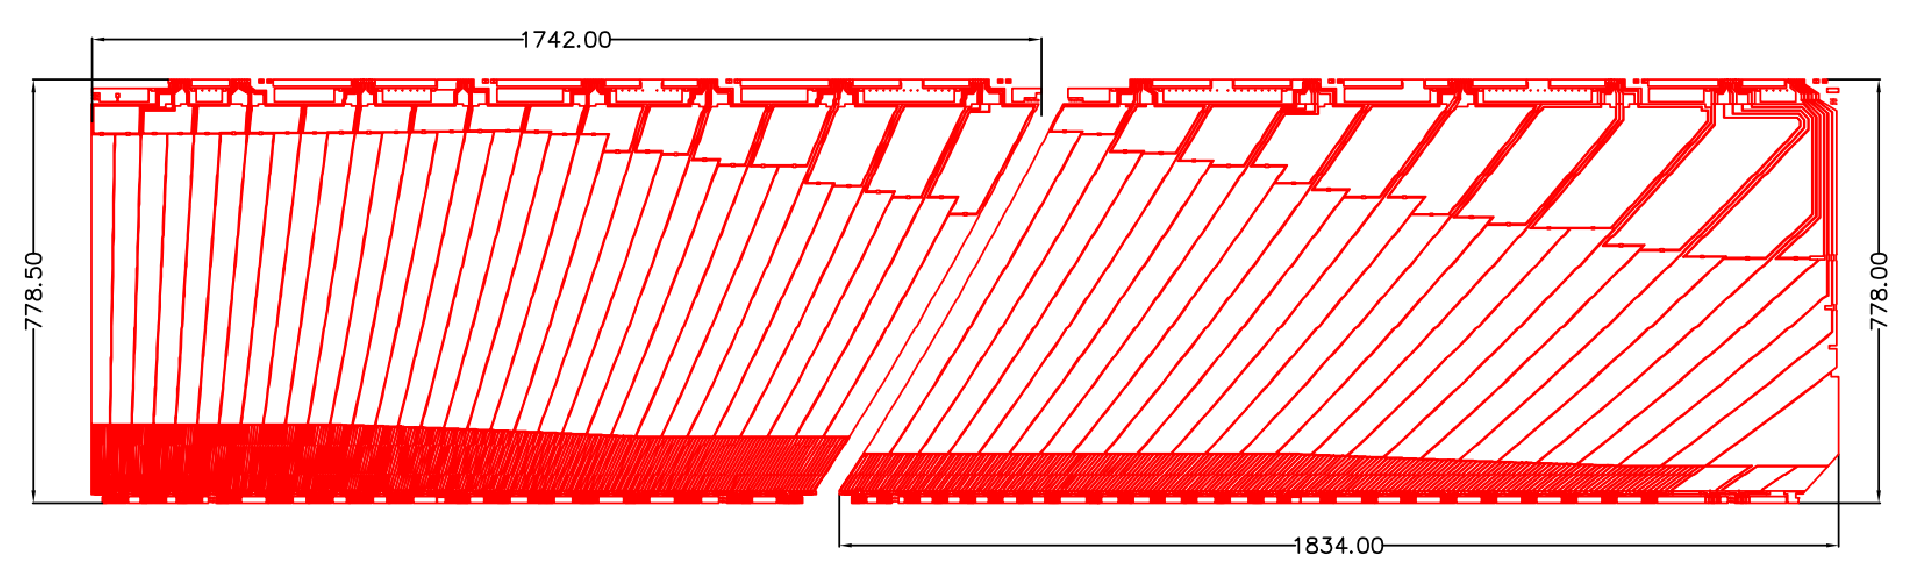
\includegraphics[width=0.95\linewidth,angle=0]{Detector/EMB_electrode}
\end{center}
%\centerline{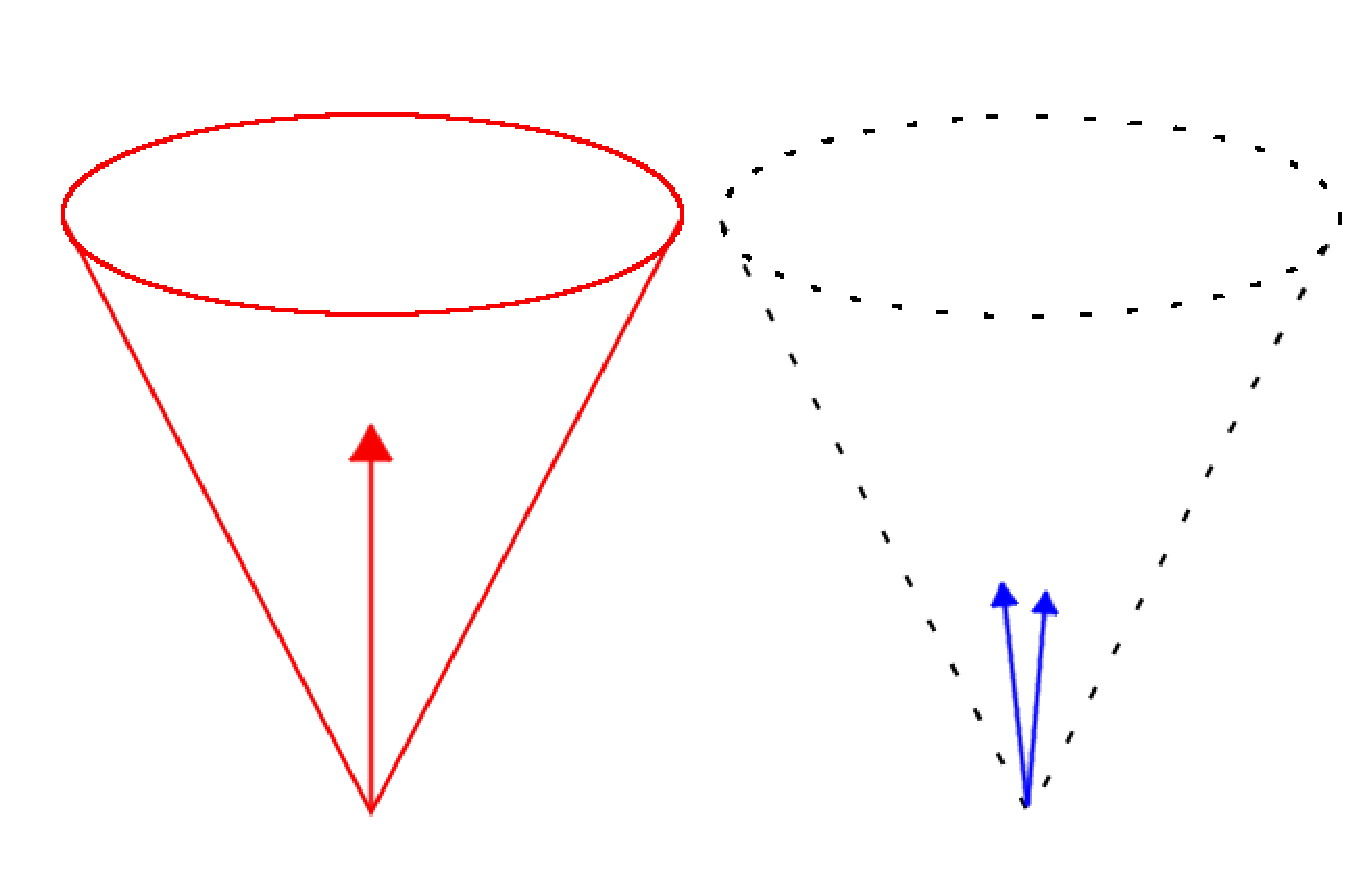
\epsfig{file=./figs/collinear.eps  , width=0.95\textwidth}}
\caption[Readout layer of EMB electrode]{Schematic view of the readout layer of an EM Barrel electrode, prior to folding. The piece on the left is used to read out signals from $0 < \eta < 0.8$, while the piece on the right covers the region $0.8 < \eta < 1.475$~\cite{ATLAS_barrel_electrode}.}
\label{fig_EMB_electrode}
\end{figure}






%TILE
%\red{The choice of this technology provides maximum radial depth for the least cost for ATLAS}
A steel/scintillator ``Tile'' calorimeter~\cite{ATLAS_TILE_TDR} is used to measure the energy of hadronic particles in the barrel region. It consists of a central barrel section covering the pseudorapidity range $|\eta| < 0.8$, and two extended barrel sections that enclose the LAr end-caps. 
The Tile calorimeter receives less radiation than the EM Barrel, and so alternatives to liquid argon based calorimetry are viable in this region. A steel/scintillator calorimeter was chosen as it was the most cost effective way of building a hadronic calorimeter with a large depth\cite{detector_paper}. The total depth of the Tile calorimeter is about 7.4 interaction lengths.

Each section of the Tile calorimeter is divided into 64 modules, each of which covers an azimuthal angle of $5.625^\circ$.
The absorbing material of the calorimeter is formed from a series of steel ``master'' plates, which are 5mm thick and run the full radial depth of the Tile calorimeter (2.0m). A series of smaller, 4mm thick spacer plates are positioned in between layers of master plates. The spacer plates are used to create gaps between adjacent master plates, and it is within these gaps that the scintillating tiles are located, as shown in Figure~\ref{fig_tile_module}.
\begin{figure}[tb]
\begin{center}
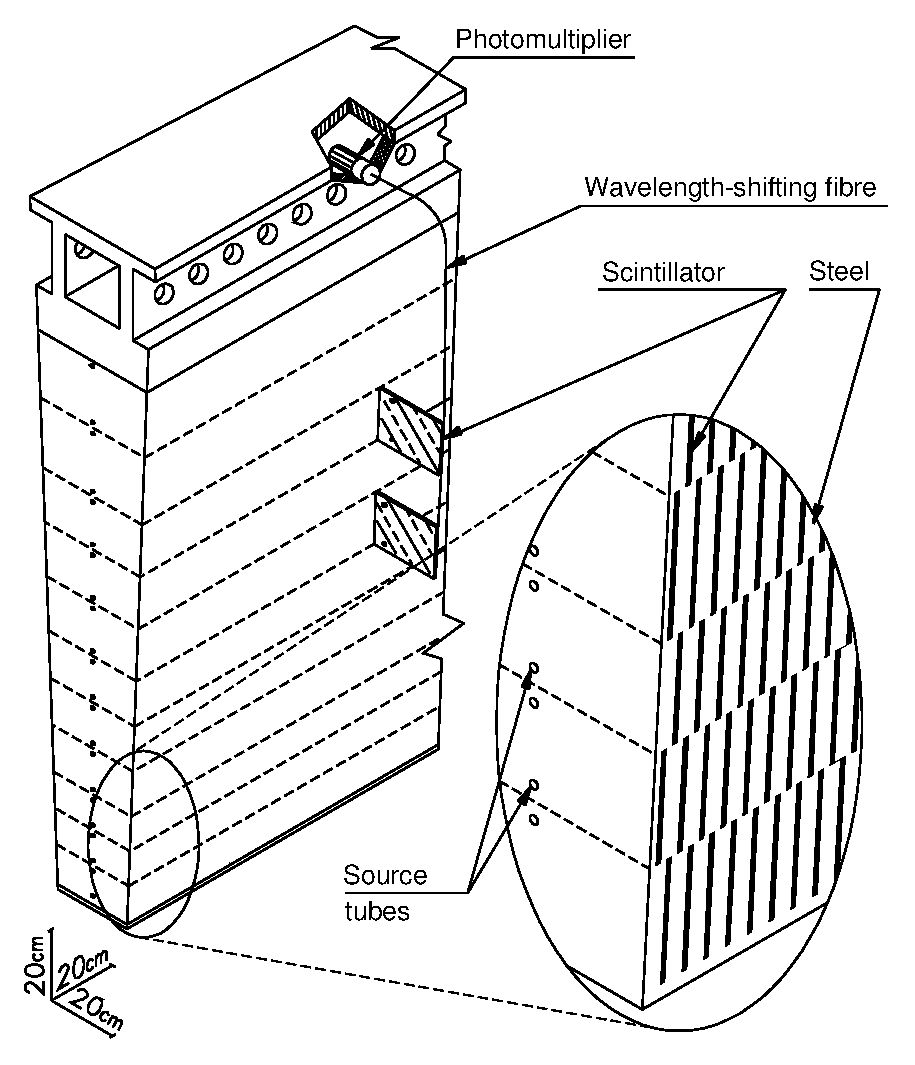
\includegraphics[width=0.5\linewidth,angle=0]{Detector/TileCal_Module3}
\end{center}
%\centerline{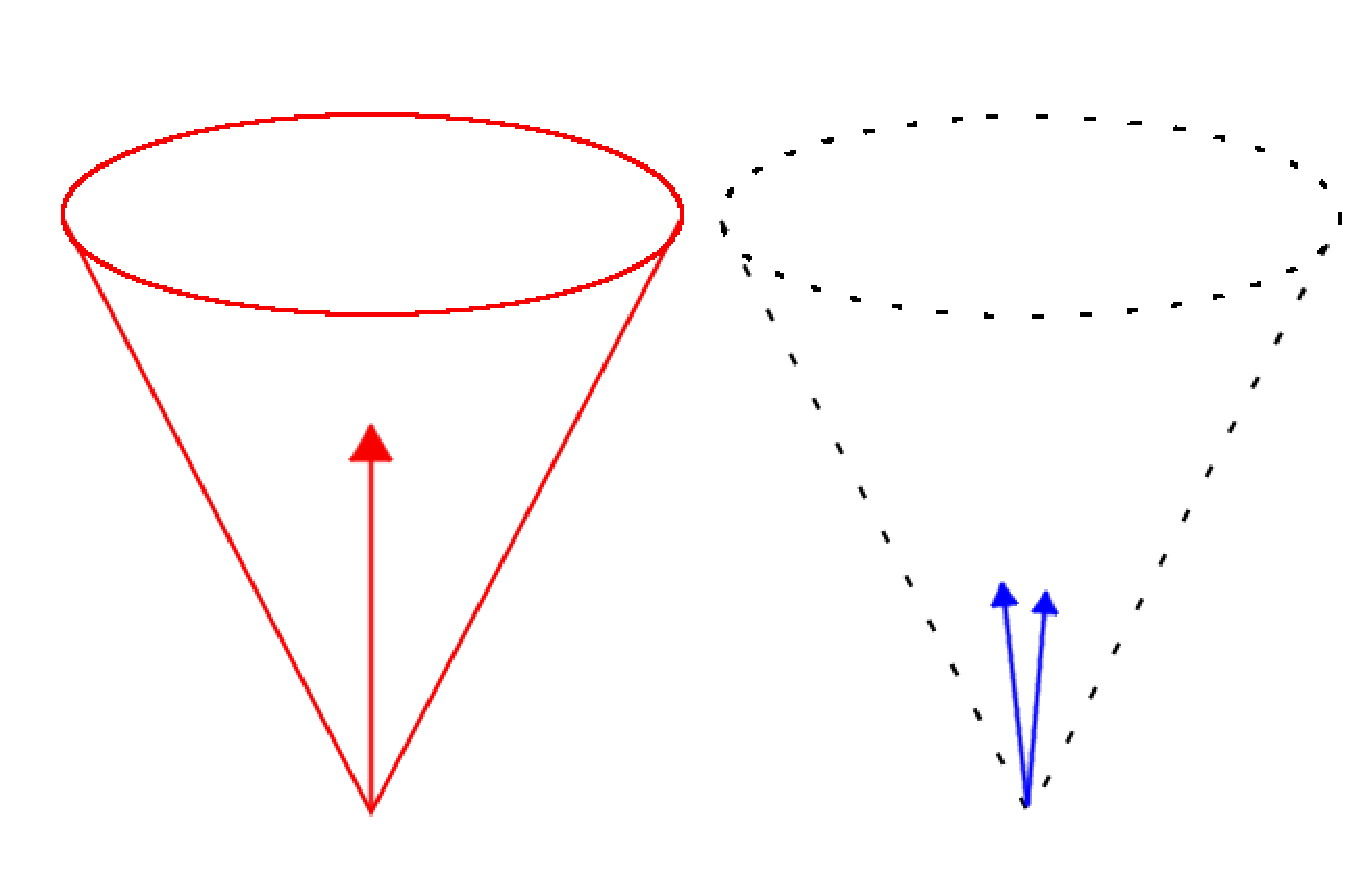
\epsfig{file=./figs/collinear.eps  , width=0.95\textwidth}}
\caption[Schematic of a tile calorimeter module]{Schematic of a tile calorimeter module. Alternating layers of master plates and spacer plates are glued together, with scintillating tiles positioned in the gaps in this structure.}
\label{fig_tile_module}
\end{figure}
The scintillating tiles are made of polystyrene, which produces scintillation light in the ultra-violet range when excited by the passage of showering particles. The polystyrene is doped with fluors that shift the wavelength of this light into the visible spectrum. Optical fibres are coupled to two sides of each scintillator tile, and are used to carry light from the tiles to the Photomultiplier tubes (PMTs), which are housed within the mechanical support structure of the calorimeter. The PMTs then convert the scintillation light to an electronic signal.


%central barrel (5.8 metres long) and two extended barrel regions that are located outside the end-caps
%
%has a depth of $\sim 7.4 \lambda$.
%
%
%
%tile steel/scintillator
%scintillators are polystyrene based, scintillation light is UV, but polystyrene doped with wavelength shifting fluors that move the wavelength into the visible spectrum.

\subsubsection{End-Cap Calorimeters}

The Electromagnetic End-Cap  (EMEC) and Hadronic End-Cap (HEC) Calorimeters are liquid argon calorimeters housed within the end-cap cryostats at either end of the detector.

The EMEC covers the pseudorapidity range $1.375 < |\eta| < 3.2$, and has a similar design to the EM Barrel calorimeter. As with the barrel, the absorber is formed from accordion shaped layers of lead sheets, while the active regions consist of the liquid argon gaps between these layers. Honeycomb spacers are used to keep the electrodes positioned in the centres of these gaps. A module of the EMEC is shown in Figure~\ref{fig_EMEC_module}.

The EMEC consists of two coaxial wheels, with the boundary between wheels located at $|\eta| = 2.5$, matching the acceptance of the ID. The inner wheel uses absorber sheets of thickness 2.2mm, giving the calorimeter a depth of $26 - 36 X_0$ in the region $2.5 < | \eta| < 3.2 $, while the absorber plates in the outer wheel are thinner (1.7mm) giving the calorimeter a depth of $24 -34 X_0$ in this region. Each wheel is subdivided into eight wedge-shaped modules. Due to the accordion shape of the absorber layers, there are no discontinuities in the calorimeter between adjacent modules. As with the EM barrel, the structure of the EMEC is completely symmetric with respect to azimuthal angle. The number of readout layers and their granularities are dependant on pseudorapidity; this information is summarised in Table~\ref{table_gran_emec}. 

\begin{figure}[tb]
\begin{center}
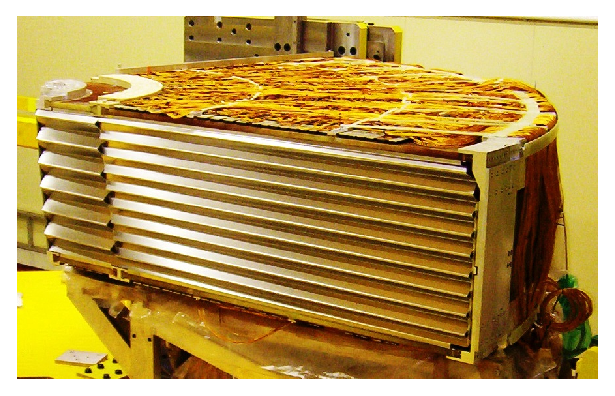
\includegraphics[width=0.8\linewidth,angle=0]{Detector/EMEC_module}
\end{center}
%\centerline{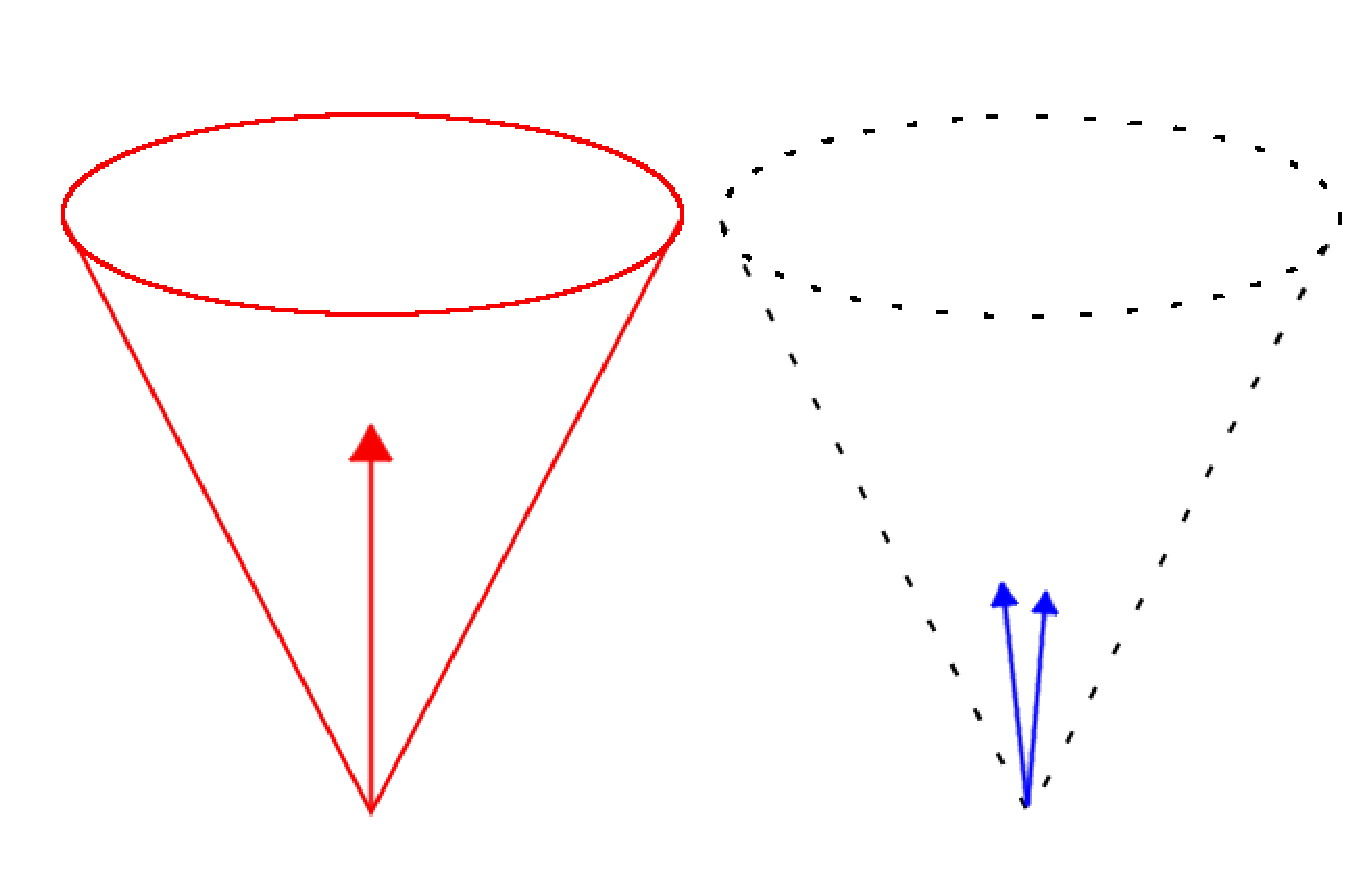
\epsfig{file=./figs/collinear.eps  , width=0.95\textwidth}}
\caption[Photograph of an EMEC module.]{photograph of an EMEC module, showing the accordion structure of the absorbers. The boundary between the inner wheel and the outer wheel can be seen towards the left, where the shape of the absorber plate changes.}
\label{fig_EMEC_module}
\end{figure}

\begin{table}[!htbp]
\begin{center}
\begin{tabular}{|l|l|l|l|}
\hline
pseudorapidity & layer 1 & layer 2& layer 3\\
\hline
$1.375 < |\eta| < 1.425$ &  $0.050 \times 0.1$ & $0.050 \times 0.025$ & \multirow{2}{*}{-} \\
\cline{1-3}
$1.425 < |\eta| < 1.5$ & $0.025 \times 0.1$    & \multirow{5}{*}{$0.025 \times 0.025$} & \\
\cline{1-2} \cline{4-4}
$1.5 < |\eta| < 1.8$ &   $0.0031 \times 0.1$   & &\multirow{4}{*}{$0.050 \times 0.025$} \\
\cline{1-2}
$1.8 < |\eta| < 2.0$ &  $0.0042 \times 0.1$    & & \\
\cline{1-2}
$2.0 < |\eta| < 2.4$ &  $0.0063 \times 0.1$    & &\\
\cline{1-2}
$2.4 < |\eta| < 2.5$ &  $0.025 \times 0.1$     & &\\
\hline
$2.5 < |\eta| < 3.2$ &  $0.1 \times 0.1$       & $0.1 \times 0.1$ & - \\
\hline
\end{tabular}
\end{center}
\caption[Readout granularity for the EMEC]{Readout granularity for the EMEC~\cite{detector_paper}, expressed as $\Delta \eta \times \Delta \phi$.}
\label{table_gran_emec}
\end{table}




% The inner wheel ($2.5 < | \eta | < 3.2$) consists of two layers, both of which have granularity $\Delta \eta \times \Delta \phi = 0.1 \times 0.1$. The inner part of the outer wheel ( $1.5 < |\eta| < 2.5$) consists of three layers, with the second layer having a granularity of $0.025 \times 0.025$ and the third having a granularity of $0.05 \times 0.025$. The granularity of the first layer increases from $\sim 0.003 \times 0.1$ at $|\eta| = 1.5$ to $0.025 \times 0.1$ at $|\eta| = 2.5$. 
%
%thickness of lead in inner and outer wheels.
%
%The readout of inner wheel has a granularity of $0.1 \times 0.1$ in $\Delta \eta \times \Delta \phi$. The granularity of the outer wheel varies with pseudorapidity, but is at its finest ($0.003 \times 0.1$) in the region $ 1.5 < | \eta | < 1.8$.
%\red{more detail about layers, granularity}







%HEC

%\red{why copper?}
The HEC calorimeters~\cite{HEC_construction} utilise a parallel plate geometry, which consists of alternating layers of copper and liquid argon oriented at right angles to the beam. Each side of the HEC consists of front wheel and a rear wheel, each of which is divided azimuthally into 32 wedge-shaped modules. The front wheel is comprised of a front plate which is 12.5 mm thick, as well as 24 copper plates, each of which is 25mm thick. The rear wheel contains a front plate that is 25mm thick, and is followed by 16 plates of thickness 50mm. 

In both wheels, the liquid argon gaps formed between the absorber plates have a depth of 8.5mm. These gaps are divided into four sub-gaps of thickness $\sim$2mm by a set of three parallel electrodes, forming an electrostatic transformer~\cite{1990NIMPA}. This makes it easier to match the impedance of the calorimeter channel to the readout electronics. The signal is read off a central pad in the middle electrode, with shapes etched into these pads determining the read-out structure. Cells in the HEC have a granularity of 0.1 $\times$ 0.1 in $\Delta\eta \times\Delta\phi$ for $|\eta| < 2.5$, and  0.2 $\times$ 0.2 at higher $|\eta|$.
%\red{why copper?}

\begin{figure}[tb]
\begin{center}
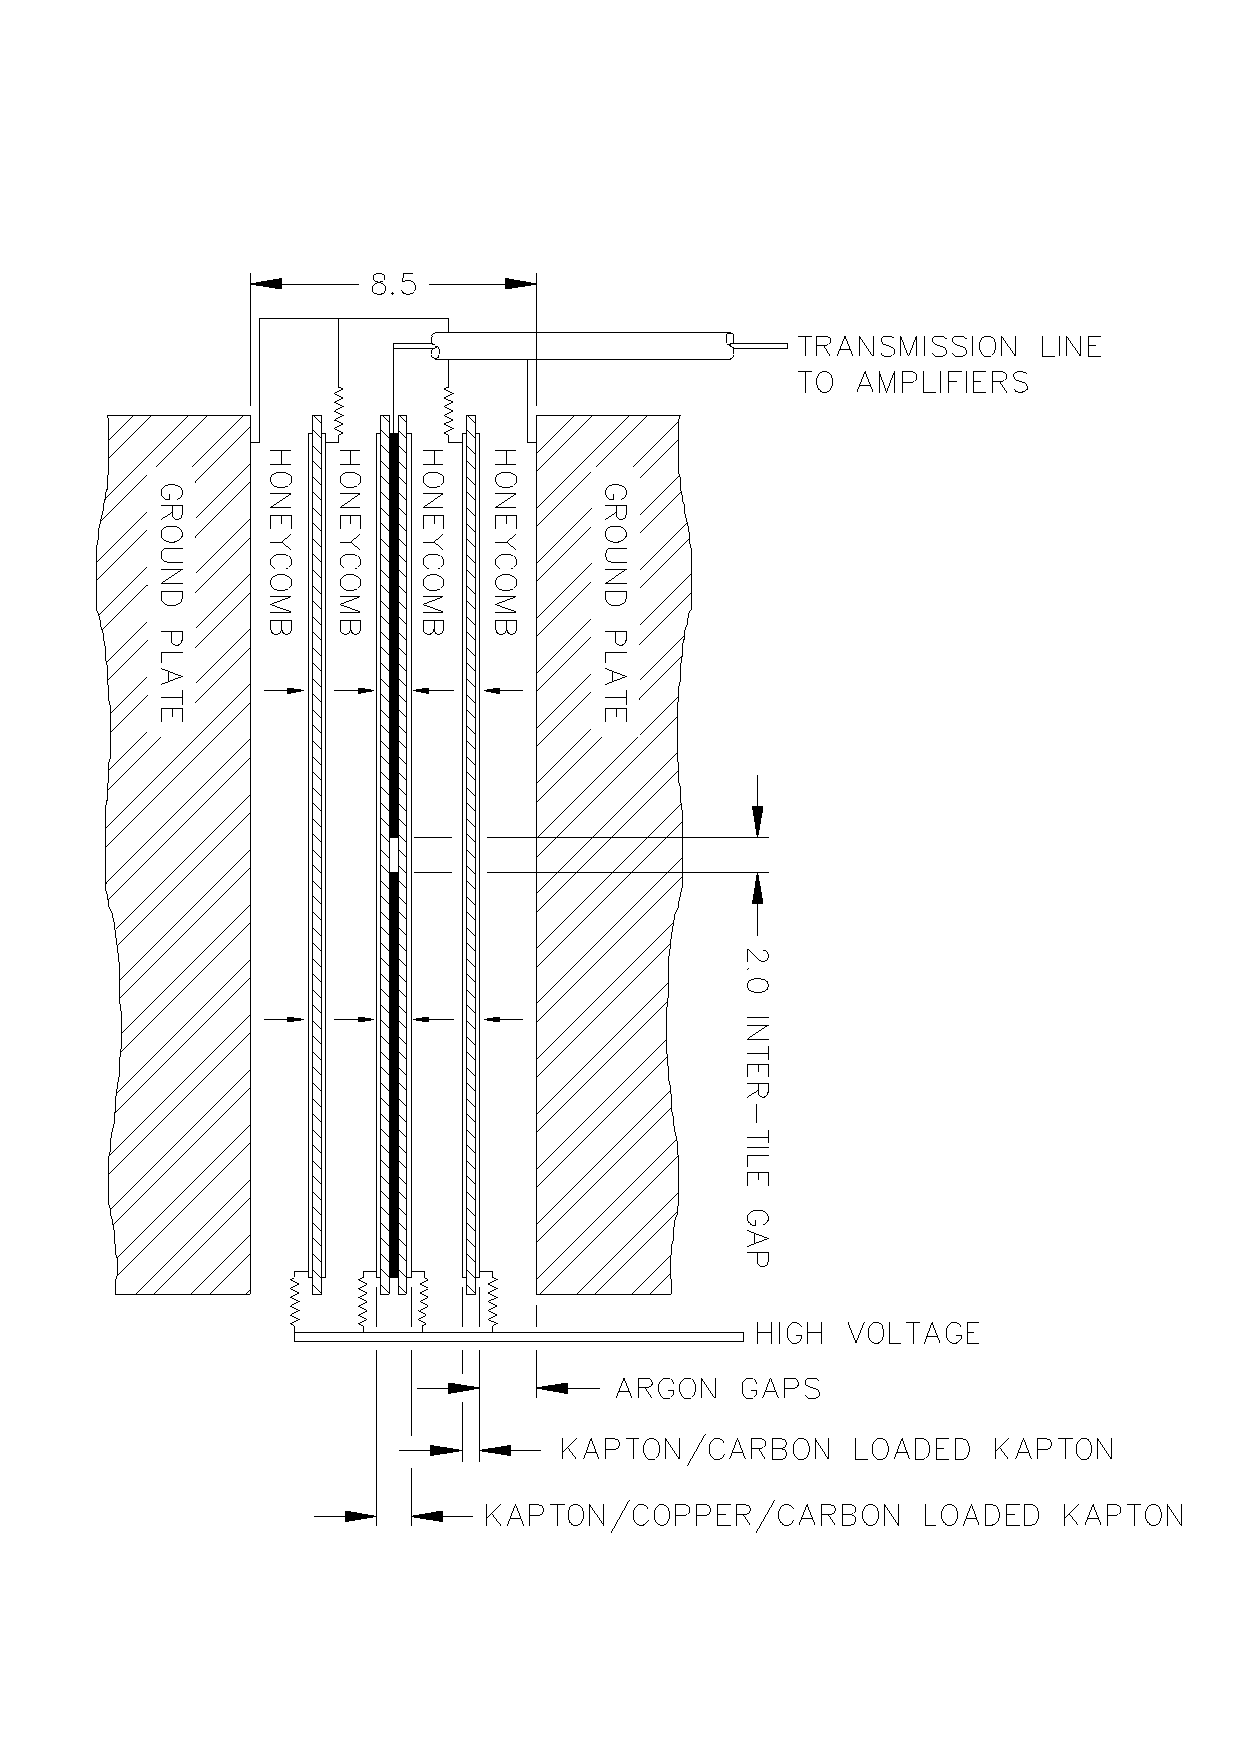
\includegraphics[width=0.5\linewidth,angle=0]{Detector/HEC_estM}
\end{center}
%\centerline{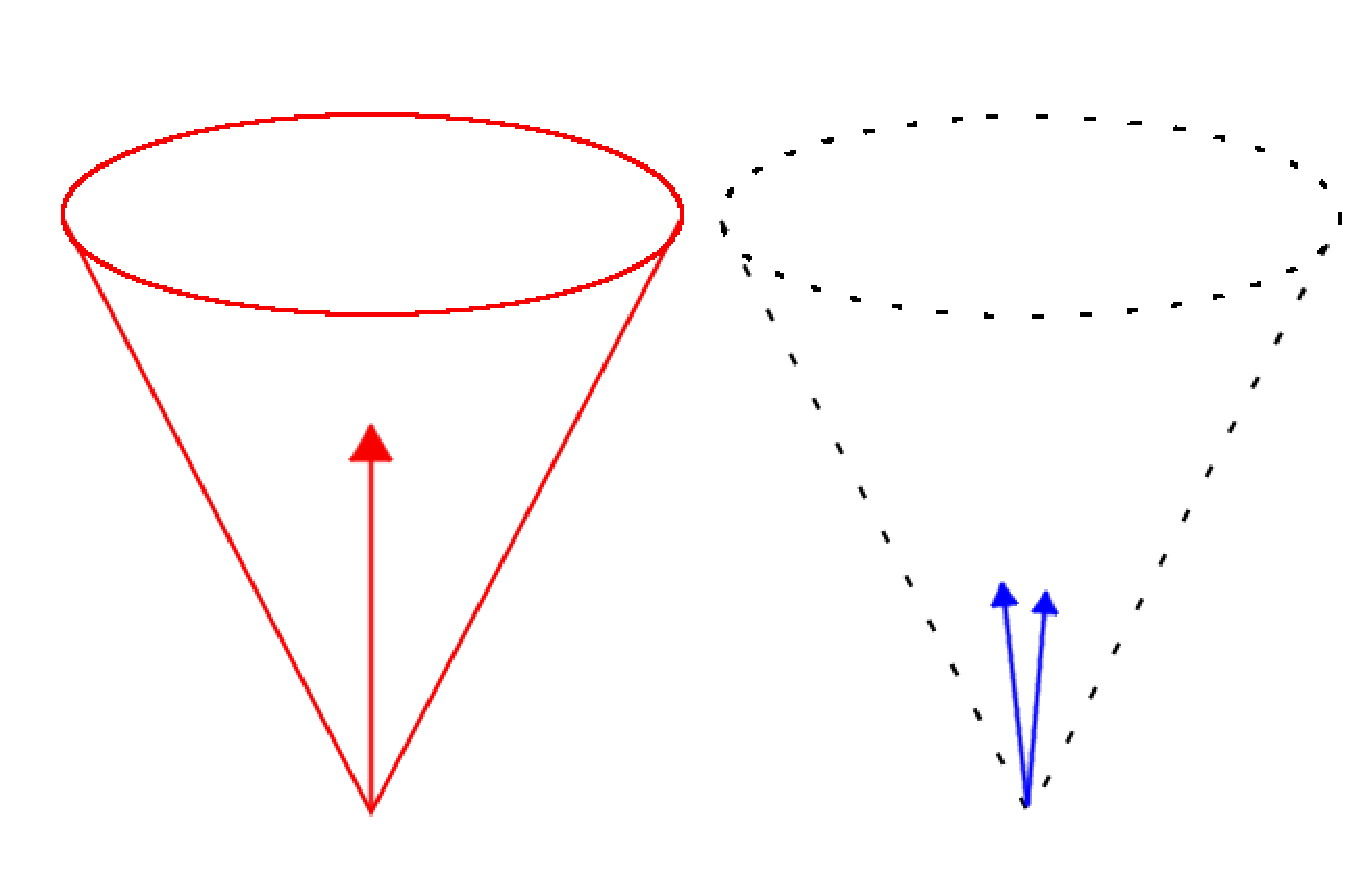
\epsfig{file=./figs/collinear.eps  , width=0.95\textwidth}}
\caption[Electrode structure in the HEC]{Electrode structure in the HEC. Electrodes are arranged to form an electrostatic transformer}
\label{hec_electrode_fig}
\end{figure}
%Central plate used to read out signal, readout structure is embedded/etched on this plate. granularities.
%
%
%Each gap is divided into 
%
% 
%HEC,  cu / LAr
%
%hec consists of two wheels, Hec 1 and Hec2, each wheel has two longitudinal sections
%
%made of alternating layers of Cu and LAr. Cu consists of flat plates normal to the beam.



%%Em barrel
%rapidity range (central barrel, extended barrel - tile)
%
%
%Tile
%
%End cap (EMEC/HEC)



%Tile
%
%LAR
%EM barrel
%EMEC
%HEC
%\clearpage
\subsection{Forward Calorimeters}
\label{chap_Detector_FCal}
%Be Consistent - specify cold dimensions

%figures to add:
%FCal in support tube
%electrode with tungsten slugs



The \atlas Forward Calorimeters (FCal) are located just outside the beampipe, with their front faces situated 4.7~m on either side of the \atlas interaction point. These are liquid argon based calorimeters, and are located within a support tube inside the end-cap cryostat (Figure~\ref{fig_cut}). They cover the pseudorapidity region $3.1 < |\eta| < 4.9$.

\begin{figure}[tb]
\begin{center}
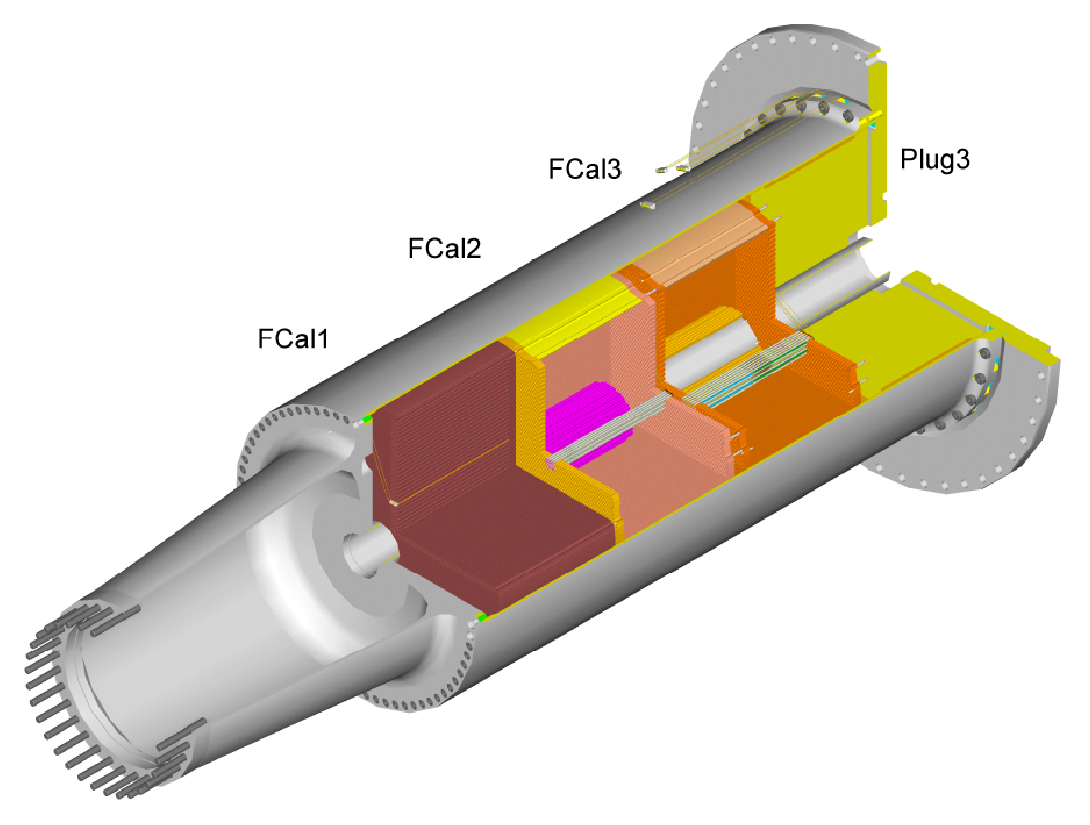
\includegraphics[width=0.8\linewidth,angle=0]{TBoverview/FCal_support_cutaway.eps}
\end{center}
%\centerline{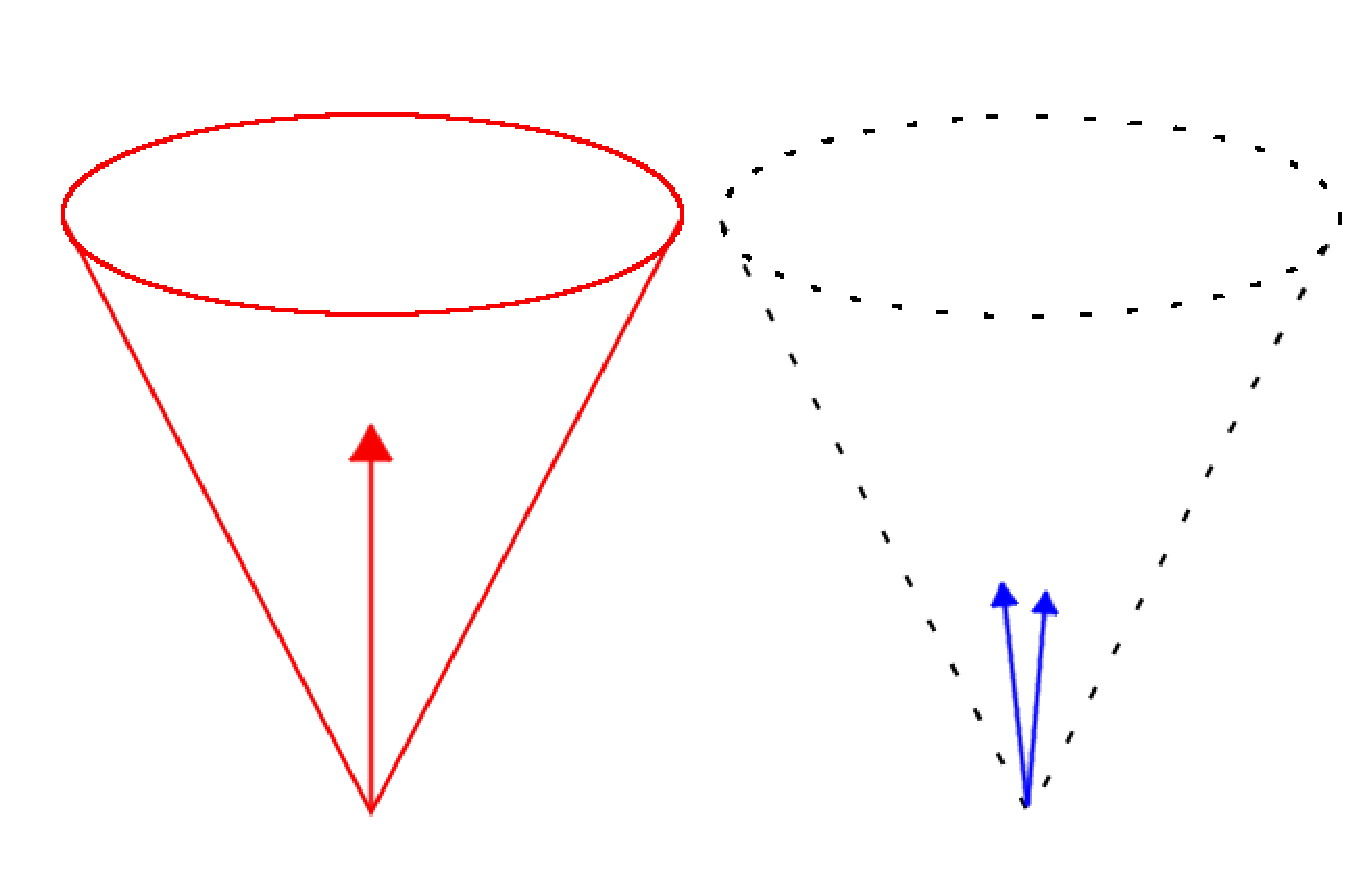
\epsfig{file=./figs/collinear.eps  , width=0.95\textwidth}}
\caption[Cut-away view showing the FCal within its support tube]{Cut-away view showing the FCal within its support tube\cite{FCal_jinst_2010}. The region inside the support tube and just upstream of the calorimeter is evacuated in ATLAS.}
\label{fig_cut}
\end{figure}


Each FCal consists of three modules, one electromagnetic module (FCal1) and two hadronic modules (FCal2 and FCal3). Each module has a cylindrical shape, with an outer radius of 449~mm and a depth of 444~mm. A plug made of a brass alloy has a similar shape and is located behind the hadronic modules in order to provide additional shielding for the muon chambers behind it. As the FCal operates at a temperature just below 90K in \atlas, ``cold'' values will be used in the following when quoting dimensions, densities, or other temperature-dependent quantities. %\red{ radiation and interaction lengths}.

The electromagnetic modules of the FCal were produced by the University of Arizona. Each module consists of a stack of circular copper plates with an inner radius of 72 mm and an outer radius of 449~mm.\cmt{On the ``A'' side, the FCal 1 module consists of 18 plates of thickness 24 mm, whereas on the ``C'' side 19 slightly thinner plates are used.}  Each plate is drilled with a hexagonal array of holes into which the electrodes were inserted. This was done in a way that established a good electrical connection between the outside of the electrode and one of the copper end-plates. Each electrode consists of a copper tube (the cathode) containing a copper rod (anode) around which a radiation-hard PEEK fibre is wrapped. The inner radius of the copper tubes is 2.62~mm while the radius of the copper rods is 2.35mm, thus leaving a gap of 267~$\mu$m which is filled with liquid argon. The PEEK fibre has a diameter of 250~$\mu$m, and is present to keep the rod positioned in the centre of the tube, thus maintaining the uniformity of the LAr gap throughout the electrode and keeping the rod electrically isolated from the tube. Typical gap sizes used in traditional LAr calorimeters are on the order of a few millimetres, as is the case for the EM Barrel, EMEC and HEC calorimeters. However, as the FCal is located at high pseudorapidity, minimum bias events will deposit energy in it at a very high rate. The smaller gap size is required in order to reduce the drift time across the gap, and thus preventing the high rate of ionisation from causing a build-up of positive ions in the liquid argon. Positive ion buildup can distort the electric field in the LAr gap, thus distorting the signal from the electrode.
The distance between electrodes in FCal1 is similar to the \moliere radius  for copper. EM showers in the FCal should thus spread across several electrodes, allowing the calorimeter to sample the shower effectively. Copper also allows the FCal1 module to conduct heat efficiently. The cryostat temperature is kept at about 88.5K, while the boiling point for liquid argon within the cryostat is 92.7K. With the LHC running at design luminosity, minimum bias events are expected to heat the FCal at a rate of about 45W, with about half of that power going into FCal1. A finite element analysis estimated that this heating would cause a temperature increase within the FCal of no more that 1.5K, which is not enough to cause the liquid argon to boil\cite{FCal_jinst_2010}.

% This is important, as it prevents the energy deposited within the FCal from raising the %temperature of the liquid argon above its boiling point. 
%
%
%%maintained below 90K
%%boils at 92,7K
%
%
%%drift time of 61ns in FCal1, compared to 450 ns for a 2mm gap
%%energy density lower in hadronic modules, so can have a larger gap
%FCal1 28X0 deep, 2.7 lambda
%FCal2 and 3 are 3.6 and 3.7
%
% build up from occurring in the LAr due to  the high rate of ionisation. Moliere radius similar size to electrode spacing

The hadronic modules of the FCal were produced at the University of Toronto (FCal2) and at Carleton University in Ottawa (FCal3). They have a similar design to the electromagnetic module, however tungsten is used as the absorber material instead of copper. Each of the hadronic modules uses two copper end plates drilled with a hexagonal array of holes, each of which holds an electrode. The electrodes use copper tubes for their cathodes and rods made of pure tungsten (with density 19.2 $\mathrm{g}/\mathrm{cm}^3$) for the anodes. The absorber matrix is formed from small slugs of tungsten alloy (``WFeNi'' - 97\% Tungsten/2\% Iron/1\% Nickel) positioned in the gaps between the electrode tubes, as shown in Figure~\ref{slugfig}. The material composition and density of the calorimeter components are important factors when establishing a description of the calorimeter to be used by simulations. By themselves, the WFeNi slugs have a measured mean density of 18.3~$\mathrm{g}/\mathrm{cm}^3$. When considering the WFeNi slugs, the copper electrode tubes, and any spaces in the absorber matrix that are filled with liquid argon, the average density of absorbing material (excluding electrode rods) in the hadronic modules is estimated to be 14.33 $\mathrm{g}/\mathrm{cm}^3$ for FCal2 and 14.45 $\mathrm{g}/\mathrm{cm}^3$ for FCal3~\cite{Archambault:2009zza}. 
%A diagram showing the way in which the WFeNi slugs are positioned amongst the electrodes is shown in figure~\ref{slugfig}

\begin{figure}[tb]
\begin{center}
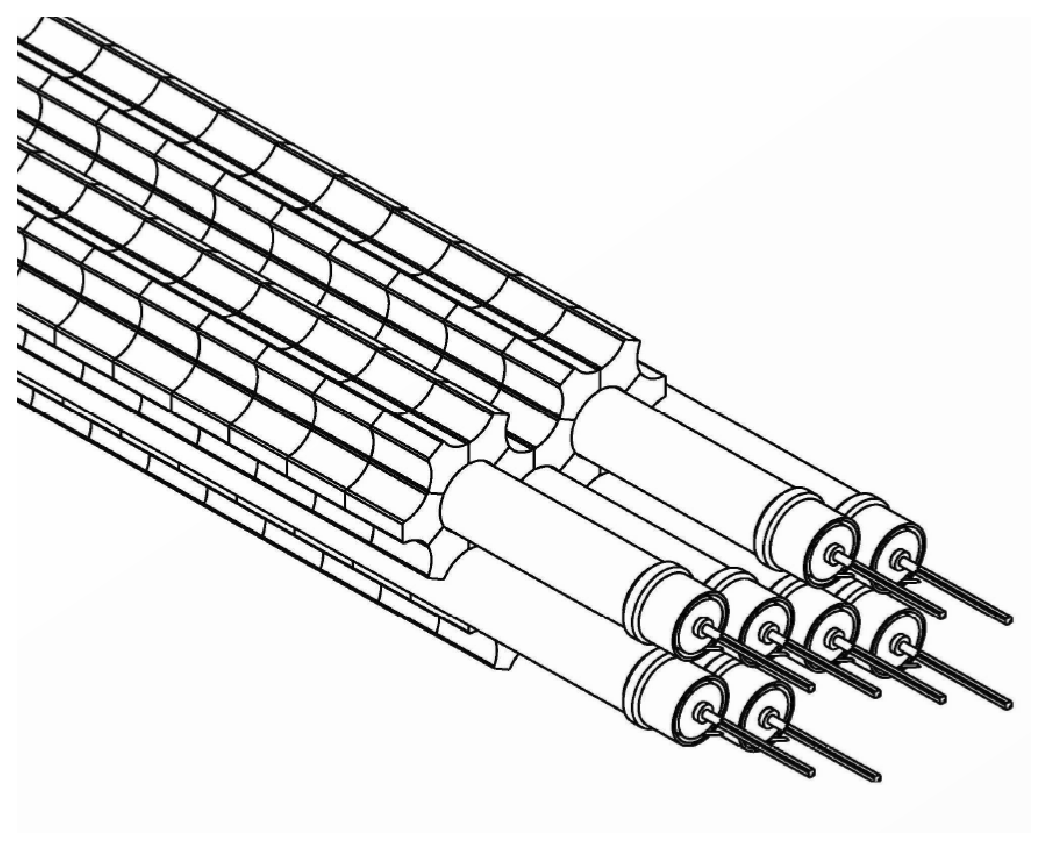
\includegraphics[width=0.5\linewidth,angle=0]{TBoverview/rods_slugs}
\end{center}
%\centerline{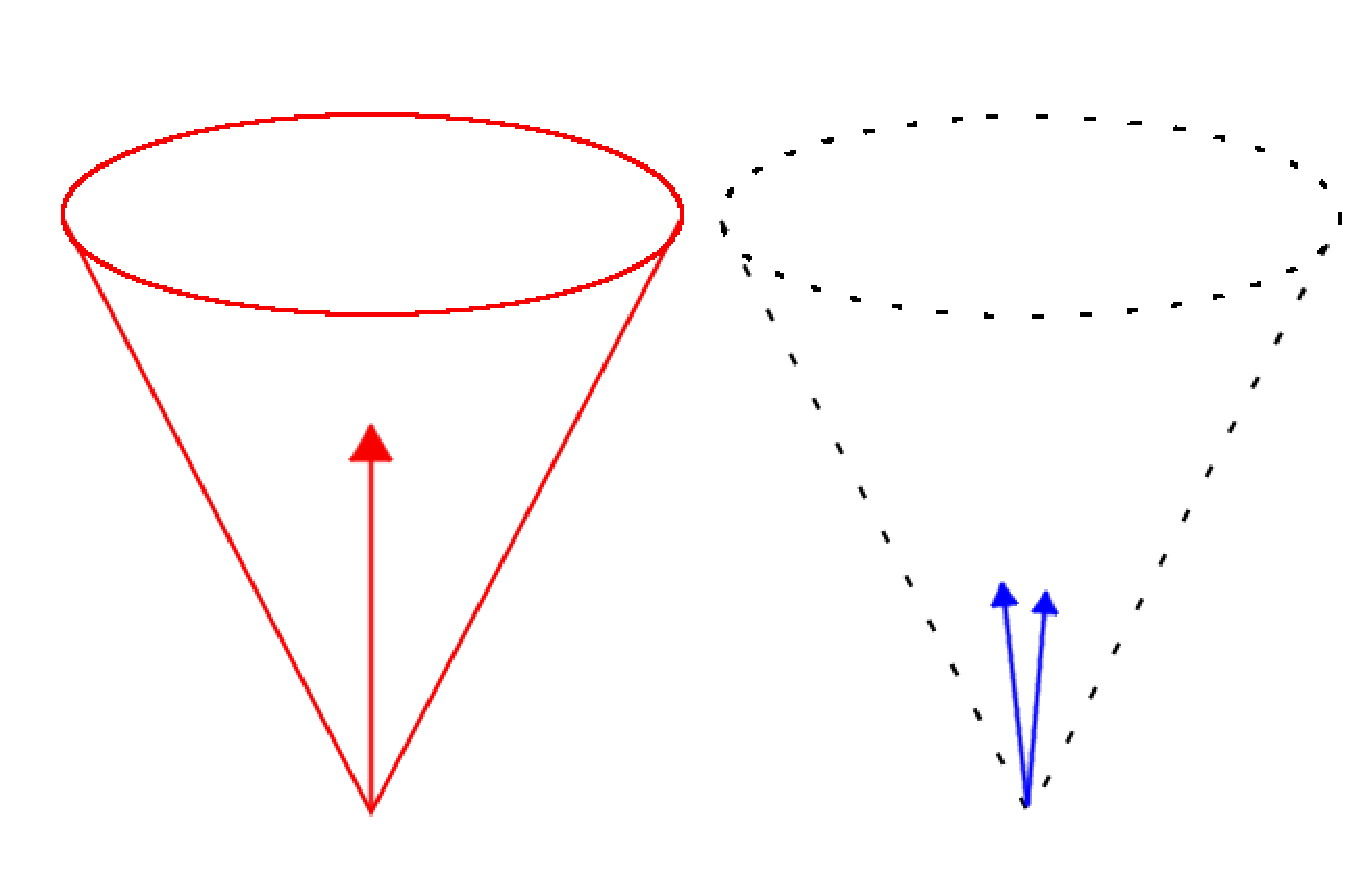
\epsfig{file=./figs/collinear.eps  , width=0.95\textwidth}}
\caption[Electrode/slug arrangement in the FCal.]{Diagram showing the arrangement of electrodes and slugs in the hadronic modules~\cite{FCal_jinst_2010}.}
\label{slugfig}
\end{figure}



%As charge is deposited in the liquid argon, it drifts due to the electric field present in the electrode, causing a current which is used as a signal. The electronics chain used to read out and process this signal is discussed in detail in section~\ref{sec_FCal_electronics}.




%pic of FCal 1/Moliere radius
%pic of FCal in support tube
%pic of FCal2/3 matrix with electrode


%little bit about electronics, which bits are summed, etc.
%dimensions, some photos.
%
%
%table
%module, material, electrode separation, no electrodes, rod diameter, tube inner diameter, lar gap, average absorber density


%rotate the table
%
%\begin{table}[h!bp]
%\begin{center}
%\begin{tabular}{|l|l|l|l|l|l|l|l|}
%\hline
%module & absorber material & module inner diameter & electrode separation & rod diameter & tube  inner diameter & LAr Gap & distance from IP \\
%% module inner radius
%\hline
%\hline
%FCal1 (EM) & Copper & 720 $mm$ & 7.5 $mm$ & 2.35 $mm$ & 2.62 $mm$ & 267 $\mu m$ & 4668.5 $mm$ \\
%\hline
%FCal2 (Had) & Tungsten & 790 $mm$ & 8.2 $mm$ & 2.47 $mm$ & 2.84 $mm$ & 375 $\mu m$ & 5128.3 $mm$\\
%\hline
%FCal3 (Had) & Tungsten & 860 $mm$ & 9.0 $mm$ & 2.75 $mm$ & 3.25 $mm$ & 500 $\mu m$ &  5602.8 $mm$\\
%\hline
%\end{tabular}
%\end{center}
%\caption{Dimensions of the FCal modules.}
%\end{table}
%
%
%
\begin{table}[tb]
\begin{center}
\begin{tabular}{|l|l|l|l||}
\hline
Quantity & FCal1 & FCal2 & FCal3 \\
\hline
\hline
Absorber material & Copper & Tungsten & Tungsten\\
\hline
Module inner diameter & 72 mm & 79 mm & 86 mm\\
\hline
Electrode Separation & 7.5mm & 8.62 mm &9.0mm \\
\hline
Rod Diameter & 2.35 mm & 2.47 mm & 2.75 mm\\
\hline
Tube inner diameter & 2.62 mm & 2.84 mm & 3.25 mm \\
\hline 
LAr Gap & 267 $\mu$m & 375 $\mu$m & 500 $\mu$m \\
\hline
Distance from IP to front face & 4668.5mm & 5128.3 mm & 5602.8 \\
\hline
Number of electrodes & $\sim$ 12,000 & $\sim$ 10,000 & $\sim$ 8000 \\
\hline
\end{tabular}
\end{center}
\caption{Dimensions of the FCal modules.}
\end{table}

\subsubsection{FCal Electronics}
\label{sec_FCal_electronics}
%maybe move this to the detector chapter

%
%An electric field of \~ 1KV/mm is desired for liquid argon calorimeters. In The FCal, the rods in each electrode are connected to a high voltage supply while the electrode tubes are grounded. 
%
%In FCal1, Electrodes are ganged together in groups of four. The four rods are connected to an interconnect board which is supplied by a single HV line \red{(coax?)}. 

%The high voltage is supplied to the electrodes through interconnect boards. In FCal1, electrodes are ganged together in groups of four to form a "tube group". The rods from these electrodes are connected to the interconnect board, which is supplied with HV via a coaxial cable. The cable supplying the HV is also used to read out the signal from the calorimeter, and so the signal (a current pulse) from the electrodes are summed together at the interconnect board.


An electric field of  $\sim$1KV/mm is conventional for liquid argon calorimeters. In order to provide this the rods of each electrode are supplied with high voltage while the tubes are grounded. Showering particles ionise the liquid argon, leaving free electrons and $\mathrm{Ar}^+$ ions in the gap. The electric field in the gap then causes this charge to drift resulting in a current pulse. This pulse is triangular in shape, having a fast rise time ($\sim$1 ns) and taking $\sim$61 ns (in FCal1) to return to zero~\cite{FCal_jinst_2010}. The height of the pulse peak depends on the amount of charge deposited in the liquid argon, and is thus proportional to the amount of energy deposited in the liquid argon \footnote{The energy required to ionise an atom of argon is 15.8 eV.}.
 
% Charge is deposited \cmt{liberated?} in the gap as showering particles ionise the liquid argon.
%Showering particles ionise the liquid argon, leaving free electrons and $\mathrm{Ar}^+$ ions in the gap.

 

%In FCal1, electrodes are ganged together in groups of four to form a "tube group". 

\begin{figure}[tb]
\begin{center}
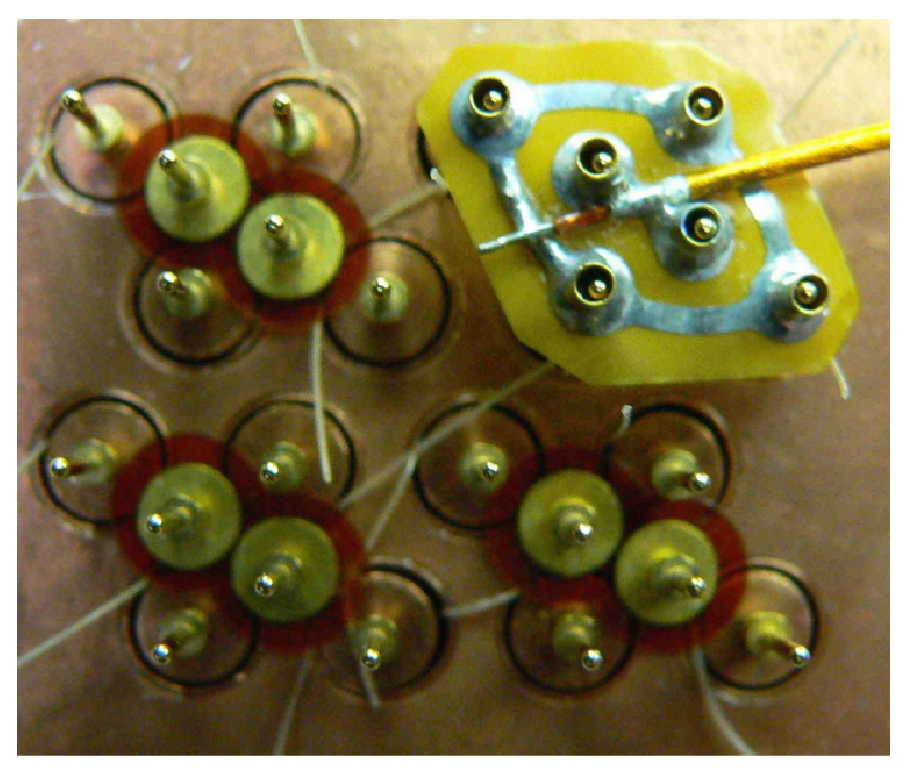
\includegraphics[width=0.6\linewidth,angle=0]{TBoverview/ICB.eps}
\end{center}
%\centerline{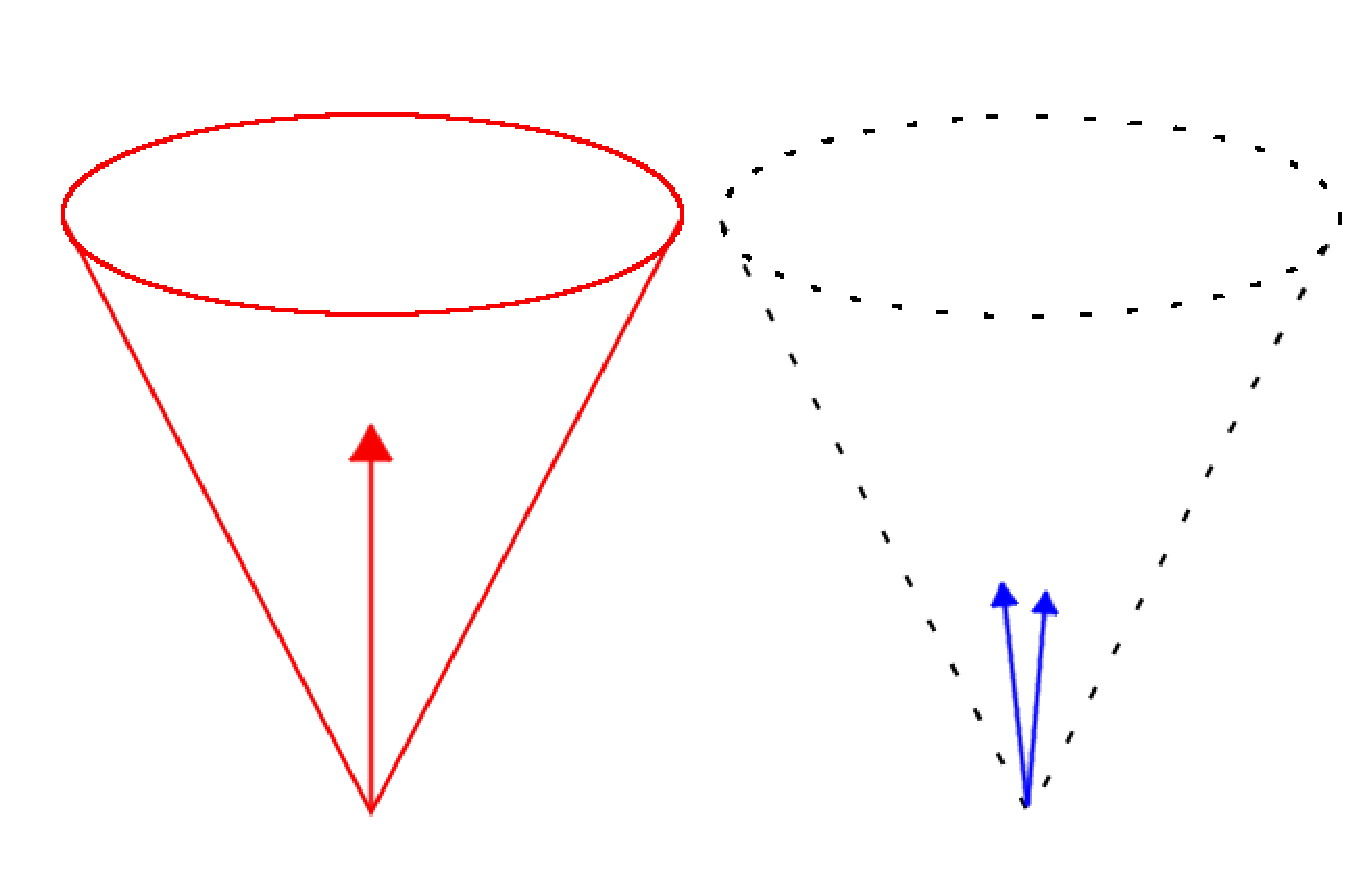
\epsfig{file=./figs/collinear.eps  , width=0.95\textwidth}}
\caption[Photograph of an FCal endplate]{Photo of an endplate of FCal1, taken during assembly, showing the interconnect board and the coaxial cable used for HV delivery and readout~\cite{FCal_jinst_2010}. Also visible are the PEEK fibres used to keep the rods centred within the tubes. The two central pins in each group are used to ground the end plate, and thus the tubes, while the four exterior pins provide HV to the rods and carry the signal off the electrode.}
\label{interconnect_fig}
\end{figure}

The signal is read out via a coaxial cable that also supplies the electrodes with high voltage. Electrodes in the FCal are ganged together on interconnect boards to form ``tube groups''. Tube groups are formed from four electrodes in FCal1, six electrodes in FCal2, and nine electrodes in FCal3. Gold-plated signal pins connect the rods from these electrodes to the interconnect board, which is supplied with HV via a coaxial cable as shown in Figure~\ref{interconnect_fig}. The tubes are also grounded through this coax: each interconnect board is connected (via grounding pins) to the FCal end plate. \cmt{The line supplying HV to the tube group also serves as a readout line, carrying the signal off the interconnect board.}As the interconnect board connects electrodes in parallel, the signal carried off the interconnect board is the sum of the current pulses in each electrode of that tube group.

%As the HV line supplying a tube group is also used to read out the signal, the current pulses from each electrode are summed together on the interconnect board to form one signal for the entire tube group. 

%
%
%
%HV line is also read out line
%
%signal is read off the interconnect board
%
%pulses in all tubes summed on the interconnect board.
%
%
%
%signal read off the interconnect board is the sum of the current pulses in each electrode.

%\blue{Impedance matching (lack of) between electrodes and cable}
 \begin{figure}[tb]
\begin{center}
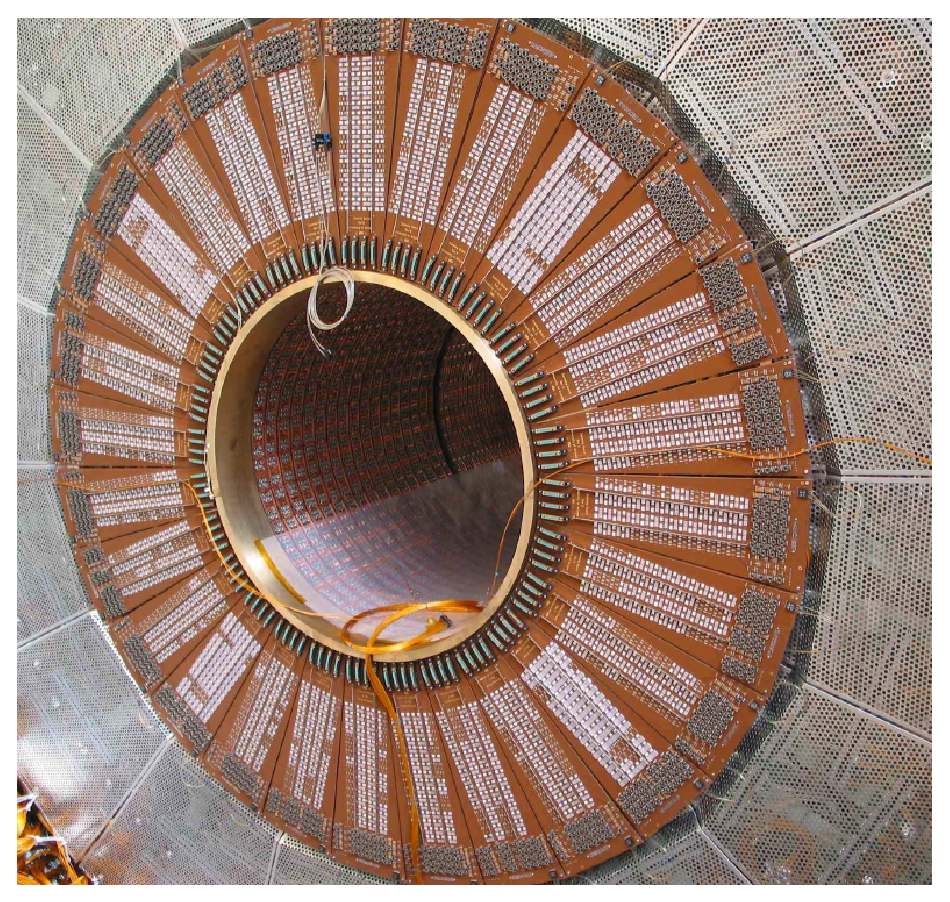
\includegraphics[width=0.8\linewidth,angle=0]{TBoverview/summingboards.eps}
\end{center}
\caption[Summing boards for the FCal.]{The FCal summing boards mounted on the rear of the HEC\cite{FCal_jinst_2010}}
\label{fig_summing_board_hec}
\end{figure}
%In \atlas, the signal from is read out from the end plate closest to the interaction point, whereas signals from FCal2 and FCal3 are read out from the end plate furthest from the interaction point. The shower maximum tends to be located between FCal1 and FCal2, and so the readouts are arranged in this way to minimise exposure of the electronics to radiation. 
\begin{figure}[tb]
\begin{center}
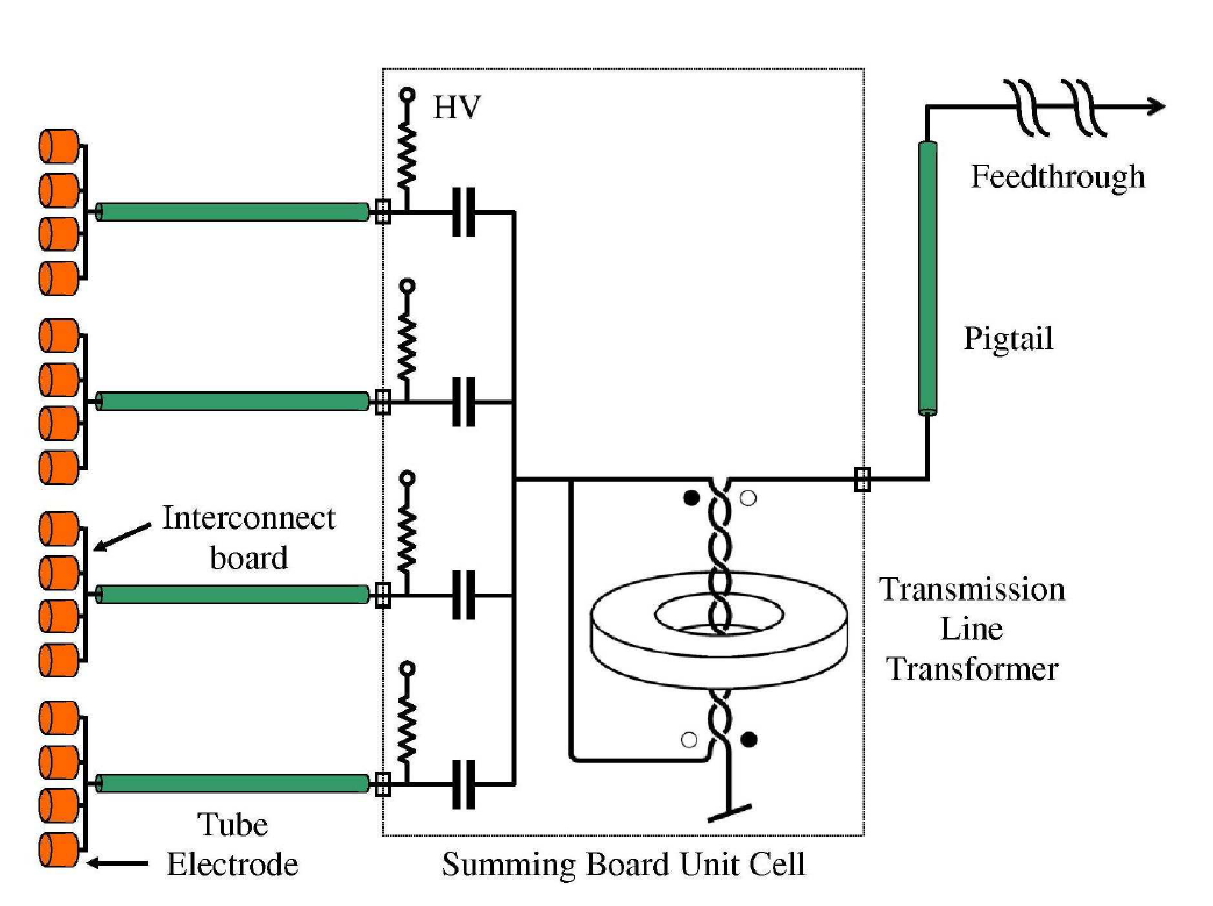
\includegraphics[width=0.8\linewidth,angle=0]{TBoverview/summing_board.eps}
\end{center}
\caption[Readout chain for a single summed FCal channel.]{Diagram of the FCal readout chain for a single summed channel. Summed channels are composed of four tube groups, which each consist of 4/6/9 electrodes in FCal1/FCal2/FCal3.}
\label{fig_sum_board}
\end{figure}

The readout lines are then fed out to summing boards, which are located on the rear of the HEC (i.e. inside the end-cap cryostats) as shown in Figure~\ref{fig_summing_board_hec}. On each summing board, signals from four interconnect boards are further combined to form a single readout channel. A typical FCal channel thus corresponds to four tube groups, which is equivalent to 16/24/36 electrodes in FCal1/FCal2/FCal3. The summing is carried out through a transmission line transformer, which serves to match the impedance of the readout coax to that of the ``pigtail'' cable used to carry the signal away from the summing board (Figure~\ref{fig_sum_board}). A different HV source is used to supply each tube group in a given channel, so that if one source fails then the other three tube groups in the channel should still be powered. This has occurred in \atlas: one of the lines supplying HV to the A-side FCal was severed during installation. This line supplies HV to one quadrant of FCal3, leaving one quarter of the tube groups in the affected area without HV. The remaining tube groups still contribute signal to the channels in this area, and so the effect of the severed HV line is corrected for during reconstruction.

Near the inner and outer edges of the FCal the tube groups are irregularly shaped. It is not practical to sum these channels in a coherent manner, and these ``unsummed'' channels also provide better readout granularity at high $|\eta|$.  
%The unsummed channels located near the inner edge (high $\eta$) also provide a readout with finer $\eta-\phi$ granularity than summed channels would in this region.

%\red{febs used by all LAr electronics?}

``Pigtail'' cables are  used to carry the signal from the summing boards to the cryostat feedthrough. Outside the cryostat, a stripline cable is used to carry the signal from the feedthrough to the Front End Boards.

\subsubsection{Front End Boards}
\label{sec_FEB}
Front End Boards (FEBs)\cite{ATLAS_FEB_design} are used in the electronics chains of all liquid argon calorimeters. Much of the following discussion applies to the electronics associated with all of these calorimeters, however some of the details mentioned here are specific to the electronics chain of the FCal. \cmt{The FEBs used during the beam test were prototypes, and had a similar design to those currently being used in \atlas. }

On the FEB, the signal is amplified and then shaped. The shaping consists of one differentiation and two integration steps (CR-${\rm RC}^2$) resulting in a bipolar pulse shape. This is done in order to optimise the signal with respect to pileup and electronics noise\cite{TDR_LAR,ATLAS_FEB_design}. In the other LAr calorimeters it takes much longer for the triangular current pulse to drop from its peak value back to zero due to the larger gap size\footnote{This time is $\sim$400~ns in the EM barrel but only $\sim 60$ ns in FCal1~\cite{FCal_jinst_2010}}. In these cases the shaping also allows the signal to be read out much faster, as the relevant information can be obtained from the first $\sim 125$ ns of the shaped pulse. 
%shaped pulse can be read out in , can be read out much faster allows the EM barrel calorimeter it takes $\sim 400$ns for the current pulse to drop from its peak value back to zero. In this case, the shaping allows for the  \blue{and also to reduce the signal collection time. In the EM barrel, triangular pulse takes ~400ns to drop to zero. Charge present in the LAr is proportional to the height of this pulse, and so it is unnecessary to measure the entire pulse to obtain this information. Shaped pulse can be read out in ~100ns }. 
Three different gains (low, medium, and high) are used when amplifying the signal. The amplification used for high gain is about 10 times as much as that used for medium gain, which in turn is about 10 times higher than that used for low gain. Each shaping chip processes the signals from four channels. An additional output on this chip sums the four inputs and then shapes the result. This output is used in the formation of trigger towers, which are discussed in section~\ref{sec_triggers}.

Timing on the FEB is managed by a Trigger Timing Control (TTC) chip, which distributes clock pulses every  25ns. The signal (at each gain) is sampled at every 25ns, and stored (as an analog voltage) on a Switched Capacitor Array (SCA) circuit. The pulse shapes for the three FCal modules are illustrated in Figure~\ref{fig_pulsehape}, showing the times at which the signals are sampled. Each pulse consists of an initial positive lobe followed by a longer negative lobe, the start of which can be seen in the Figure. \cmt{Note that the first sample is taken before the pulse starts to rise}

\begin{figure}[tb]
\begin{center}
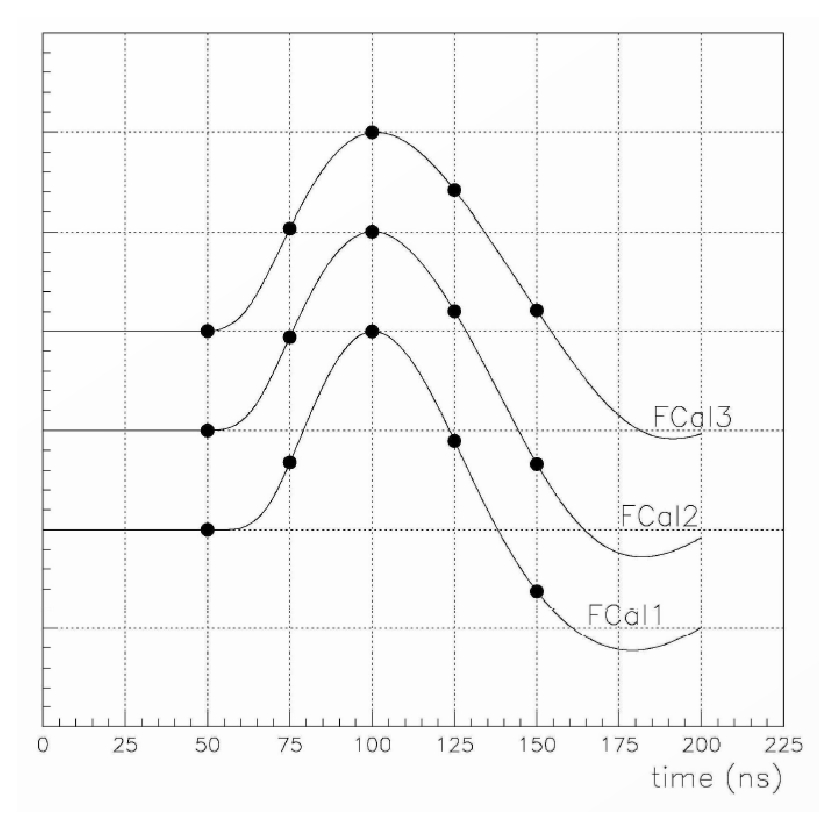
\includegraphics[width=0.6\linewidth,angle=0]{TBoverview/pulse_shapes.eps}
\end{center}
\caption[Pulse shapes for the FCal modules.]{Pulse shapes for each module. The dots indicate the times at which they are sampled and digitised.}
\label{fig_pulsehape}
\end{figure}

When a trigger signal indicates that an event should be read out, the pulse samples are read off the SCA and fed to an ADC (Analog to Digital Converter). For each sample the ADC then outputs a 12-bit signal\cmt{, which is a discretised voltage capable of taking one of 4,096 distinct levels}. Under normal operation only a single gain is read out of the SCA and digitised; a gain selector chip is used to determine which gain will yield the largest pulse height without saturating the ADC output. This is done by digitising a sample near the peak of the pulse at medium gain, and comparing the result to two pre-defined thresholds. If the value of the digitised sample lies between the thresholds then medium gain is used for the digitisation, otherwise low gain is used if the sample exceeds the upper threshold or high gain is used if the sample is smaller than the lower threshold.
%As the pulse shape has a negative lobe, a ``pedestal'' value must be subtracted from the digitised output in order to represent a negative value. 
In order to allow for negative values, e.g. samples taken on the negative lobe of the pulse, a ``pedestal'' value is subtracted from the digitised output. An offset voltage is added to the samples read from the SCA just prior to their digitisation~\cite{ATLAS_FEB_design}. This offset voltage is chosen such that the pedestal value is around 1,000 ADC counts, leaving around 3,000 ADC counts to represent the positive lobe of the pulse. For example, the negative lobe of a pulse may be sampled, and stored as a negative voltage in the SCA. Prior to digitisation, the sample is read from the SCA, and the offset voltage is added, such that the voltage to be digitised is positive. The digitised sample will then have a value of less than 1,000 ADC counts. When used to compute the channel energy (as discussed below), the pedestal value ($\sim$1,000 ADC counts) is first subtracted, such that the value associated with this sample is negative.

For the testbeam studies discussed in chapter~\ref{chapTB} the pedestal values were obtained from physics data on a run by run basis. For each channel, the first sample of each pulse was averaged over the entire run, and this value was used as the pedestal during reconstruction. Note that the first sample is taken before the pulse starts to rise, as illustrated in figure~\ref{fig_pulsehape}. In \atlas, the pedestal values for each channel are obtained from electronic calibration runs.


%The pedestal value During data taking the pedestal value was estimated \red{data taking pedestal monitored, reconstruction used average of first sample over a run.} 

%After shaping, the pulse has a bipolar shape. in order to obtain a pulse like that shown in figure~\ref{}.
%
%Febs used were prototypes, similar to final \atlas design
%trigger timing control TTC on FEB controls when data sampled/read out (every 25 ns)
%beam triggers not synched to this (unlike LHC)
%signal 

%The pulse is bipolar, prevents electronics being charged (?). Sampled at 25ns intervals, digitised. Pedestals. gains. 





%
% TTC every 25 ns.
%S1 random with respect to this, so LeCroy TDC used to measure time shift/phase between TTC and S1 with 50ps resolution. Second TDC used to remove phase ambiguity at 0/25 ns (are things exactly in time or 25ns off?) 
%
%because things arrive asynchronously, OFCs computed for 1ns bins of phase difference, i.e. 25 different sets of OFCs derived. timing phase used to select OFCs used for signal reconstruction.
%
%Pedestal - physics triggers, first (of seven) sample used for pedestal studies. Pedestal subtracted from pulse. 
%
%Pedestal value calculated for each channel, run by run. Noise for each sample taken as RMS of pedestal - 3.2 ADC on average.
%










%preamplified, converted to voltage, shaped (gains), sampled every 25 ns (held in pipeline), digitised by ADC (when L1 decides to read out). 
%
%Mention timing? don't mention timing
%
%summing boards inside cryostat (inner/outer walls of bathtub)




%transmission line transformer used to sum the signals from the readout cables and match them to the impedance of the "pigtail" coax. Pigtail has impedance of 25 ohm, in parallel the readout cables have an impedance of 6.25, so a 4:1 transformer is used. voltage of signal is doubled? no noise penalty - same noise as for one tube group.
%
%
%HV applied through resistors, so limit the current in case of a short.
%signals a.c. coupled through capacitors to 
%


\subsubsection{Signal Reconstruction/Optimal Filtering Method}
%\subsection{Optimal Filtering method}
\label{sec_signal_rec_OFC}
Offline reconstruction of the energy deposited in the calorimeter is done through the use of optimal filtering coefficients (OFCs)~\cite{OFC_paper}. These coefficients are used to reconstruct the amplitude of the signal pulse and its timing in such a way that the effect of the noise on the reconstruction is minimised. 
%
%For a signal pulse sampled at at regular intervals, the pulse height A and the time shift t may be found by forming the linear combinations

The OFC method produces two sets of coefficients, $a_i$ and $b_i$, which on average correctly produce the pulse amplitude $A$ and time shift $\tau$:
\begin{eqnarray}
A & = & \left \langle \sum_i a_i S_i  \right \rangle \label{eq_ofc_A} \\
A \tau & = & \left \langle \sum_i b_i S_i \right \rangle , \label{eq_ofc_AT}
\end{eqnarray}
where $S_i$ is the value of the $i$-th signal sample, after pedestal subtraction. Given that the pulse shape, $g(t)$  is known, these samples may be expressed as
\begin{equation}
\label{eq_OFC_taylor}
 S_i = A g(t_i - \tau) + n_i = A g(t_i) - A \tau g^\prime(t_i) +n_i, 
\end{equation}
where $g^\prime$ is the derivative of the pulse shape and $n_i$ is the noise present in the $i$-th sample. Equations \ref{eq_ofc_A} and \ref{eq_ofc_AT} may then be rewritten as 
 \begin{eqnarray}
A & = &  \sum_i a_i A g(t_i) -  a_i A \tau g^\prime(t_i)  + a_i \langle n_i \rangle  \label{eq_ofc_a2}\\
A \tau & = &  \sum_i b_i A g(t_i) -  b_i A \tau g^\prime(t_i)  + b_i \langle n_i \rangle \label{eq_ofc_at2}
\end{eqnarray}

The coefficients should be chosen in such a way that the variances of $A$ and $A \tau$ are minimised. As the mean value of the noise is zero, these variances may be written as
\begin{eqnarray}
{\rm Var} (A) = \sum_{i,j} a_i a_j \langle n_i n_j\rangle \\
{\rm Var} (A \tau) = \sum_{i,j} b_i b_j \langle n_i n_j\rangle ,
\end{eqnarray}
where $\langle n_i n_j \rangle$ is simply the autocorrelation matrix of the noise between samples. This minimisation may be carried out using the method of Lagrange multipliers, with constraints 
%\begin{eqnarray}
%
%
%\end{eqnarray}
\begin{displaymath}
\begin{array}{lll}
\sum_i a_i g_i = 1, & &\sum_i a_i g^\prime_i = 0\\
\sum_i b_i g_i = 0, & &\sum_i b_i g^\prime_i = -1
\end{array}
\end{displaymath}
obtained from equations~\ref{eq_ofc_a2} and \ref{eq_ofc_at2}.

For the testbeam studies discussed in chapter~\ref{chapTB}, a SPICE~\cite{SPICE_paper} simulation of the FCal electronics chain was used to obtain an initial estimate of the pulse shape used in the OFC calculation. This estimate was then improved using an iterative procedure that incorporated data taken from testbeam runs. The data used in this procedure are taken from events in which have a large pulse amplitude, in order to ensure that the signal is coming from a physical energy deposit. 
%In \atlas, the pulse shapes used to derive the OFCs for the EMB, EMEC and HEC are obtained using a method described below. For the FCal, 


%\clearpage


\subsubsection{Electronic Calibration}
\label{ECal}
After reconstructing the pulse amplitude, an ``ADC2MeV'' factor is applied in order to convert the pulse amplitude (in ADC counts) to the energy deposited in the calorimeter cell. For the FCal, the ADC2MeV value used during reconstruction is based on testbeam measurements (see section~\ref{TB_results_electrons}), and will be discussed further on page~\pageref{FCal_ecal_page}. For the other LAr calorimeters (EMB, EMEC and HEC), the ADC2MeV factor is obtained using an electronic calibration procedure. The ADC2MeV factor may be written as the following product:
\begin{equation}
F_{\mathrm{ADC}\rightarrow\mathrm{MeV}} = F_{\mu \mathrm{A}\rightarrow\mathrm{MeV}} \, F_{\mathrm{DAC}\rightarrow\mu\mathrm{A}} \, \frac{1}{M_\mathrm{phys}/M_\mathrm{calib}}  \, R.
\label{ECal_equation}
\end{equation}
%The factor $F_{\mu\mathrm{A}\rightarrow\mathrm{GeV}}$ describes the amount of energy that must be deposited in the calorimeter cell in order for the signal current in the calorimeter electrodes to have a peak value of 1 $\mu$A, while the factors R, FDAC and 1/M are derived from obtained from electronic calibration studies of the calorimeter, and will be discussed below.
The factors $F_{\mathrm{DAC}\rightarrow\mu\mathrm{A}}$, $R$, and $\frac{1}{M_\mathrm{phys}/M_\mathrm{calib}}$ are derived from electronic calibration studies of the calorimeter, and will be discussed below. The factor $F_{\mu\mathrm{A}\rightarrow\mathrm{MeV}}$ describes the amount of energy that must be deposited in the calorimeter cell in order for the signal current in the calorimeter electrodes to have a peak value of 1 $\mu$A. Note that $F_{\mu\mathrm{A}\rightarrow\mathrm{MeV}}$ is related to the sampling fraction, $f_\mathrm{samp}$, of the calorimeter, such that
\begin{equation}
\frac{1}{F_{\mu\mathrm{A}\rightarrow\mathrm{MeV}}} = \frac{f_\mathrm{samp}}{\tau_\mathrm{drift} E_\mathrm{ion}},
\end{equation}
where $E_\mathrm{ion}$ is the ionisation energy of argon (15.8 eV) and $\tau_\mathrm{drift}$ is the electron drift time in the calorimeter cell. 



All of the liquid argon calorimeters in \atlas make use of a calibration board, which injects a calibration pulse into the readout chain. In the FCal, this pulse is injected at the input to the FEB\cite{FCal_jinst_2010}, and so serves to monitor the electronic gain. In the EMEC, EM Barrel and HEC the pulse is injected at the calorimeter electrodes, and is also used to predict pulse shapes, channel by channel. 

Between LHC fills, electronic calibration studies of the LAr calorimeters may be performed. There are three types of calibration runs that may be undertaken during these studies: delay runs, ramp runs, and pedestal runs. Pedestal runs are used to record samples in the absence of any signal, and thus can be used to obtain the RMS of the electronics noise in the channel and the autocorrelation function of the noise. The noise autocorrelation function is used in the derivation of the OFCs, while the noise RMS is taken as the pedestal value, which is subtracted from pulse samples during reconstruction of the pulse peak.

 The calibration pulse is controlled by a 16-bit Digital-to-Analog Converter (DAC)\cite{LAr_Electronics}. In ramp runs, the amplitude of the injected calibration pulse is varied (``ramped''), and OFCs are then applied in order to reconstruct the pulse peak. This allows the relationship between the input current signal (in DAC) and the reconstructed pulse peak (in ADC) to be measured. A linear fit is performed to the (ADC,DAC) data, and the slope, $R$ (in units of DAC/ADC), is extracted. Thus, the factor of $R$ in equation~\ref{ECal_equation} functions as an ADC$\rightarrow$DAC conversion factor. The amplitude of the DAC signal and the peak value of the injected current pulse are related by the factor $F_{\mathrm{DAC}\rightarrow\mu\mathrm{A}}$, which depends on the specifics of the calibration board. The product $F_{\mathrm{DAC}\rightarrow\mu\mathrm{A}} \, R$ thus acts as an ADC$\rightarrow \mu$A conversion factor for calibration pulses.

%FCal CAL pulse goes into FEB input. other LAr calorimeters injected into calorimeter electrodes.
%
%For LAr electronics, a signal pulse resulting from ionisation has a triangular shape, whereas the calibration pulse may be described by a decaying exponential. 
%
%
%pulse delivered using DAC. Ramp runs get the R, which is 1/DAC->ADC. Delay runs mean that the shaped pulse may be measured. This gives DAC->muA. NO
%
%So, For a calibration pulse, the reconstructed pulse peak in ADC counts, A_{cal,ADC} and the amplitude of the injected current pulse in muA, A_inj, are related by
%
%A_inj = F_DAC_>mu_a \times R \times A_ADC.

However, signal pulses arising from ionisation have different shapes to the injected calibration pulses. Ionisation pulses are triangular, having a peak proportional to the number of ionisation electrons produced in the active region of the calorimeter cell and dropping to zero after the drift time has elapsed. The injected calibration pulses are shaped like decaying exponentials in order to approximate this triangular shape. This difference has an effect during the shaping. For example, in the case where an injected calibration pulse and an ionisation pulse both have the same initial peak current, the amplitude of the calibration pulse after shaping will be slightly lower than that of the ionisation pulse (as illustrated in Figure~\ref{fig_calibpulsehape}). 
\begin{figure}[tb]
\begin{center}
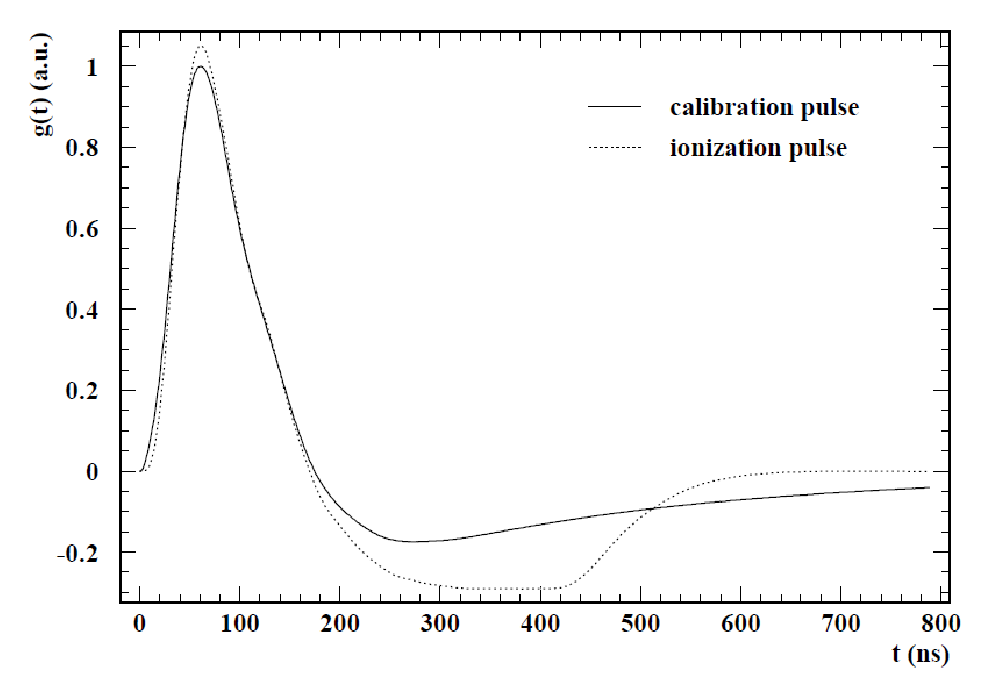
\includegraphics[width=0.6\linewidth,angle=0]{Detector/calibration_pulse_shape}
\end{center}
\caption[Calibration and ionisation pulses in the EMB.]{Calibration and ionisation pulse shapes for an EMB channel, after shaping. Prior to shaping, the peak current of the two pulses were equal~\cite{cell_equal}.}
\label{fig_calibpulsehape}
\end{figure}

Delay runs allow the pulse shapes to be measured. In delay runs, the calibration pulse is delayed (with respect to the TTC clock) by multiples of 1 ns. This effectively allows the shaped calibration pulse to be sampled at 1 ns intervals, which gives an accurate measurement of the shape of the calibration pulse. This information may then be used to infer the final shape of pulses originating from ionisation\cite{cell_equal}, which may then be used (together with the noise autocorrelation information obtained from pedestal runs) to derive the OFCs used for data taking at \atlas. The factor $M_\mathrm{phys}/M_\mathrm{calib}$ describes the ratio of the shaped ionisation pulse amplitude to that of the shaped calibration pulse amplitude, for cases in which both pulses have the same peak current prior to shaping. This factor corrects for the effect of pulse shaping, and thus allows the calibration factors (which are derived from calibration pulses) to be used for the calibration of ionisation pulses. 

For the FCal\label{FCal_ecal_page}, the calibration is based on testbeam studies rather than derived using calibration pulses. The factor $F_{\mu\mathrm{A}\rightarrow\mathrm{MeV}}$ may be calculated for each module from the geometry of the FCal electrodes and the other properties of the detector. The ADC2MeV value obtained from testbeam can then be used to derive a value of $F_{\mathrm{DAC} \rightarrow \mu\mathrm{A}}$ that is appropriate for the electronics used in \atlas. As the calibration is not derived from calibration pulses, the factor $\frac{1}{M_\mathrm{phys}/M_\mathrm{calib}}$ is not needed. Pedestal runs are used to measure noise in the electronics, but pulse shapes from testbeam data are used in the calculation of the OFCs (delay runs are not taken for the FCal). Ramp runs are still used to obtain $R$, and can thus be used to correct for any variations in the electronic gains.

%fuck you

%
% however the ramp runs are used to calculate the value of $R$.
%
% only pedestal runs and ramp runs are taken during electronic calibration.
%The OFCs are computed using the noise measured during pedestal runs with pulse shapes obtained from testbeam data. The factors 





  

%The factor 1/M/M corrects for this effect, thus allowing values of F derived from calibration pulses to be used to calibrate pulses caused by ionisation in the calorimeter. \red{mention that this requires knowledge of the ionisation pulse shape. But calibration data allows certain electrical properties of the readout chain to be measured, and analysis of the readout electronics then allows the shape of an ionisation pulse to be inferred from the (measured) calibration pulse shape.Cite cell response equal}
%
%So, for equation \ref{}, the factors R\times F_dac->muA equate to an ADC->muA factor appropriate for calibration pulses, while the M/M factor corrects this such that it may be used for ionisation pulses. Finally, the FmuA->GeV converts the electrode current into the ionisation energy deposited in the active region of the calorimeter, and scales this value by the sampling fraction of the calorimeter. 
%
%cite cell response equal, electronic_calibration, LAr_electronics
%
%%liquid argon electronics, electrode current is triangular peak so signal current is just charge deposited in active region via ionisation divided by the maximum electron drift time. the factor F may thus be obtained from geant4 simulations of the calorimeter, comparing the amount of energy deposited in the active regions via ionisation to the total amount of energy deposited in the calorimeter.
%%
%This factor must be determined from either 
%
%need an ADC2GEV factor.
%find this from calibration runs. 
%
%

%\clearpage


%
%
%TGCs
%
%RPCs
%
%
%
%
%toroidal magnets, barrel and two end-caps
%
%four systems Monitored Drift Tubes, Cathode Strip Chambers, Resistive Plate Chambers, Thin Gap Chambers
%
%TGC's and RPC's used for triggering, MDT's and CSC's used for measurement




\subsection{Trigger and Data Acquisition}
\label{sec_triggers}
%Do electron triggers work the same way as jet triggers?
%
%talk about jet triggers, or just triggers in general. Don't go into specifics about electrons and muons.
%
%% forward jet triggers - split in phi into two ``pseudo'' jet elements, then algorithm is run. Equivalent to requiring trigger tower to pass the threshold.
%
%at design, bunches cross every 25ns. need trigger to decide which events to write out.
%Three levels, L1, L2, and EF. L2 and EF make up the HLT. L1 is hardware, L2 is hardware/software.
%
%L1 has to make a decision within XX. 
%
%definitely need some data quality


%interactions occur at a rate of 40 MHZ. too often to record every event
%
%trigger used to determine which events are interesting and should thus be written out
%
%maximum accept rate at L1 is 75 kHz

\cmt{simple/complex deadtime?}

Collisions between proton bunches occur at \atlas at a design rate of 40 MHz, however, the maximum rate at which events can be recorded is limited by computing resources and is presently $\sim 400$ Hz\cmt{\footnote{The trigger system was originally designed to record events at $\sim 200$Hz, but is currently functioning at a much higher rate}}. The trigger system is designed to ensure that as many interesting events are recorded as possible, while rejecting less interesting events that occur at high rates, as shown in Figure~\ref{SMxsec}.\cmt{\red{could put the cross section plot of SM processes in here}} The \atlas trigger system consists of three consecutive levels: level one (L1), level 2 (L2), and the Event Filter (EF). The L1 trigger selects candidate events at a maximum rate of 75 kHz. Most of these events are subsequently rejected at L2, reducing the acceptance rate to 3.5 kHz. The final level of event rejection is done by the EF, which accepts events at the desired rate of $\sim 400$ Hz. 

%The L2 and EF together form the High Level Trigger, however until recently only the L1 trigger has been used for selecting forward jet events. 

The L1 trigger utilises custom-built hardware that is located off the detector, and needs to decide whether to accept or reject the event within 2.5 $\mu$s of the corresponding bunch crossing. While this decision is being made, information from detector channels is stored in pipeline memories, which are located on or near the detector.  The level 1 trigger consists of three of three parts, L1 Calo, L1 Muon, and the Central Trigger Processor (CTP). The L1 Calo trigger is used to select electrons, jets, taus, and other high \pt~ objects (excluding muons), while the L1 muon trigger processes signals from the RPCs and TGCs of the Muon Spectrometer. 

The CTP decides whether an event is accepted or rejected at L1. Trigger conditions are specified in a ``menu",  each item of which is some combination of trigger items from L1 Calo and/or L1 Muon. The CTP also handles the ``prescales'' on these menu items, which are used to control the bandwidth allowed for each item and keep the L1 acceptance rate at the desired level. For a menu item with a prescale of 50, one event will be accepted at L1 for every fifty events that satisfy the trigger conditions associated with that menu item. Menu items associated with a rare or particularly interesting event topology may be given a prescale of one, in which case the event is accepted every time the trigger conditions are met. Frequently occurring or less interesting topologies (such as those containing low-\pt~ jets) are given higher prescales.  
%
%
%
%%
%%Note that while the maximum rate at which events can be accepted at L1 is 75 kHz, during 2010 running this rate did not exceed 30kHz~\cite{trigger_2010}.
%%
%%things to add
%%detector data stored in buffers while waiting for L1A signal
%%L1A max latency of 2.5 us. nominally 2.1us. ``Large Fraction of this'' is in transmission time for signals to and from detector electronics.
%%L1 calo - custom electronics located off detector - decision made in less than 1us
%
%trigger towers - analogue sums 


The CTP also receives input from specialised detectors, such as ALFA (Absolute Luminosity For ATLAS), LUCID (Luminosity measurement using a Cherenkov Integrating Detector), the Beam Conditions Monitor (BCM) and the Minimum Bias Trigger Scintillators (MBTS). LUCID~\cite{LUCID} and ALFA~\cite{ALFA} are luminosity detectors located 17m and 240m from the \atlas interaction point, respectively, and were used to measure the luminosity delivered to \atlas during 2010. The BCM~\cite{BCM} is designed to monitor the condition of the beams and identify situations in which beams may be harmful to \atlas detectors (triggering a beam abort). It also provides a real time measurement of the luminosity at \atlas. The MBTS is used to select ``minimum bias'' events: the thresholds required to accept these events are very low, and so collision events are selected with minimal bias. These events are typically soft inelastic scatterings. The MBTS consists of tiles of scintillating polystyrene that are 2cm thick. There are 16 of these tiles mounted on the outer wall of each end-cap cryostat (on the side closest to the interaction point), covering the pseudorapidity range $2.09 < |\eta| < 3.84$. Early studies of the MBTS showed it to be very efficient, with an efficiency of over 99\% for selecting events in which there were at least 3 tracks with $\pt > 100$MeV~\cite{Tompkins_minbias}. Because of its high efficiency and low bias, the MBTS trigger was used as a reference when determining the efficiency of the jet triggers used in the inclusive jet and dijet cross section measurements, as discussed in section~\ref{incjet_triggers}. The distribution of charged particles obtained from minimum bias events recorded at \atlas is plotted in Figure~\ref{minbiasplot}~\cite{atlas_minbias}. Note that the distribution is roughly uniform in $\eta$. Due to the nonlinear relationship between $\eta$ and the polar angle, $\theta$, a fixed interval $\Delta \eta$ corresponds to a smaller angular interval at high $|\eta|$ than at low $|\eta|$. For example, one side of the EM Barrel has a length of 3.2 metres and covers the region $0<\eta<1.475$, while the FCal has an outer radius of $\sim450$mm and covers the region $3.2<\eta<4.9$: the FCal covers a larger pseudorapidity interval in a much smaller area. As the distribution of particles produced in minimum bias events varies slowly in $\eta$, detectors covering higher values of $\eta$ will be subject to a higher flux of particles than detectors located at low $\eta$. The effects of pile up are thus more significant for the FCal and end-cap calorimeters than for the barrel calorimeters.

\begin{figure}[tb]
\begin{center}
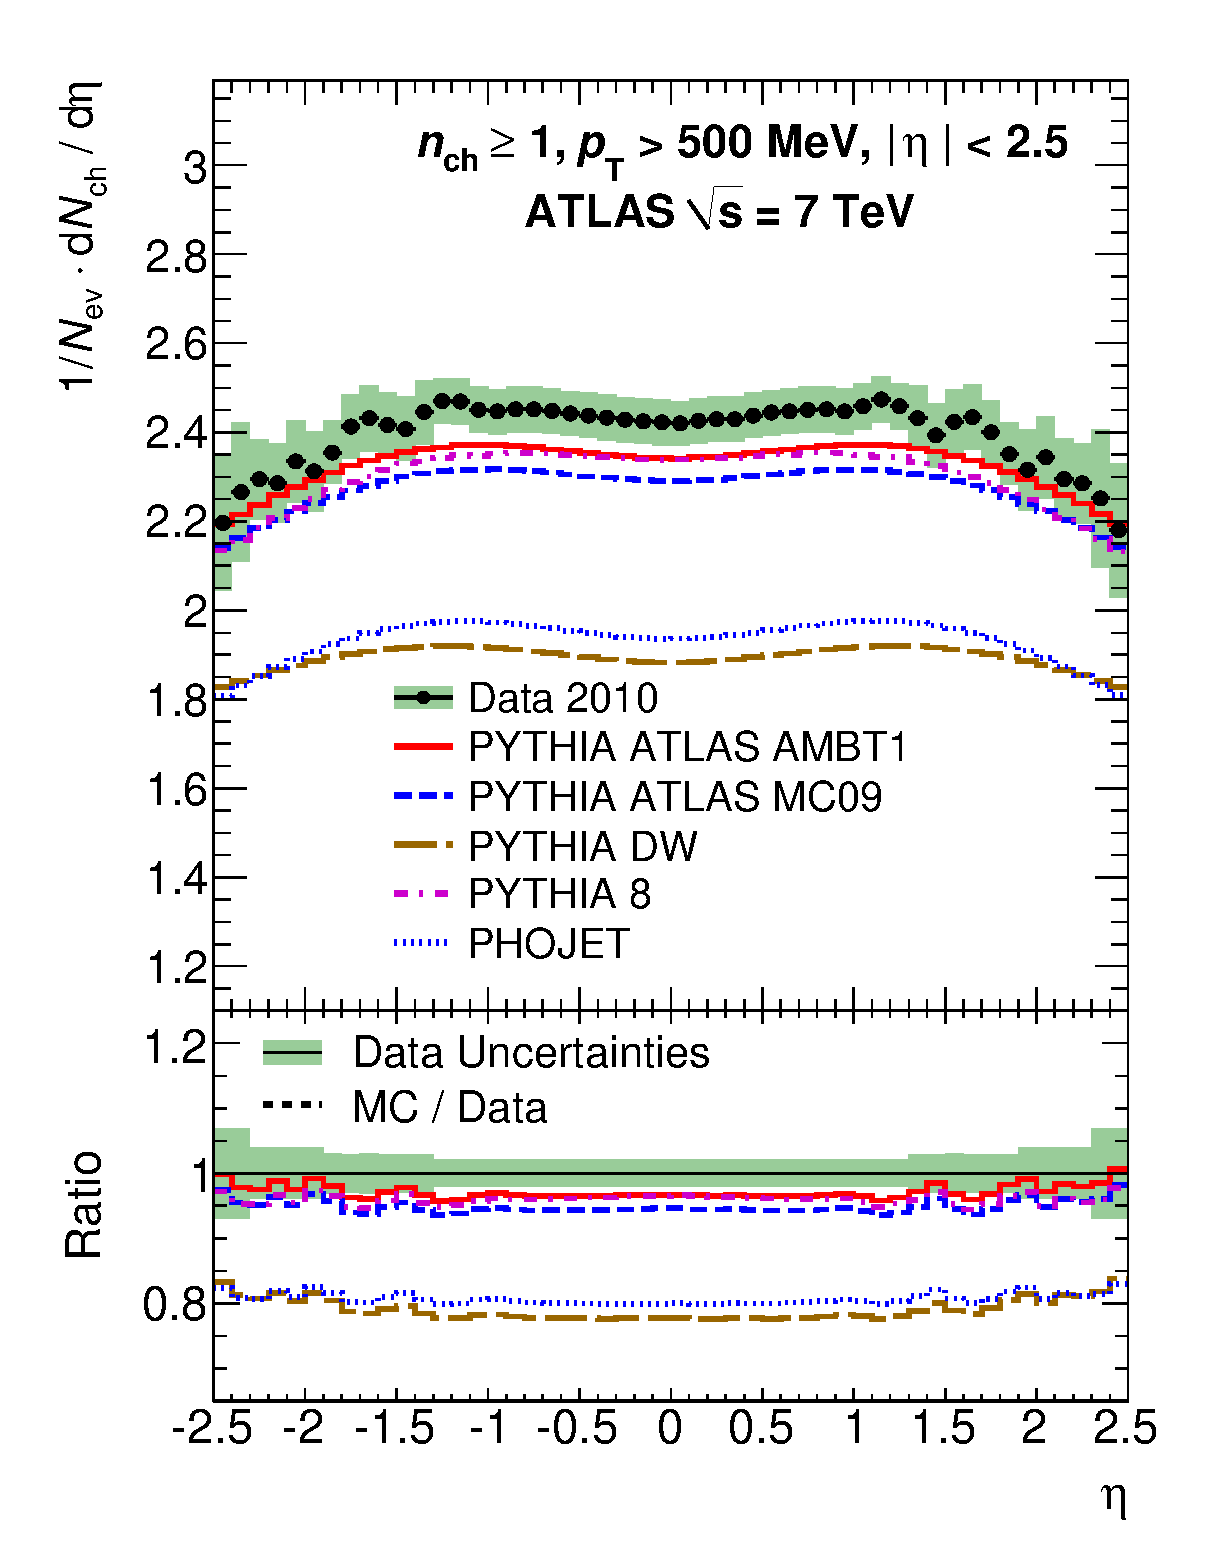
\includegraphics[width=0.6\linewidth,angle=0]{atlas_7tev_minbias.eps}
\end{center}
\caption[Distribution of charged particles in minimum-bias events.]{Distribution of charged particles produced in minimum bias events\cite{atlas_minbias}. The plot shows data measured at ATLAS, as well as predictions obtained from Monte Carlo simulations using a variety of tunes. Note that the plot only covers the region $-2.5 < \eta < 2.5$, as Inner Detector coverage is limited to this interval.}
\label{minbiasplot}
\end{figure}

The time available for the L1 decision is too short for L1 Calo to consider the information from individual calorimeter cells. Cell information is stored in the detector electronics, and only read out when an L1 accept signal is received from the CTP. Of the 2.5 $\mu$s available at L1, the decision is usually made within 2.1$\mu$s. However, a large fraction of this time is taken up by the transit time for signals to propagate between the trigger hardware and the detector, while L1 Calo processes events in less than 1 $\mu$s. Instead of relying on cell information, calorimeter signals are instead processed into ``trigger towers'', which are then sent as input to L1 Calo. Trigger towers are formed from analog sums of readout channel signals, as discussed in Section~\ref{sec_FEB}. In the Tile calorimeter, a trigger tower is formed by summing the signals from five channels. In the LAr calorimeters, the first two stages of summation are carried out on the FEBs, while the remaining addition is carried out on dedicated Tower Builder Boards (for the EMB and EMEC) or Tower Driver Boards (for the HEC and FCal)\cite{ATLAS_front_end_electronics}. In the barrel and end-cap regions $(|\eta| < 3.2)$, the trigger towers have a granularity 0.1$\times$0.1 in $\eta$ and $\phi$, whereas in the FCal the trigger towers have a granularity of approximately 0.4 $\times$ 0.4.

\subsubsection{Jet Triggers}

The level 1 central jet trigger combines 2$\times$2 blocks of trigger towers to form ``jet elements", which then have a granularity of  0.2$\times$0.2 in $\eta - \phi$ space. A sliding window algorithm\cite{ATLAS_L1Calo} is then used to identify jets. The window consists of a 4$\times$4 grid of jet elements, and a jet is identified if the total transverse energy within the window exceeds a given threshold. For example, the ``L1\_J10'' algorithm requires the transverse energy (at the EM scale) in the window to exceed 10 GeV. Additionally, the $2 \times 2$ cluster of jet elements in the centre of the window is required to be a local maximum; that is, the central cluster must have a transverse energy greater than that of any other $2\times2$ block of jet elements within the window.\cmt{ higher than any other cluster on two sides, equal or greater on other two}. If these criteria are met, then the event is accepted by the jet algorithm. The $0.4\times0.4$ area of $\eta-\phi$ at the centre of the window is then identified as a ``Region of Interest'' (ROI), and is passed on to any relevant L2 trigger algorithms. 

The forward jet trigger is used to identify jets in the region $|\eta| > 3.2$, and operates independently of the central jet trigger. While the central jet trigger uses information from the EM Barrel, Tile, EMEC and HEC calorimeters, only the forward jet trigger uses information from the FCal. Trigger towers in the FCal have a granularity of $\sim$0.4 $\times$ 0.4 in $\eta-\phi$, which is coarser than in other calorimeters. A jet element is then formed by summing all FCal trigger towers in $\eta$, such that the jet element has dimensions 1.6 $\times$ 0.4 in $\eta$ and $\phi$, respectively\cite{ATLAS_L1Calo}. Jets are then identified using the same sliding window algorithm that is used by the central jet trigger\cite{JEM_spec}.


At L2, the trigger decision needs to be made within 40ms. This interval is sufficient for cell-based methods to be used, although only cells within the region of interest (typically about 2\% of the detector) are read out. A cone-based algorithm is used for jet identification: a cone of fixed radius $\Delta R = \sqrt{\Delta \eta^2 + \Delta \phi^2}$ is positioned at the centre of the RoI. Energy weighted values of $\eta$ and $\phi$ are obtained by summing cells within the cone, and the centre of the cone is then moved to these coordinates. This process is carried out a predetermined number of times.

At the EF level, 4.0s of processing time is available, and so algorithms similar to those used for offline reconstruction (described in section~\ref{incjets_jetfinding}) may be used at the trigger level. Note that EF algorithms for jet triggers were not online while the data used in this thesis were being recorded, and so the trigger studies presented in section~\ref{incjet_triggers} focus on jet triggers at L1 and L2.



%At level 2

%The level 1 trigger is built on custom hardware utilising FPGAs, and needs to decide whether to accept or reject the event within 2.5 $\mu$s of the corresponding bunch crossing. 
%calo trigger

%L1 uses trigger towers. if accepted, identifies a RoI and passes this to L2. L2 looks at cells in the RoI, and has access to muon chambers and inner detector information. 
%
%Jet triggers blah blah. central Jet trigger covers uses up to eta < 3.2, while dedicated forward jet trigger uses information solely from the FCal. handy to use for triggering on events with forward jets, such VBF, where forward jets may be used to tag VBF event. 
%
%jet algorithms work like this at L1. Central trigger towers have this granularity.
%
%forward jet towers have this granularity, and so the L1 trigger does this.
%
%at L2 a cone algorithm is used.


%The level one trigger system is comprised of custom built hardware, and must decide whether to accept or reject an event within 2.5 $\mu s$ of the bunch crossing. This time interval is too short to look at detailed calorimeter cell information, and so the calorimeters are divided into trigger towers. In the central region, these have a granularity of 0.1$\times$0.1 in $\eta$ and $\phi$. The L1 jet trigger forms jet elements by summing 2$\times$2 blocks of trigger towers, thus giving an $\eta-\phi$ granularity of $0.2\times0.2$\cite{ATLASTrigger}. A sliding window algorithm is then run on the jet elements, and a jet is found if the transverse energy of a 2x2 cluster of elements from within the window passes a certain threshold. If so, the area is flagged as a region of interest and passed to the level two trigger. 
%
%Trigger towers in the FCal are more coarsely grained than in the central region, having a width of $0.4\times 0.4$ in $\eta-\phi$. Here the jet elements are formed by summing all towers in a phi slice, giving no granularity in $\eta$. 

